\documentclass[
BCOR0.7cm,							% Bindekorrektur, bspw. 1 cm
]
{scrbook}

\newif\ifpdf
\ifx\pdfoutput\undefined
	\pdffalse              	%normales LaTeX wird ausgef�hrt
\else
	\pdfoutput=1           
	\pdftrue               	%pdfLaTeX wird ausgef�hrt
\fi

\ifpdf
	%\usepackage{ae}        % Benutzen Sie nur
	%\usepackage{zefonts}  	% eines dieser Pakete
\else
	%%Normales LaTeX - keine speziellen Fontpackages notwendig
\fi

\ifpdf %%Einbindung von Grafiken mittels \includegraphics{datei}
	\usepackage[pdftex]{graphicx} %%Grafiken in pdfLaTeX
\else
	\usepackage[dvips]{graphicx} %%Grafiken und normales LaTeX
\fi

\ifpdf
	\pdfinfo
	{
    /Author (Rudolf Hangl)                                
    /Title (FAS-Online)     
    /Subject (Benutzerhandbuch FAS-Online)                                    
    /Keywords (FAS FH-Complete Technikum-Wien)
	}
\else			
\fi

\usepackage{listings} \lstset{numbers=left, numberstyle=\tiny, numbersep=5pt}
\lstset{language=tex} 


\usepackage[pdftex,colorlinks=true,urlcolor=blue,linkcolor=blue]{hyperref}
\usepackage[ngerman]{babel}		
\usepackage[T1]{fontenc}
\usepackage[latin9]{inputenc}
\usepackage{makeidx}
\usepackage{float}
\usepackage[small,bf]{caption}
\usepackage{fancyhdr}
\usepackage{amssymb,amsmath}
\makeindex

\graphicspath{{../../images/}}

\setlength{\tolerance}{2000}
\setlength{\parindent}{0pt}
\setlength{\parskip}{1ex plus 0.5ex minus 0.2ex}
\addtolength{\textheight}{2cm}
\addtolength{\headheight}{2pt}
\setlength{\captionmargin}{20pt}
\floatstyle{plain}
\floatname{example}{Example}

\newfloat{example}{hbtp}{loe}[chapter]
\floatplacement{figure}{hbtp}
\floatplacement{table}{htbp}

\newcommand{\dollar}{\char36}

\newenvironment{info}[1]{
    \hspace{-10mm}
    \fbox{
        \begin{minipage}{1cm}
        
\includegraphics[width=1cm]{icon_info}
        \end{minipage}
        \begin{minipage}{14.5cm}
        #1
        \end{minipage}
    }
}

\newenvironment{achtung}[1]{
    \hspace{-10mm}
    \fbox{
        \begin{minipage}{1cm}
        
\includegraphics[width=1cm]{icon_achtung}
        \end{minipage}
        \begin{minipage}{14.5cm}
        #1
        \end{minipage}
    }
}

\newenvironment{halt}[1]{
    \hspace{-10mm}
    \fbox{
        \begin{minipage}{1cm}
        
\includegraphics[width=1cm]{icon_halt}
        \end{minipage}
        \begin{minipage}{14.5cm}
        #1
        \end{minipage}
    }
}

\newenvironment{idee}[1]{
    \hspace{-10mm}
    \fbox{
        \begin{minipage}{1cm}
        
\includegraphics[width=1cm]{icon_idee}
        \end{minipage}
        \begin{minipage}{14.5cm}
        #1
        \end{minipage}
    }
}


\setlength{\unitlength}{1mm}

\newenvironment{markier}[5]{
    
    \thicklines \put(#2,#3){\vector(#4,#5){5}} \thinlines
    \put(#2,#3){\circle*{5}}
    \put(#2,#3){\textcolor{black}{\circle{5}}\makebox(-10,0){\textcolor{white}{#1}}}


}


\hyphenation{gleich-zeitig para-meter}


\begin{document}

\ifpdf
	\DeclareGraphicsExtensions{.pdf,.jpg,.png}
\else
	\DeclareGraphicsExtensions{.eps}
\fi

\pagestyle{fancyplain}
% Titelseite einbinden
%
% Titelseite, Abstrakt, Danksagung und Inhaltsverzeichnis
%
%% eigene Titelseitengestaltung %%%%%%%%%%%%%%%%%%%%%%%%%%%%%%%%%%%%%%%    

\begin{titlepage}
\begin{center}
\vspace*{40mm} \huge Benutzerhandbuch\\
\vspace*{10mm}
\vfill 
\includegraphics[width=130mm]{logo_fas}
	
\large \vfill \textsc{Technikum Wien}\\

Wien, \today
\end{center}
\end{titlepage}


\tableofcontents			% Inhaltsverzeichnis
\frontmatter					% Vorspann (z.B. r�mische Seitenzahlen)
\chapter{Einleitung}
\mainmatter						% Hauptteil

%% Kapitel Anfang %%%%%%%%%%%%%%%%%%%%%%%%%%%%%%%%%%%%%%%%%%%%%%%%%

\chapter{Grundlagen}
\achtung{\textbf{Wichtig} FAS bitte nur \textbf{einmal} �ffnen!\\
	Gleichzeitiges Arbeiten mit mehreren Instanzen von FASonline kann zu Aktualisierungsproblemen bei Semesterwechseln f�hren.}\\

\section{Aufbau der Arbeitsoberfl�che}
\begin{figure}
	\begin{center}
    \begin{picture}(128,89)
			\put(0,0){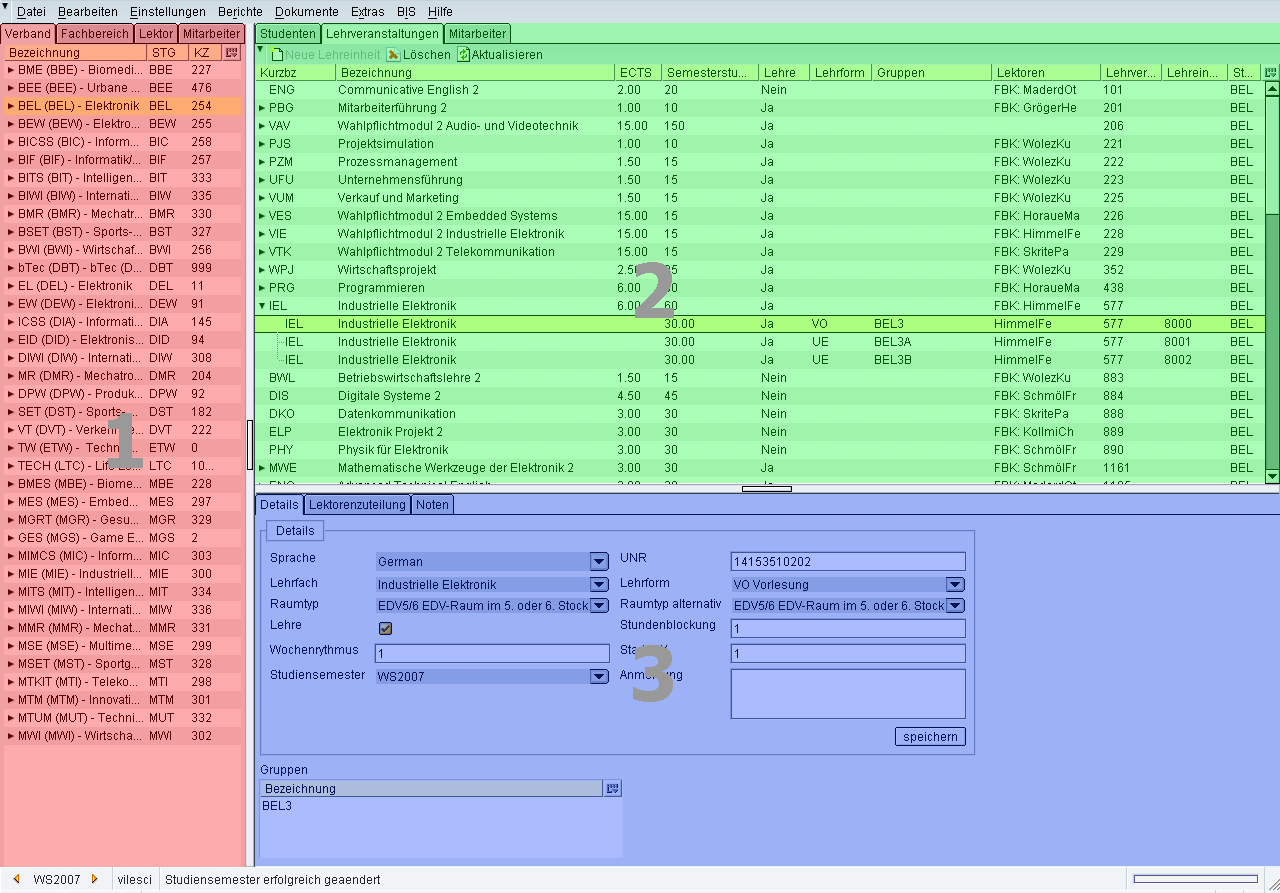
\includegraphics[height=89mm, width=128mm]{FAS_Grundlagen1.png}}
			\markier{4}{6}{8}{0}{-1}
			\markier{5}{20}{8}{-1}{-1}
		\end{picture}
    \caption{Aufbau der Oberfl�che}
		\label{Grundlagen1}
  \end{center}
\end{figure}
\subsection{Listenfeld 1}
\begin{itemize}
	\item Verband: In dieser Karteikarte werden nur die Studieng�nge angezeigt, f�r die der Anwender Zugriffsrechte besitzt. Wenn es zu einer Zeile Untergruppierungen gibt, wird links neben dem Namen ein Symbol angezeigt. Abbildung \ref{Grundlagen2} zeigt den strukturellen Aufbau eines Studiengangs. 
\begin{figure}
	\centering
	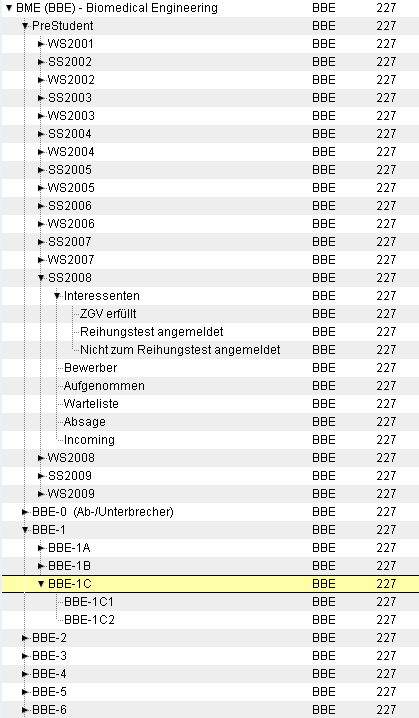
\includegraphics[width=0.55\textwidth]{FAS_Grundlagen2.png}
	\caption{Anzeige Stundiengang}
	\label{Grundlagen2}
\end{figure}
		\begin{itemize}
			\item Prestudent: 
			Als Prestudent werden alle Personen bezeichnet die noch keine Studenten sind (\textsl{pre}(lat.) - \textsl{vor}). Die Aufteilung der Prestudenten erfolgt in Semester und da dann noch in verschiedene Interessenten sowie Bewerber, Aufgenommene, Personen auf der Warteliste und Personen die abgesagt haben bzw. denen abgesagt wurde.
			Weiters finden sich hier die Incoming \underline{aller} Studieng�nge dieses Semesters.
			\item Semester: Es werden immer alle Semester mit Lehrverb�nden und Gruppen angezeigt, auch die in diesem Semester nicht aktiven. 
		\end{itemize}
	\item Institut: Zur Anzeige der Institutsliste mu� nach �ffnen der Karteikarte die Taste 
\includegraphics{icon_aktualisieren} angeklickt werden. Die Liste z�hlt die Institute und die zugeordneten Lektoren auf. Markiert man einen Lektor erscheinen im Listenfeld 2 alle Lehrveranstaltungen dieses Fachbereichs, in denen dieser Lektor unterrichtet. 
	\item Lektor: Alle Lektoren auch zugeteilt zu Studieng�ngen.
	\item Mitarbeiter: Mehrere Listenansichten dem Mitarbeiter gefiltert nach den in Abbildung \ref{Grundlagen3} gezeigten Kriterien. Die Anzeige der Lektoren erfolgt in Listenfeld 2.
	\begin{figure}
		\centering
		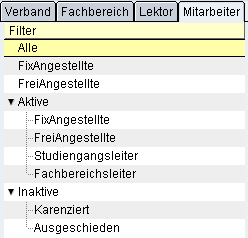
\includegraphics[width=0.55\textwidth]{FAS_Grundlagen3.png}
		\caption{Anzeige Mitarbeiter}
		\label{Grundlagen3}
	\end{figure} 
\end{itemize}
\subsection{Listenfeld 2}
\begin{itemize}
	\item Studenten: Liste von Studenten, gefiltert nach der Auswahl in Listenfeld 1 oder einer Suche.
	\item Lehrveranstaltungen: Liste von Lehrveranstaltungen mit zugeordneten Lehreinheiten, gefiltert nach Auswahl in Listenfeld 1.
	\item Mitarbeiter: Anzeige von Mitarbeiter, gefiltert nach der Auswahl von Listenfeld 1.
\end{itemize}
\subsection{Datenbereich}
Die Anzeige in diesem Teil ist von der Auswahl im Listenfeld 2 abh�ngig und zeigt Detaildaten an bzw. k�nnen diese hier eingegeben und ge�ndert werden.\\
Bei Auswahl in Listenfeld 2 zeigt der Datenbereich folgende Karteikarten:
\begin{itemize}
	\item Studenten: 	
	\begin{itemize}
		\item Details - Kapitel \ref{details}
		\item Kontakt - Kapitel \ref{kontakte}
		\item PreStudent - Kapitel \ref {prestudent}
		\item Dokumente - Kapitel \ref{dokumente}
		\item Konto - Kapitel \ref{studentenkonto}
		\item Betriebsmittel - Kapitel \ref{betriebsmittel}
		\item In/Out - Kapitel \ref{Incoming} und \ref{Outgoing}
		\item Noten - Kapitel \ref{noten}
		\item Zeugnis - Kapitel \ref{zeugnis}
		\item Pr�fung - Kapitel \ref{pruefungen}
		\item AbschlussPr�fung - Kapitel \ref{abschlusspruefungen}
		\item Projektarbeit - Kapitel \ref{projektarbeit}
		\item Gruppen - Kapitel \ref{gruppen}
		\item Funktionen - Kapitel \ref{funktionen}
	\end{itemize}
	\item Lehrveranstaltungen - Kapitel \ref{lehrveranstaltung}: 
	\begin{itemize}
		\item Details 
		\item Lektorenzuteilung 
		\item Noten
	\end{itemize}
	\item Mitarbeiter - Kapitel \ref{mitarbeiter}:
	\begin{itemize}
		\item Stammdaten 
		\item Kontaktdaten
		\item BIS-Daten
		\item Betriebsmittel 
		\item Funktionen
	\end{itemize}
\end{itemize}
\subsection{Statusleiste}
\begin{itemize}
	\item 4 Studiensemester: Die Anzeige besteht aus drei Tasten. Die mittlere Taste zeigt das aktuell eingestellte Semester, mit einem Klick auf die Taste wird die Anzeige aktualisiert. Diese Funktion ist dann wichtig, wenn FASonline mehrmals ge�ffnet ist oder gleichzeitig Tempus verwendet wird, da das Semester in bei einer �nderung in einem Fenster in den anderen Fenstern nicht automatisch sondern nur mit Tastendruck aktualisiert wird.\\
Mit beiden Pfeiltasten kann ins jeweils vorige (links) und n�chste Semester (rechts) geschalten werden.
	\item 5 Datenbankanzeige: Zeigt den Namen der aktuell verwendeten Datenbank an.
\end{itemize}
\chapter{Studenten}
\label{studenten}
\section{Stati}
Ein Student erh�lt im Zuge seiner Studentenkarriere verschiedene Stati zugewiesen.
\begin{itemize}
	\item Abbrecher: Person, die das Studium ohne Abschlu� beendet hat.\\Student mu� UID besitzen. Das \textit{Aktiv}-H�kchen mu� entfernt werden!
	\item Abgewiesener: Person, die nicht zum Studium zugelassen wurde.
	\item Absolvent: Person, die das Studium mit Abschlu� beendet hat.\\Student mu� UID besitzen. Das \textit{Aktiv}-H�kchen mu� entfernt werden!
\\
\textbf{Achtung}, werden Absolventen auf inaktiv gesetzt, werden sie aus den E-Mail-Verteilern entfernt! 
Die E-Mail-Adressen selbst sind davon nicht betroffen.
 
	\item Aufgenommener: Person, die zum Studium zugelassen wird.\\Ein Status Bewerber mu� vorhanden sein.
	\item Bewerber: Person, die den Reihungstest bestanden hat.\\Datum f�r \textit{Anmeldung zum Reihungstest} mu� eingeben sein, \textit{Zum Reihungstest angetreten} mu� angekreuzt sein.
	\item Diplomand: Person, die das Studium abgeschlossen hat und vor der Abschlu�pr�fung steht. Jeder Student, der die Berechtigung zum Antritt zur Abschlu�pr�fung erreicht, wechselt in den Status Diplomand.\\
	Die BIS-Meldung sieht vor, da� Studenten, die erst sp�ter zur Pr�fung antreten, mit der Semesteranzahl 50 (entspricht 2-3 Eintragungen eines Diplomandenstatus) f�r die Absolvierung der Abschlu�pr�fung innerhalb eines Jahres oder Semesteranzahl 60 (entspricht 4 oder mehr Eintragungen eines Diplomandenstatus) f�r einen l�ngeren Zeitraum gemeldet werden m�ssen.
	\item Incoming: Studenten anderere FHs, die hier Auslandssemester absolvieren.
	\item Interessent: Person, die Interesse am Studiengang bekundet hat.\\Nachname, Vorname, Geburtsdatum, Geschlecht m�ssen eingegeben sein. Status wird beim Anlegen vergeben.
	\item Student: Person, die im Studiengang inskribiert ist.\\\textit{ZGV} mu� ausgew�hlt sein, bei Masterstudieng�ngen auch \textit{ZGV Master} und ein Status Bewerber und Absolvent mu� vorhanden sein.
	\item Unterbrecher: Karenzierter Student.\\Student mu� UID besitzen.
	\item Wartender: Bewerber auf einer Warteliste, der nachr�cken kann, wenn ein inskribierter Student bis kurze Zeit nach Beginn des Startsemesters ausf�llt.\\Ein Status Bewerber mu� vorhanden sein.
\end{itemize}
Abbildung \ref{Statusverlauf} zeigt die Abfolge der Prestudentrollen (Stati).
\begin{figure}
	\centering
	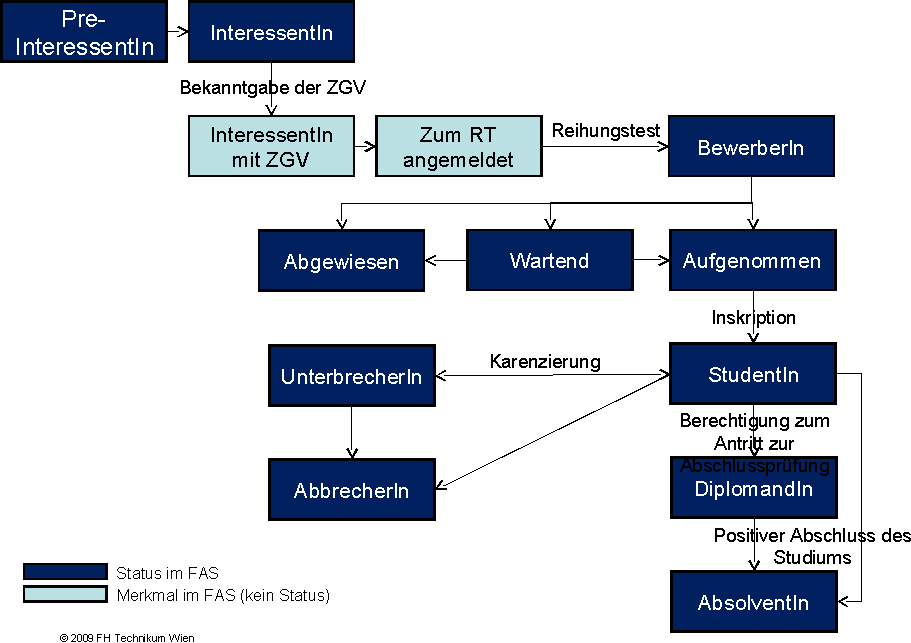
\includegraphics[width=1\textwidth]{FAS_Statusverlauf.png}
	\caption{Statusfolge}
	\label{Statusverlauf}
\end{figure}
\section{Anlegen eines neuen Interessenten}
\label{Anlegen eines neuen Interessenten}
Abbildung \ref{Interessent1} zeigt das Formular zum Anlegen eines Interessenten. Es gibt nun zwei Arten, dieses Formular auszuf�llen:
\begin{enumerate}
	\item manuell: Das Formular wird mit der Taste 
\includegraphics[width=10mm]{../../images/icon_neu.png} aufgerufen und die Eingabefelder m�ssen dann mit den Interessentendaten bef�llt werden.
	\item E-Mail: Es besteht auch die M�glichkeit �ber die offizielle Technikum Wien - Homepage www.technikum-wien.at Kontakt mit den Studieng�ngen aufzunehmen. Es kann dort ein Formular ausgef�llt und per E-Mail (siehe Abbildung \ref{Interessent2} an den betreffenden Studiengang geschickt werden. Auf diesem E-Mail befindet sich ein Link \textsl{Bewerbung ins System �bertragen}, mit dem diese Daten in das Formular eingetragen weden. 
\end{enumerate}
Nachdem die Eingabefelder bef�llt wurden, sollte �berpr�ft werden, ob der Interessent bereits in der Datenbank vorhanden ist. Durch Dr�cken des Knopfs \textsl{Vorschlag laden} werden die Eingabedaten verglichen und m�gliche Treffer rechts neben der Eingabemaske ausgegeben. Befindet sich der Interessent bereits in der Datenbank, kann einer der Vorschl�ge geladen oder ein neuer Interessent angelegt werden. Die Auswahl wird mittels Radio-Buttons angegeben.
\begin{figure}
	\centering
	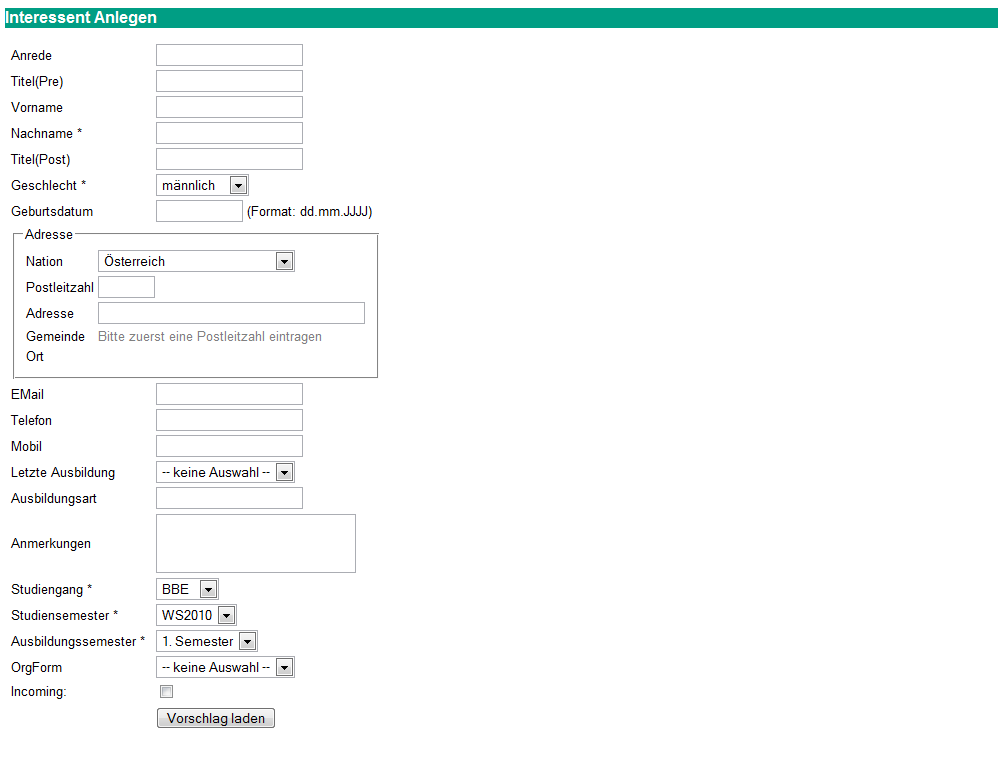
\includegraphics[width=0.75\textwidth]{FAS_Interessent1.png}
	\caption{Interessenten anlegen}
	\label{Interessent1}
\end{figure}
\begin{figure}
	\centering
	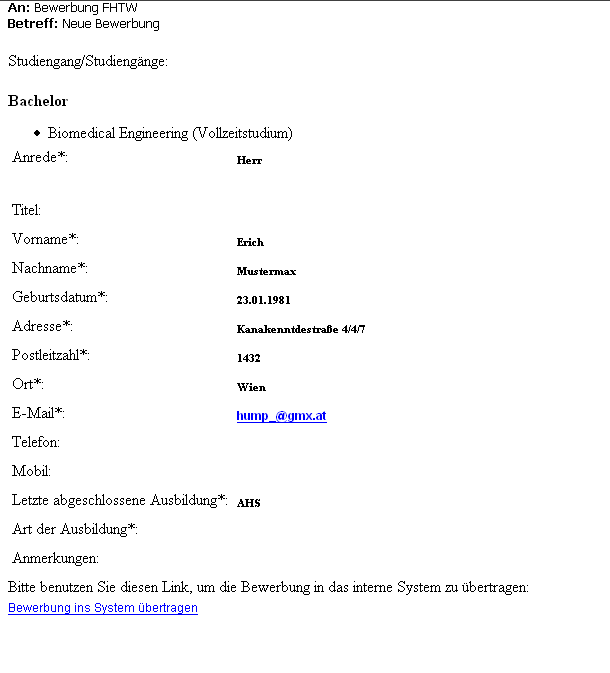
\includegraphics[width=0.75\textwidth]{FAS_Interessent2.png}
	\caption{Interessentenmail}
	\label{Interessent2}
\end{figure}
\subsection{Ablauf Interessenten anlegen}
\idee{\textbf{Hinweis:} Ein Student kann kein zweites Mal in einem Studiengang angelegt werden!}\\

\begin{enumerate}
	\item Karteikarte \textit{Verband} im Listenfeld 1 ausw�hlen.
	\item In der Karteikarte \textit{Student} des Listenfeld 2 die Taste 
\includegraphics{icon_neu.png} anklicken.
	\item Es �ffnet sich die Eingabemaske.
	\item Eingabemaske bef�llen:
	\begin{itemize}
		\item Mit * markierte Felder m�ssen bef�llt bzw. ausgew�hlt werden.
		\item Da es sich hier um einen Interessenten und keinen Incoming handelt, darf die Checkbox \textit{Incoming} nicht angekreuzt werden!\\
\textbf{Achtung}, beim Anlegen des Incoming werden auch dessen Personenkennzeichen und UID erzeugt. Eine nachtr�gliche �nderung ist mit einigem Aufwand verbunden.
 
	\end{itemize}
	\item Beim Klicken auf 'Vorschlag laden' wird gepr�ft, ob diese Person bereits im System vorhanden ist. Wenn dies der Fall ist, muss in der rechten Spalte die Person markiert werden. Andernfalls w�hlen Sie den Eintrag neue Person aus. Wenn die vorhandene Person verwendet wird, werden die Stammdaten (SVNR, Geburtsdatum, Kontaktdaten, etc) von der bereits vorhandenen Person �bernommen.\\
	\textbf{Achtung}, wenn Sie hier eine neue Person anlegen, obwohl die neue Person bereits im System vorhanden ist, kann es in weiterer Folge zu Problemen beim Eintragen der Sozialversicherungsnummer oder bei Zutrittskarten kommen.
	\item Durch Dr�cken der Taste \textit{Speichern} werden die Daten in die Datenbank �bertragen.
\end{enumerate}
\subsection{PreInteressenten}
Personen die sich f�r ein Studium Interessieren, sich aber noch nicht f�r einen Studiengang entschieden haben, werden im System als Preinteressenten gef�hrt. Diese Daten werden vom Studienberater gewartet. Sobald die Person sich f�r einen Studiengang entschieden hat, wird die Person zur �bernahme ins FAS freigegeben.\\
Bei Freigabe einer Person durch den Studienberater wird die Assistenz automatisch per E-Mail informiert.\\
Der PreInteressent kann �ber den Men�punkt Extras->Perinteressenten �bernehmen ins System �bertragen werden.\\
Es gibt 2 Arten wie ein PreInteressent �bertragen werden kann:\\
\begin{itemize}
	\item Interessent existiert bereits im Studiengang\\
		In diesem Fall muss der Preinteressent mit der bestehenden Interessenten zusammengelegt werden. Dies geschieht �ber das DropDown in der Spalte Zusammenlegung. Hier wird der Interessent ausgew�hlt mit dem der PreInteressent zusammengelegt werden soll. Mit einem klick auf Zusammenlegen, wird die Person dann ins System �bertragen.
\begin{figure}
	\centering
	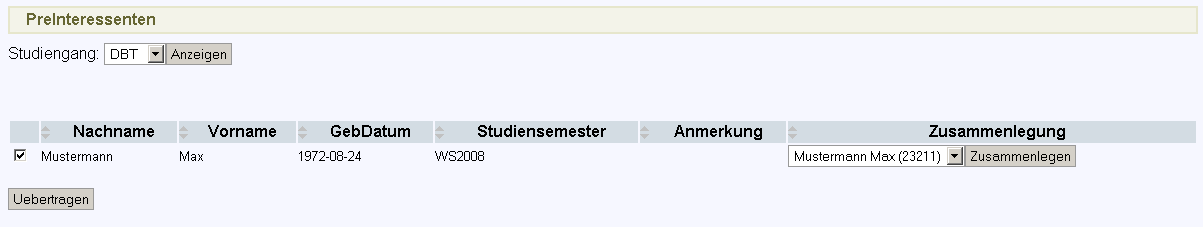
\includegraphics[width=0.75\textwidth]{FAS_Preinteressent1.png}
	\caption{Preinteressent �bernahme}
	\label{Preinteressent �bernahme}
\end{figure}
  \item Interessent existiert nicht im Studiengang\\
		Wenn die zu �bernehmende Person noch nicht im Studiengang existiert, dann wird diese einfach dadurch ins System �bertragen indem man das Hackerl vor dem Nachnamen markiert und danach auf �bertragen klickt.\\
\end{itemize}
Die Person wird nun im FAS als Interessent gef�hrt.\\

Um nach der �bertragung die Anmerkungen zu diesem Preinteressenten anzuzeigen, klicken Sie mit der rechten Maustaste auf den Interessenten und w�hlen den Men�punkt Personendetails anzeigen.
\section{Status�nderungen}
\subsection{Manuelle �nderung des Status}
\label{ManuellerStatus}
\begin{figure}
	\centering
	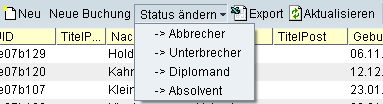
\includegraphics[width=0.75\textwidth]{FAS_Statusaendern1.png}
	\caption{Studentenstatus �ndern}
	\label{Stataend1}
\end{figure}
Eine Status�nderung durch den Anwender wird wie folgt durchgef�hrt:
\begin{itemize}
	\item Markieren der Person
	\item Anklicken des Button \textsl{Status �ndern} wie in Abbildung \ref{Stataend1} gezeigt. Der Inhalt des Auswahlfelds ist vom aktuellen Status der Person abh�ngig, da nur die Stati angezeigt werden, die vom aktuellen Status aus erreichbar sind.
	\item Auswahl des neuen Status. Es wird \underline{nur} der Status des Studenten eingetragen, es wird keine �nderung z.B. bei den Gruppenzuordnungen gemacht.
\end{itemize}
Die Inskription eines Studenten ist die Status�nderung eines Aufgenommenen auf Student. W�hren diesem Vorgang werden das Personenkennzeichen und die UID des neuen Studenten generiert.\\

\achtung{\textbf{Wichtig} Die Inskription erfolgt im gleichen Semester wie der letzte Bewerbereintrag!}\\

\underline{Beispiel}:\\
Der Student XY hat sich f�r das Wintersemester 2006 beworben und wurde am 12.06.2006 als Bewerber f�r das 3.Semester eingetragen. Im Sommer �berlegt er es sich anders und will erst im Sommersemester, dann allerdings ins 2.Semester einsteigen. Um diesen Studenten korrekt inskribieren zu k�nnen, mu� ein Bewerbereintrag und ein Aufgenommereintrag f�r das 2.Semester im Sommersemester angelegt werden. Erst danach wird der Status mit \textit{Status �ndern} auf Student gesetzt und somit der Student inskribiert.\\

\underline{Beispiel}:\\
Student des 3.Semesters Schorsch Schlaffhih bekommt im Sommersemester 2007 einen akuten Anfall von Fr�hjahrsm�dichkeit und will sich karenzieren lassen. Dazu wird �ber \textsl{Status �ndern} --- \textsl{Unterbrecher} der neue Status Unterbrecher im Sommersemester 2007 und Ausbildungssemester 3 eingetragen. Danach wird in der  Karteikarte \textsl{Details} Semester auf 0, Verband auf B (f�r Unterbrecher) und Gruppe leer gesetzt und mit der Taste \textsl{Speichern} in die Datenbank geschrieben. Bei der n�chsten Vorr�ckung wird dann der Status Unterbrecher im 3.Semester des Wintersemester 2007 gesetzt, der Unterbrecher selbst bleibt aber in der Gruppe 0B.\\
\subsection{Vorr�ckung}
Siehe Kapitel \ref{vorrueckung}.Vorr�ckung
\subsection{Korrekturm�glichkeiten}
\achtung{\textbf{Wichtig} Die Korrekturm�glichkeiten sollten nur in Ausnahmef�llen verwendet werden. Die Status�nderung, wie unter \ref{ManuellerStatus} beschrieben, ist die Standardmethode zum �ndern des Status!}\\

Kickt man eine Statuseintragung mit der rechten Maustaste an, erscheint die in Abbildung \ref{Stataend2} gezeigte Auswahl: 
\begin{itemize}
	\item Bearbeiten: Es kann f�r den ausgew�hlten Eintrag das Studiensemester, das Ausbildungssemester und das Datum der Eintragung ge�ndert werden. Der Status des Studenten kann nicht ver�ndert werden.
	\item Neuen Status hinzuf�gen: Hier kann eine neuer Status hinzugef�gt werden. Eingegeben werden mu� das Studiensemester, das Ausbildungssemester, das Datum der Eintragung (Vorgabe ist das aktuelle Datum) und der Status. Beim Status stehen nur bereits vergebene Stati zur Auswahl.
	\item Entfernen: Hier kann der ausgew�hlte Status mit Ausnahme des Status \textit{Student}, der nur vom Administrator entfernt werden kann, gel�scht werden. 
\end{itemize}
\begin{figure}
	\centering
	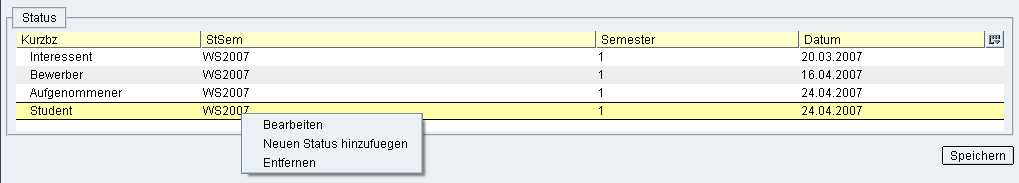
\includegraphics[width=0.75\textwidth]{FAS_Statusaendern2.png}
	\caption{Studentenstatus �ndern}
	\label{Stataend2}
\end{figure}
\section{Auslandsaufenthalt (Outgoing)}
\label{Outgoing}
Es besteht die M�glichkeit, w�hrend eines Studiums ein oder auch mehrere Semester im Ausland zu absolvieren (siehe auch Incoming \textit{Kapitel \ref{Incoming}}).\\
Dazu m�ssen folgende Daten eingegeben werden:
\begin{itemize}
	\item BIS: Daten f�r die BIS-Meldung
	\begin{itemize}
		\item Von: Beginndatum des Auslandssemesters.
		\item Bis: Endedatum des Auslandssemesters.
		\item Mobilitaetsprogramm: Hier kann das vom Studenten in Anspruch genommene Mobilit�tsprogramm ausgew�hlt werden.
		\item Gastnation: Nation in der das Auslandssemester absolviert wird. Darf nicht \textsl{�sterreich} sein.
		\item Zweck: Der Grund des Auslandsaufenthalts: Studium, Praktikum oder beides.
	\end{itemize}
	\item Outgoing(Zeugnis): Wenn f�r einen Auslandsaufenthalt eine globale Anrechnung mittels eines Eintrags im Zeugnis erfolgen soll, m�ssen nachfolgende Daten eingegeben werden. Es besteht auch weiterhin die M�glichkeit, alternativ dazu, die Lehrveranstaltungen, die urspr�nglich ohne Outgoing besucht worden w�ren, mit der Note angerechnet zu werten.
	\begin{itemize}
		\item Lehrveranstaltung: Lehrveranstaltung, die nur f�r den Auslandsaufenthalt angelegt wird. Diese LV scheint mit den Infos des Auslandaufenthalts (Zeit und Ort) am Zeugnis auf. (Bei der Lehrveranstaltung muss das Attribut lehrevz gesetzt sein, damit diese in der Liste aufscheint!)
		\item Lehreinheit: Es mu� auch eine Lehreinheit angelegt werden, der die Outgoingstudenten �ber eine Gruppe zugeordnet sind.
		\item Ort: Ort des Auslandsaufenthalts
		\item Universitaet: Name der Universit�t oder FH des Auslandsaufenthalts.
	\end{itemize}
\end{itemize}
\achtung{\textbf{Wichtig} Outgoing m�ssen in die Gruppe 0O verschoben werden, damit die Lehrveranstaltungen des gesamten Semesters nicht auf seinem Zeugnis aufscheinen und der Outgoing nicht auf den Anwesenheitslisten dieser Lehrveranstaltungen gef�hrt wird!}\\

\underline{Beispiel:}\\
Studentin XX macht ein Aulandssemester in Italien w�hrend ihres 3.Semesters. \\Eingetragen wird wie folgt:
\begin{enumerate}
	\item Vor der Eingabe der Daten des Bereichs \textit{Outgoing (Zeugnis)} mu� eine Lehrveranstaltung mit den ben�tigten ECTS-Punkten und Semesterstunden angelegt sein bzw. werden. Ist die LV vorhanden, wird im Semester des Auslandsaufenthalts dazu eine Lehreinheit angelegt. Dieser Lehreinheit werden dann �ber eine Gruppe die Outgoing-Studenten zugewiesen. Die Note f�r das Auslandssemester (meistens \textsl{angerechnet}) wird wie bei jeder \textit{gew�hnlichen} Lehrveranstaltung eingegeben.
	\item In der Karteikarte \textit{In/Out} wird durch Dr�cken der Taste \textit{Neu} die Eingabe begonnen. Im Bereich \textsl{BIS} werden das Beginn- und Endedatum, das Mobilit�tsprogramm, die Gastnation und der Zweck des Auslandssemesters eingegeben.
	\item Die genannte Lehrveranstaltung und die Lehreinheit werden dann im Karteireiter \textit{In/Out} im Bereich \textit{Outgoing (Zeugnis)} ausgew�hlt. Danach werden dann noch der Ort und der Name der Bildungseinrichtung angegeben.
	\item Die Lehrverbandsgruppe im Karteireiter \textit{Details} auf 0O �ndern.
	\item Sollten neben dem Auslandsaufenthalt auch FH-eigene Lehrveranstaltungen absolviert werden, wird der Outgoing in eine Untergruppe von 0O verschoben und diese Gruppe einer Lehreinheit der gew�nschten Lehrveranstaltung zugeordnet.
\end{enumerate}
Am Zeugnis:\\
Der Name der ausgew�hlten Lehrveranstaltung wird durch folgenden Text ersetzt:\\
Auslandsaaufenthalt: \textsc{Von}-\textsl{Bis}, \textsl{Ort},\\
\textsl{Universitaet}\\

Die im Ausland absolvierten Lehrveranstaltungen\\
werden f�r das \textsc{Sem. d. Lehreinh.} des Studiums an der\\
Fachhochschule Technikum Wien angerechnet\\
(Details siehe Transscript of Records der\\
Gasthochschule).\\
Note, Anzahl der SWS und die ECTS-Punkte werden von der Lehrveranstaltung ins Zeugnis �bernommen.
Sollte die Studentin XX noch weitere Lehrveranstaltungen besucht haben, k�nnen diese wie gewohnt eingetragen werden. Diese Lehrveranstaltungen werden dann gemeinsam mit der Anrechnung des Auslandssemesters am Zeugnis aufscheinen.
\begin{figure}
	\centering
	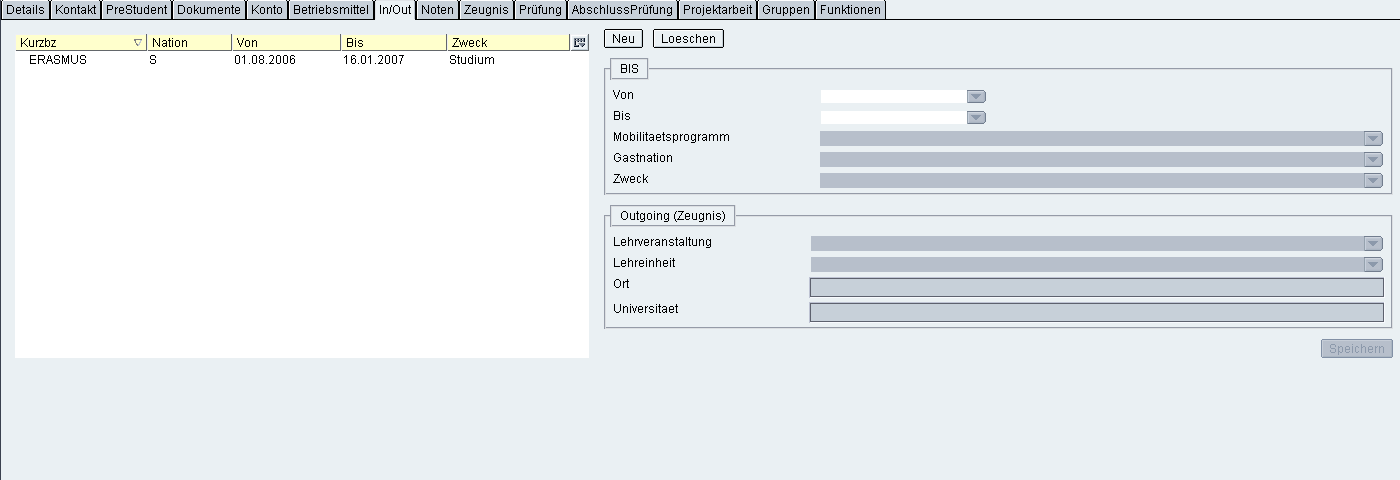
\includegraphics[width=0.75\textwidth]{FAS_IO.png}
	\caption{Die Karteikarte I/O}
	\label{IO2}
\end{figure}
\section{Gruppen}
\label{gruppen}
Im FAS gibt es zwei Arten von Studentengruppen - Lehrverbandsgruppen und Spezialgruppen. Alle Gruppen werden vom Administrator angelegt.
\subsection{Lehrverbandsgruppen}
Lehrverbandsgruppen sind maximal 3-stufig und bilden die Grundlage der Unterrichtsplanung indem die Studenten eines Jahrgangs je nach Anzahl in kleinere Teile gegliedert werden:
\begin{enumerate}
	\item Semester: Zum einen ist der erste Teil das Semester, in dem sich der Student befindet, zum anderen kann aber auch eine Organisationseinheit verwendet werden, wie das Semester 0 f�r Abbrecher (0A), Unterbrecher (0B), Incoming (0I) und Outgoing (0O). 
	\item Lehrverband: Unterteilung des Semesters in mehrere Teile und wird beginnend mit A mit Gro�buchstaben benannt.
	\item Gruppe: Weiter Unterteilung der Lehrverb�nder in Gruppen. Bezeichnungen sind Zahlen beginnend mit 1.
\end{enumerate}
Jeder Student mu� genau einer Lehrverbandsgruppe zugeordnet werden. Die Zuordnung der Studenten zu einer Lehrverbandsgruppe erfolgt durch einen Eintrag in der Kateikarte \textsl{Details} unter \textsl{Student}.
\subsection{Spezialgruppen}
Spezialgruppen sind das organisatorische Bindeglied zwischen Studenten und Lehrveranstaltungen, die au�erhalb der Lehrverbandsstrukturen zugeteilt werden (z.B.: Wahlf�cher).\\
\underline{Beispiel:}\\
Der Studiengang 1 bietet ein Wahlfach XY an. Da dieses Wahlfach von den verschiedensten Studenten besucht werden kann, die sich nicht in einer Lehrverbandsgruppe, ja nicht einmal im selben Studiengang befinden, mu� f�r diese Lehrveranstaltung eine eigene Spezialgruppe angelegt werden. Die Zuordnung der Studenten erfolgt mittels Drag \& Drop - die Studenten werden mit der Maus vom Listenfenster in die Gruppe im linken Fenster auf die entsprechende Gruppe gezogen. Sollte ein Student aus einem anderen Studiengang teilnehmen wollen, mu� er mit der Personensuche aufgelistet werden und dann in die Gruppe gezogen werden.
\section{Rechtsklickfunktionen}
\begin{itemize}
	\item \textsl{Student aus Gruppe entfernen}: (auch m�glich, wenn mehrere Studenten markiert wurden) entfernt den Studenten aus einer Spezialgruppe. Dazu muss im linken Men� eine Spezialgruppe ausgew�hlt sein. Aus Lehrverbandsgruppen k�nnen die Personen auf diese Art nicht entfernt werden.
	\item \textsl{E-Mail senden}: Es wird ein E-Mail Fenster ge�ffnet, bei dem die markierten Studenten als Empf�nger eingetragen sind.\\
	Wird der Eintrag 'E-Mail senden (intern)' gew�hlt werden die Adressen der Hochschule eingetragen.\\
	Wenn der Eintrag 'E-Mail senden (privat)' gew�hlt wird, dann wird das E-Mail an die Zustell-E-Mail-Adresse gesendet die unter Kontakt eingetragen wurde.\\
	\\
	Aus technischen Gr�nden ist die maximale Anzahl an Empf�ngern pro E-Mail begrenzt. Wenn diese Grenze �berschritten wird, wird automatisch ein 2. E-Mail Fenster mit den restlichen Empf�ngern ge�ffnet.
	\item \textsl{Personendetails anzeigen}: zeigt eine Gesamt�bersicht �ber die Person an (Wo hat er sich nicht beworben, In welchen Studieng�ngen studiert diese Person noch,...)
\end{itemize}
\chapter{Stammdaten}
\label{details}
\section{Die Karteikarte Details}
\begin{figure}
	\centering
	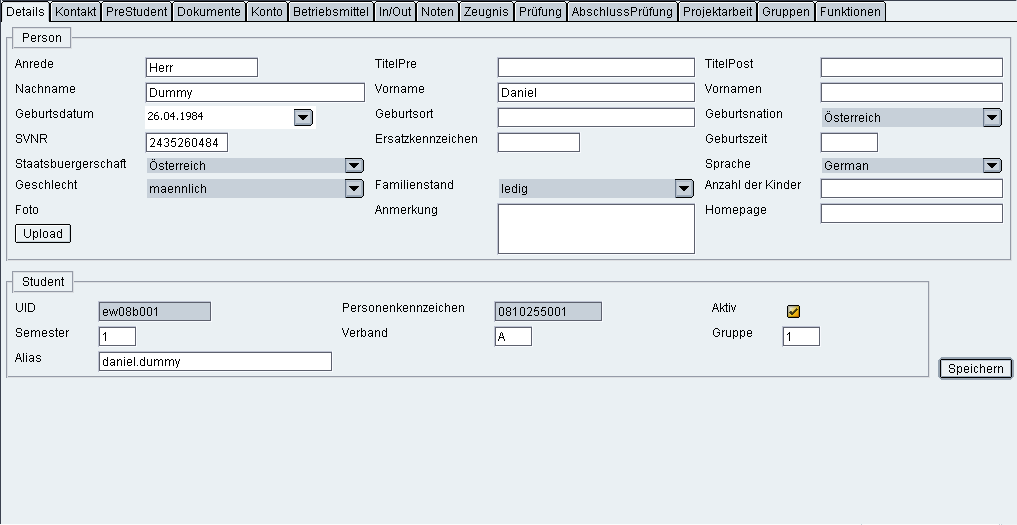
\includegraphics[width=0.75\textwidth]{FAS_Details1.png}
	\caption{Die Karteikarte Details}
	\label{Details1}
\end{figure}
\begin{itemize}
	\item Bereich Person:
	\begin{itemize}
		\item Anrede: Die Anrede der Person findet Verwendung in Ausdrucken wie etwa in Briefk�pfen.
		\item TitelPre: Akademische Titel, die \textbf{vor} dem Name gef�hrt werden. (Um ein hochgestelltes 'a' zu erzeugen halten Sie die <Alt>-Taste gedr�ckt und tippen sie 0170 am Ziffernblick der Tastatur. z.B. f�r Mag�)
		\item TitelPost: Akademische Titel, die \textbf{nach} dem Name gef�hrt werden.
		\item Nachname: Nachname der Person.
		\item Vorname: Vorname der Person.
		\item Vornamen: Weitere Vornamen der Person.
		\item Geburtsdatum: Das Geburtsdatum wird als Entscheidungskriterium f�r die Zusammenlegung von Personendatens�tzen herangezogen, wenn die Sozialversicherung noch nicht eingegeben ist wie es z.B. bei Interessenten vorkommt. Eine Zusammenlegung von Personendatens�tzen wird vorgenommen, damit eine Person nur einmal in der Datenbank abgebildet ist und Redundanzprobleme vermieden werden.
		\item Geburtsort
		\item Geburtsnation
		\item SVNR: Die Sozialversicherungsnummer wird haupts�chlich f�r die BIS-Meldung ben�tigt.
		\item Ersatzkennzeichen: Das Ersatzkennzeichen ist eine Ersatznummer f�r die Sozialversicherungsnummer als �bergangsl�sung bis die Sozialversicherungsnummer vergeben wurde.
		\item Geburtszeit 
		\item Staatsb�rgerschaft: Die Staatsb�rgerschaft wird f�r die BIS-Meldung ben�tigt.
		\item Sprache
		\item Geschlecht 
		\item Familienstand
		\item Anzahl der Kinder
		\item Foto: Die Taste \textsl{Upload} startet einen Dialog zum Einf�gen eines Bildes der Person.
		\item Anmerkung: Hier k�nnen zus�tzliche Informationen eingegeben werden.
		\item Homepage: URL einer Homepage der Person.
	\end{itemize}
	\item Bereich Student:
	\begin{itemize}
		\item UID: Wird bei der Inskription automatisch vergeben, wird vom Personenkennzeichen abgeleitet.
		\item Personenkennzeichen: Eindeutige Identifikationsnummer f�r Studenten. Wird ebenfalls bei der Inskription automatisch vergeben. \\
		Aufbau:
	\begin{itemize}
		\item 2-stellige Jahreszahl der Inskription.
		\item Semesterkennung: 1 f�r WS, 2 f�r SS, 0 f�r Incomingstudenten
		\item 4-stellige Studienkennzahl
		\item 3-stellige laufende Nummer 
	\end{itemize}
		\item Aktiv: Das H�kchen ist standardm��ig gesetzt und gibt an, ob diese Person aktiv studiert und somit ins n�chste Semester vorger�ckt wird oder nicht.
		\item Semester: Ausbildungssemester in dem sich der Student w�hrend des ausgew�hlten Studiensemesters befindet.
		\item Verband: Unterteilung des Ausbildungssemesters.
		\item Gruppe: Unterteilung des Verbands.
		\item Alias: Alternative Emailadresse f�r Studenten. Wird in der Regel automatisch generiert. Regeln: Der Aufbau mu� nach dem Schema \textsl{vorname.nachname} ohne Umlaute erfolgen. Vorname und Nachname m�ssen zumindest je einen Buchstaben lang sein. \textsl{@technikum-wien.at} wird automatisch hinzugef�gt.
	\end{itemize}
\end{itemize}
\newpage
\label{pflichtstamm}
\section{Pflichtfelder}
\begin{figure}
	\centering
	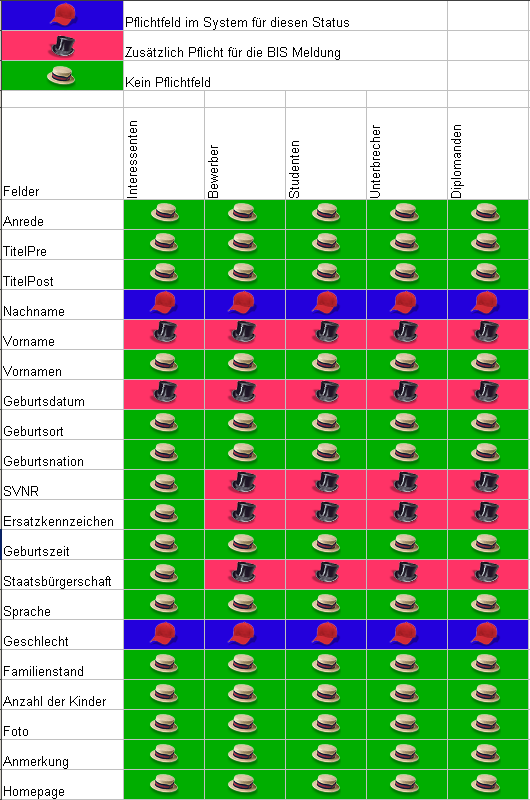
\includegraphics[width=0.75\textwidth]{FAS_Pflichtfelder_Stammdaten.png}
	\caption{Die Pflichtfelder des Karteireiters Stammdaten}
	\label{Bild_Pflichtstamm}
\end{figure}

\chapter{Prestudent}
\label{prestudent}
\section{Aufbau der Karteikarte Prestudent}
\begin{figure}
	\centering
	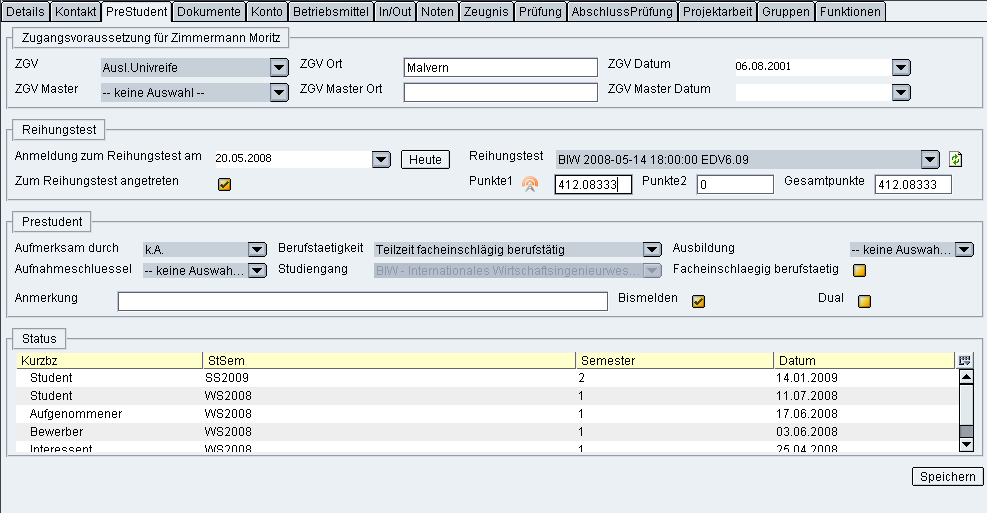
\includegraphics[width=0.75\textwidth]{FAS_Prestudent1.png}
	\caption{Die Karteikarte Prestudent}
	\label{Prestudent1}
\end{figure}
\begin{itemize}
	\item Zugangsvoraussetzungen: 	
	\begin{itemize}
		\item ZGV: Zugangsvoraussetzungen, die zu einer Teilnahme an einem Diplom- oder Bachelorstudiengang berechtigt. Schultyp und Datum des Abschlu�zeugnisses sind Teil der Studenten-BIS-Meldung.
		\item ZGV Master: Zugangsvoraussetzung, die zu einer Reilnahme an einem Masterstudiengang berechtigen.
	\end{itemize}
\achtung{\textbf{Wichtig} Die BIS-Meldung verlangt in Masterstudieng�ngen die Eintragung beider Zugangsvorraussetzungen!}\\

\idee{\textbf{Tipp} Bei Interessenten, die ihren Abschlu� noch nicht gemacht haben, sollte f�r die Interessentenstatistik die ZGV m�glichst fr�h bereits eingegeben werden! Das ZGV-Datum wird dann nach der bestandenen Pr�fung eingetragen.}\\

	\item Reihungstest: 
	\begin{itemize}
		\item Anmeldung zum Reihungstest am: Hier kann das Datum der Anmeldung zum Reihungstest eingegeben oder mit dem Kalendertool ausgew�hlt werden. Die rechts vom Eingabefeld befindliche Taste \textit{Heute} setzt das aktuelle Datum in das Eingabefeld. Bei der Inskription mu� das Datum eingegeben sein.
		\item Reihungstest: Auswahl des Reihungstests. Beim Speichern wird gepr�ft, ob diese Person in einem anderen Studiengang des selben Typs (Master, Bachelor,...) bereits einen Reihungstesttermin hat. Falls dies der Fall ist, wird eine Warnung angezeigt. Die Daten trotzdem gespeichert.
		Rechts neben dem Auswahlfeld befindet sich 
\includegraphics{icon_aktualisieren}, eine Aktualisierungstaste. Dieser kann verwendet werden, um die Liste zu aktualisieren, wenn ein neuer Reihungstesttermin �ber die Reihungstestverwaltung angelegt wird.
		\item Zum Reihungstest angetreten: Zeigt an, ob der Bewerber zu einem Reihungstest angetreten ist. Bei aktiven Studenten mu� das H�kchen gesetzt sein (BIS-Meldung).
		\item Reihungstestpunkte: Die Reihungstestpunkte sind in 3 Felder unterteilt. Das Feld Punkte1 sind die Punkte des elektronischen Reihungstests. Die Punkte des Testtools k�nnen automatisch �bernommen werden wenn auf das Symbol neben dem Eingabefeld geklickt wird. (Die Punkte aus dem Dynamic Power Trainer k�nnen hier nicht automatisch �bernommen werden.) Das Feld Punkte2 enth�lt die Punkte des Pers�nlichen Gespr�chs bzw weitere Aufnahmekriterien (Sporttest). Das 3. Feld enth�lt die Gesamtpunkte. Diese werden in der Regel automatisch aus den beiden anderen Feldern berechnet. 
	\end{itemize}
	\item Prestudent:
	\begin{itemize}
		\item Aufmerksam durch: Auswahl, wodurch der Student auf den Studiengang aufmerksam wurde. 
		\item Berufstaetigkeit: 
		\item Ausbildung: Eingabe der h�chsten abgeschlossenen Ausbildung.
		\item Aufnahmeschluessel
		\item Studiengang: Zeigt den Studiengang an.
		\item Facheinschlaegig berufstaetig: 
		\item Anmerkung: Hier k�nnen zus�tzliche Informationen eingegeben werden.
		\item Bismelden: Bestimmt, ob Student in die BIS-Meldung gelangt. Das H�kchen ist standardm��ig gesetzt.\\
		\underline{Beispiel}:\\
		Student XY inskribiert im Juni das n�chste Wintersemester im Studiengang YZ. Am 17.Oktober gibt der Student aber das Studium auf. Vorgehensweise: Der Status des Studenten wird auf \textsl{Abbrecher} gesetzt. Danach wird das \textsl{Aktiv}-H�kchen in der Karteikarte \textit{Details} und das \textsl{Bismelden}-H�kchen entfernt. Somit wird der Student zum Abbrecher gemacht und nicht in der n�chsten BIS-Meldung am 15.November gemeldet.\\
	\end{itemize} 
	\item Status: Dieser Bereich besteht aus einer Liste aller Stati des ausgew�hlten Studenten.
\end{itemize}
\achtung{\textbf{Wichtig} Bei der BIS-Meldung d�rfen keine Studienanf�nger gemeldet werden, die vor dem Stichtag der ersten BIS-Meldung das Studium abgebrochen haben!}\\

\section{Rechtsklick-Funktionen}
Im Listenfeld \textit{Status} gibt es drei Funktionen, die mit einem Rechtsklick aufgerufen werden:
\begin{itemize}
	\item Bearbeiten: Bei einem im Listenfeld markierten Status k�nnen folgende Daten ver�ndert werden:
	\begin{itemize}
		\item Studiensemester
		\item Ausbildungssemester
		\item Datum
	\end{itemize}
	\item Neuen Status einfuegen: Hier kann dem Studenten ein neuer Status hinzugef�gt werden. \\
	Einschr�nkungen:	
	\begin{itemize}
		\item Es k�nnen nur die Stati \textit{Interessent}, \textit{Bewerber} und \textit{Student} gesetzt werden.
		\item Der Status \textit{Student} kann nur eingef�gt werden, wenn der Student bereits einen Status \textit{Student} besitzt, also schon inskribiert ist. Die Inskription erfolgt mittels \textit{Status �ndern}, wie im Kapitel \ref{ManuellerStatus} beschrieben.
		\item Es k�nnen keine zwei gleiche Stati im selben Studiensemester eingegeben werden.
	\end{itemize}
	\item Entfernen: Hier kann ein markierter Status gel�scht werden.\\
	Einschr�nkungen:
	\begin{itemize}
		\item Es k�nnen alle bis auf einen Status gel�scht werden.
		\item Studentenstati k�nnen nur vom Administrator entfernt werden.
	\end{itemize}
\end{itemize}
\newpage
\label{pflichtpre}
\section{Pflichtfelder}
\begin{figure}
	\centering
	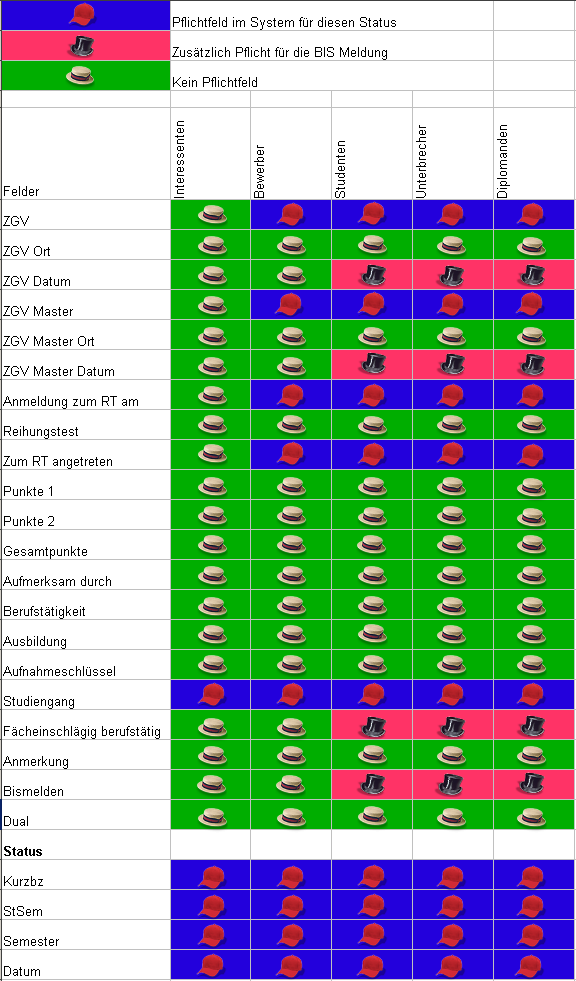
\includegraphics[width=0.70\textwidth]{FAS_Pflichtfelder_PreStudent.png}
	\caption{Die Pflichtfelder des Karteireiters Prestudent}
	\label{Bild_Pflichtpre}
\end{figure}
\chapter{Incoming}
\label{Incoming}
Als Incoming werden Studenten ausl�ndischer Fachhochschulen bezeichnet, die hier ein oder mehrere Auslandssemester absolvieren. Die BIS-Meldung schreibt vor, da� Incoming zwar bei einem Studiengang gemeldet werden m�ssen, aber in keinem Semester gemeldet werden d�rfen. Das Anlegen eines Incoming erfolgt genauso wie bei einem regul�ren Studenten (siehe Kapitel \ref{Anlegen eines neuen Interessenten} mit einem kleinen Unterschied: Wie in Abbildung \ref{Incoming1} mit 1 bezeichnet, wird der Radiobutton \textsl{Incoming} angehakt. Somit wird keine Interessentenrolle sondern eine Incomingrolle vergeben und der Incoming-Student automatisch dem Semester 0I zugeteilt. Incoming-Studenten werden dort einzeln in Untergruppen (0I1, 0I2,...) aufgeteilt. Die Untergruppe eines Incoming-Studenten wird nun einer Lehreinheit der vom Studenten ausw�hlten Lehrveranstaltung zugeordnet.
\begin{figure}
	\begin{center}
    \begin{picture}(128,86)
			\put(20,0){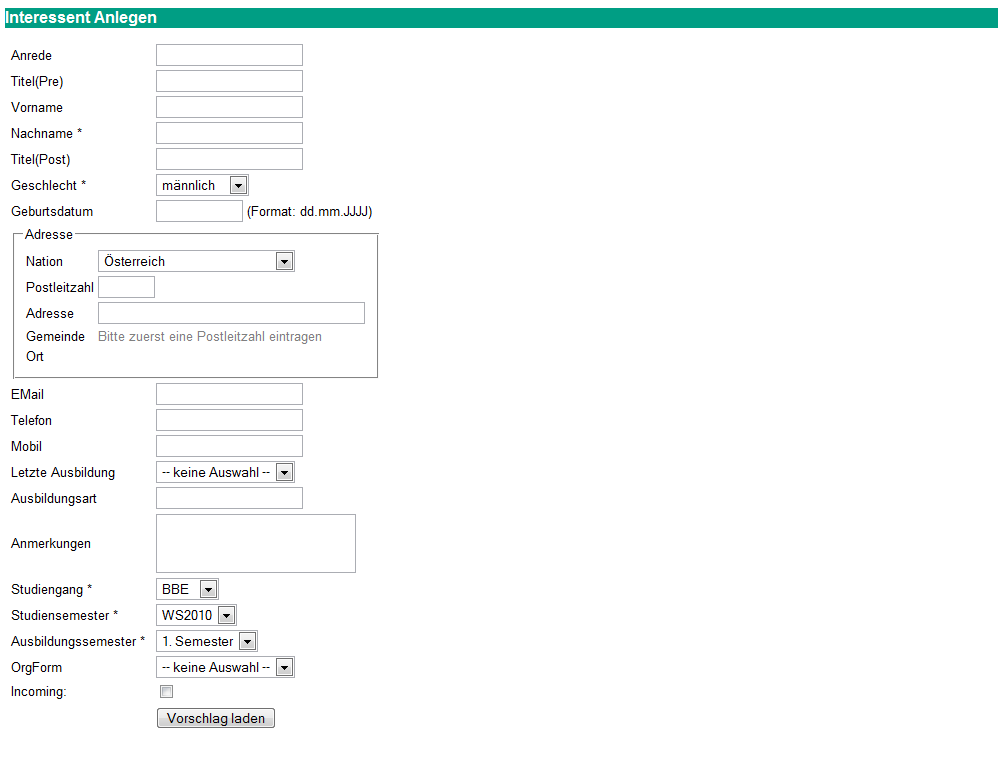
\includegraphics[height=86mm, width=128mm]{FAS_Interessent1.png}}
			\markier{1}{15}{10}{3}{-1}
		\end{picture}
    \caption{Incoming anlegen}
		\label{Incoming1}
  \end{center}
\end{figure}
Nach dem Anlegen des Incoming sollten noch dessen I/O-Daten eingegeben werden. Dazu wird die Karteikarte \textit{In/Out} des Studenten wie in Abbildung \ref{IO1} ge�ffnet:
\begin{itemize}
	\item BIS: Daten, die f�r die BIS-Meldung ben�tigt werden:
	\begin{itemize}
		\item Von: Beginn des Aufenthalts.
		\item Bis: Ende des Aufenthalts.
		\item Mobilitaetsprogramm: Hier kann das vom Studenten in Anspruch genommene Mobilit�tsprogramm ausgew�hlt werden. 
		\item Gastnation: Nation in der der Auslandsaufenthalt stattfindet, bei Incoming immer �sterreich, bei Outgoing nie.
		\item Zweck: Der Grund des Auslandsaufenthalts: Studium, Praktikum oder beides.
	\end{itemize}
	\item Der Bereich \textit{Outgoing(Zeugnis)} mu� bei Incoming-Studenten nicht ausgef�llt werden.
\end{itemize}	
\begin{figure}
	\centering
	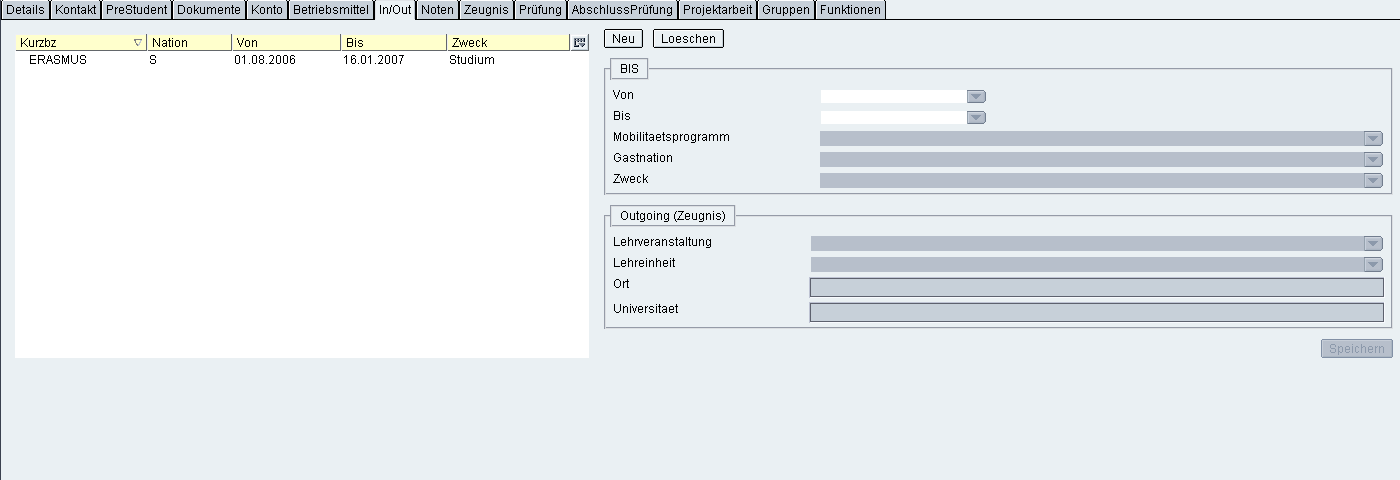
\includegraphics[width=0.75\textwidth]{FAS_IO.png}
	\caption{Die Karteikarte I/O}
	\label{IO1}
\end{figure}
Sonderf�lle:
\begin{itemize}
	\item Sollte ein Icoming trotz Anmeldung nicht zum Auslandssemester erscheinen, mu� er auch nicht BIS-gemeldet werden. Wenn der Incoming schon im FASonline eingetragen ist, kann die Meldung unterdr�ckt werden indem das H�kchen bei \textit{Bismelden} in der Karteikarte \textit{PreStudent} entfernt wird.
	\item Incoming, deren Aufenthalt keinen BIS-Meldungsstichtag einschlie�t, werden in der dem Aufenthalt nachfolgenden BIS-Meldung gemeldet.
\end{itemize}
\chapter{Kontakte}
\label{kontakte}
Die Karteikarte \textit{Kontakte} (Abbildung \ref{Kontakte1}) beinhaltet die Daten zur Kontaktaufnahme mit dem Studenten. Im oberen Feld werden die Adressen gespeichert, im mittleren Telefon- und Faxnummern sowie Emailadressen und im unteresten Feld k�nnen Bankverbindungsdaten festgehalten werden.
\begin{figure}
	\centering
	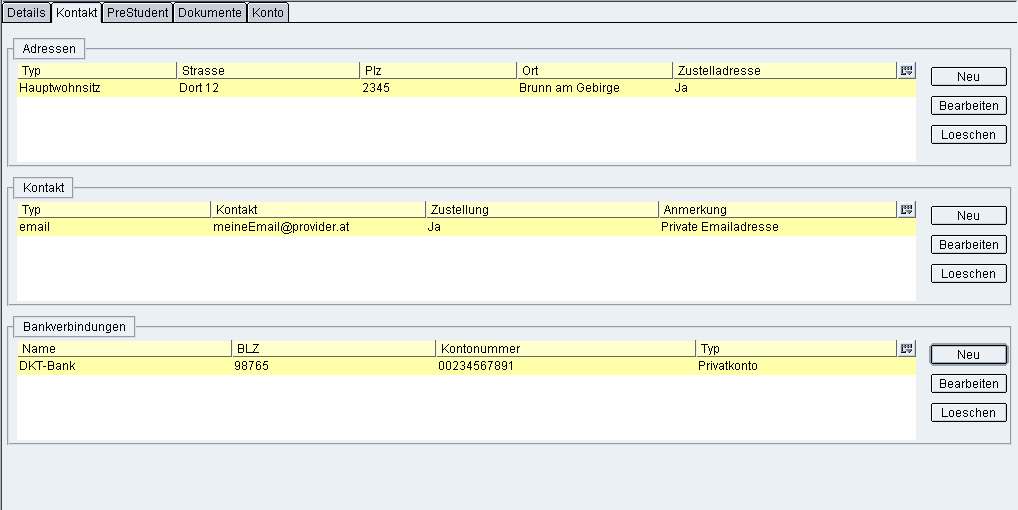
\includegraphics[width=0.75\textwidth]{FAS_Kontakte1.png}
	\caption{Die Karteikarte Kontakte}
	\label{Kontakte1}
\end{figure}
\section{Anlegen von Adressen}
Das Feld \textsl{Adressen} besteht aus einer Liste sowie drei Tasten. Durch Dr�cken der Taste \textit{Neu} kann eine Adresse hinzugef�gt werden. Es wird die Eingabemaske wie in Abbildung \ref{Kontakte2} ge�ffnet. Die Eingabemaske besteht aus folgenden Teilen:
\begin{itemize}
	\item Typ: Hier wird ausgew�hlt, um welchen Adresstyp es sich bei der Eintragung handelt. Zur Auswahl stehen Hauptwohnsitz, Nebenwohnsitz und Firma f�r eine Firmenanschrift.
	\item Strasse: Strassen- oder Gassenname der Adresse.
	\item Nation: Gibt an in welchem Land die Adresse sich befindet. Wird hier �sterreich angegeben, wird in den folgenden Auswahlfeldern die Postleitzahlentabelle des FHR verwendet.
	\item Plz: Die Postleitzahl der Adresse.
	\item Gemeinde: Handelt es sich um eine �sterreichische Adresse, mu� der Gemeindename in der Liste des FHR vorkommen, ansonsten kann der Gemeindename frei eingegeben werden.
	\item Ortschaft: Handelt es sich um eine �sterreichische Adresse, mu� der Ortschaftsname aus der Liste des FHR ausgew�hlt werden, ansonsten kann der Gemeindename frei eingegeben werden.
	\item Heimatadresse: Kennzeichnet diese Adresse als Heimatadresse. Das ist jene Adresse, die zum Zeitpunkt der Inskription der Hauptwohnsitz des Studenten war. \\
\end{itemize}
\achtung{\textbf{Wichtig} Die Heimatadresse darf sich w�hrend eines Studiums nicht ver�ndern!\\
	(BIS-Meldung) Wenn das Attribut Heimatadresse gesetzt ist, kann diese Adresse daher nicht gel�scht werden. Um diese Adresse dennoch zu l�schen muss erst das Hackerl bei Heimatadresse entfernt werden.}\\

\begin{itemize}
	\item Zustelladresse: Postalische Zustellungen an desn Studenten sollen zu dieser Adresse erfolgen.
	\item Firma: Hier kann die Firma ausgew�hlt werden zu der diese Adresse geh�rt. Tippen Sie dazu in das Feld den Namen der Firma ein. Danach werden in dem DropDown Feld die Firmen angezeigt die diesem Suchkriterium entsprechen. (Es m�ssen mindestens 3 Zeichen eingegeben werden damit die Eintr�ge angezeigt werden.
	\item Anmerkung: Hier k�nnen zus�tzliche Informationen eingegeben werden.\\
\end{itemize}
\achtung{\textbf{Wichtig} Erst durch Dr�cken der Taste \textsl{Speichern} werden die Daten in die Datenbank �bertragen! Wird das Eingabeformular vor dem Dr�cken der Taste \textsl{Speichern} geschlossen, werden die Daten verworfen.}\\

Durch Dr�cken der Taste \textit{Bearbeiten} kann eine zuvor ausgew�hlte Adresse ge�ndert werden. Es �ffnet sich hier die selbe Eingabemaske bereits vorbef�llt mit den gespeicherten Daten. Die Daten k�nnen nun ver�ndert und mittels \textsl{Speichern}-Taste in die Datenbank �bertragen werden.
Mit der Taste \textsl{Loeschen} kann ein ausgew�hlter Eintrag entfernt werden.
\begin{figure}
	\centering
	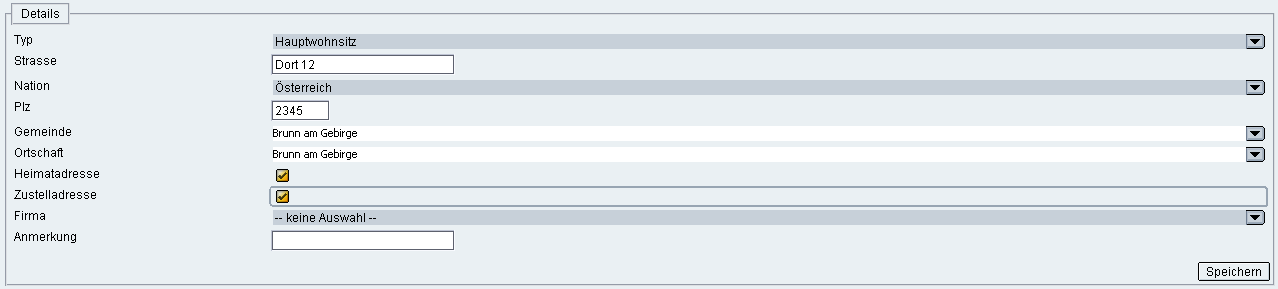
\includegraphics[width=0.75\textwidth]{FAS_Kontakte2.png}
	\caption{Adressen anlegen}
	\label{Kontakte2}
\end{figure}
\section{Anlegen von Kontaktm�glichkeiten}
Das Feld \textsl{Kontakte} gleicht in Aufbau und Funktion dem zuvor beschriebenen Feld \textsl{Adressen}. Die Eingabemaske besteht hier allerdings aus folgenden Teilen:
\begin{itemize}
	\item Typ: Hier wird der Kontakttyp festgelegt. Zur Auswahl stehen E-Mail, Faxnummer, Mobiltelefonnummer, sonstige Telefonnummer und Telefonnummer.
	\item Kontakt: Passend zum Kontakttyp wird die E-Mailadresse oder Fax- oder Telefonnummer eingegeben.
	\item Anmerkung: Hier k�nnen zus�tzliche Informationen eingegeben werden.
	\item Zustellung: Zeigt an, ob zu diesem Kontakt Mitteilungen und Infos geschickt werden sollen.  
	\item Firma/Standort: Hier kann die Firma ausgew�hlt werden zu der dieser Kontakt geh�rt. Tippen Sie dazu in das erste Feld den Namen der Firma ein (zumindest 3 Zeichen) und w�hlen Sie den entsprechenden Eintrag aus der Liste aus. Im zweiten Feld werden dann die zugeh�rigen Standorte dieser Firma angezeigt. W�hlen Sie auch hier einen der Eintr�ge aus.
\end{itemize}
\begin{figure}
	\centering
	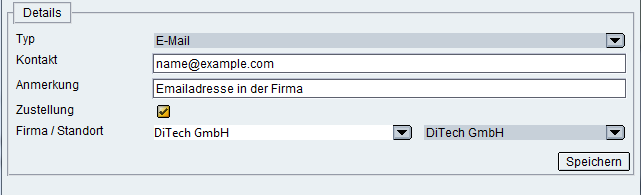
\includegraphics[width=0.75\textwidth]{FAS_Kontakte3.png}
	\caption{Kontaktm�glichkeiten anlegen am Beispiel einer E-Mailadresse}
	\label{Kontakte3}
\end{figure}
\section{Anlegen von Bankverbindungen}
Auch das Feld \textsl{Bankverbindungen}  gleicht im Aufbau und Funktion den zuvor beschriebenen Feldern. Die Eingabemaske beinhaltet folgende Eingabefenster:
\begin{itemize}
	\item Name: Eingabefeld f�r den Namen der Bank.
	\item Anschrift: Hier wird die Adresse der Bank eingegeben.
	\item BIC: Der SWIFT-BIC (SWIFT ist die Abk�rzung f�r \textbf{S}ociety for \textbf{W}orldwide \textbf{I}nterbank \textbf{F}inancial \textbf{T}elecommunication, BIC ist die Abk�rzung f�r \textbf{B}ank \textbf{I}dentifier \textbf{C}ode) ist ein nach ISO 9362 international standardisierten Bankcode, mit dem weltweit jedes direkt oder indirekt teilnehmende Kreditinstitut eindeutig identifiziert werden kann. Er findet weltweit Verwendung bei grenz�berschreitenden Zahlungen und beim \textbf{internationalen} Austausch von Nachrichten zwischen Kreditinstituten. \\
Der BIC oder SWIFT-Code hat eine L�nge von 8 oder 11 alphanumerischen Zeichen und folgenden Aufbau:\\

 BBBBCCLLbbb\\
 
\begin{itemize}
	\item BBBB  4-stelliger Bankcode, vom Geldinstitut frei w�hlbar (nur Alphazeichen)
	\item CC    2-stelliger L�ndercode nach ISO 3166-1 (nur Alphazeichen)
	\item LL    2-stellige Codierung des Ortes (alphanumerische Zeichen; wenn das zweite
       Zeichen eine 1 ist, so handelt es sich um einen passiven SWIFT-Teilnehmer)
	\item bbb   3-stellige Kennzeichnung der Filiale oder Abteilung (optional, 
       Standard: "XXX", kann weggelassen werden, andere Kennzeichen nicht)
       (alphanumerische Zeichen)
\end{itemize}
(http://de.wikipedia.org/wiki/SWIFT, 04.01.2008)
	\item BLZ: Die Bankleitzahl (BLZ) ist in Deutschland und �sterreich eine Kennziffer zur eindeutigen Identifizierung eines Kreditinstituts. Die Bankleitzahl besteht in Deutschland immer aus acht Ziffern, in �sterreich aus f�nf Ziffern. In der Schweiz und in Liechtenstein hat die Bankenclearing-Nummer (BC-Nummer) dieselbe Bedeutung.\\
(http://de.wikipedia.org/wiki/Bankleitzahl, 04.01.2008)\\
Die Bankleitzahl ist nur f�r innerstaatliche �berweisungen wichtig, f�r �berweisungen in der EU oder in Drittstaaten sollten BIC und IBAN verwendet werden.
	\item IBAN: Die \textbf{I}nternational \textbf{B}ank \textbf{A}ccount \textbf{N}umber (IBAN) ist eine internationale, standardisierte Notation f�r Bankkontonummern. Die Notation wird durch die ISO-Norm ISO 13616:2003 beschrieben. \\
	IBAN-Struktur in verschiedenen L�ndern:\\
	\begin{table*}[htbp]
	\centering
			\begin{tabular}{lcl}
Land&Stellen&Struktur\\
\hline
Oesterreich&20&ATpp bbbb bkkk kkkk kkkk\\
Deutschland&22&DEpp bbbb bbbb kkkk kkkk kk\\
Italien&27&ITpp ABBB BBCC CCCX XXXX XXXX XXX\\
Malta&31&MTpp bbbb ssss skkk kkkk kkkk kkkk kkk\\
...\\
			\end{tabular}
		\caption{IBAN-Strukturen}
		\label{tab:IBAN-Strukturen}
	\end{table*}
		
Dabei bedeutet:
	\begin{itemize}
		\item AT, DE...    L�nderkennzeichen
		\item pp           zweistellige Pr�fziffer
		\item b            Stelle der Bankleitzahl
		\item d            Kontotyp
		\item g            code guichet
		\item k            Stelle der Kontonummer
		\item K            Kontrollziffer
		\item r            Regionalcode
		\item s            Stelle des Bankcodes
		\item A,B,C,X      sonstige Funktionen
	\end{itemize}
	
K�rzere Kontonummern werden mit f�hrenden Nullen auf 10 Stellen erweitert.\\
Die IBAN kann maximal 34 Stellen umfassen und findet zur Zeit haupts�chlich beim Zahlungsverkehr innerhalb der Europ�ischen Union Verwendung. Dies gilt sowohl f�r das Datentr�geraustausch-Verfahren als auch f�r den Zahlungsverkehr mit Formularen (Zahlungsverkehrsvordrucken).\\
(http://de.wikipedia.org/wiki/International\_Bank\_Account\_Number, 04.01.2008)
	\item Kontonummer: Hier wird die Kontonummer eingegeben.
	\item Typ: Auswahl, ob es sich um ein Privat- oder Firmenkonto handelt.
	\item Verrechnungskonto: Angabe, ob es sich bei dem Eintrag um das Verrechnungskonto handelt.
\end{itemize}
\begin{figure}
	\centering
	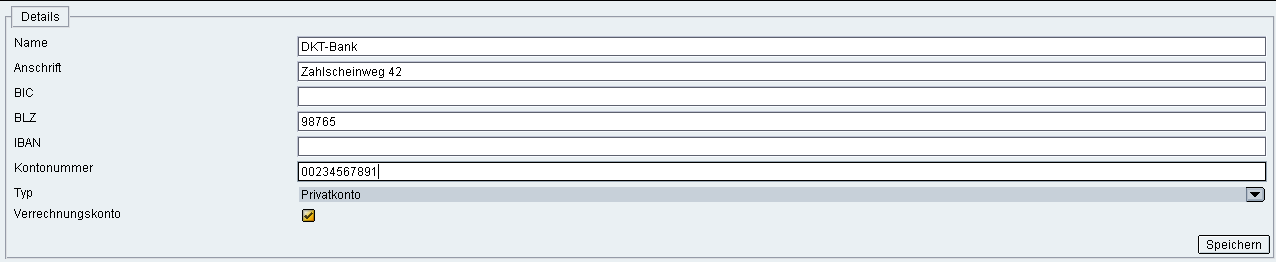
\includegraphics[width=0.75\textwidth]{FAS_Kontakte4.png}
	\caption{Bankverbindungen anlegen}
	\label{Kontakte4}
\end{figure}
\chapter{Das Studentenkonto}
\label{studentenkonto}
Das Studentenkonto dient zur Verwaltung der Ein- und Auszahlungen von bzw. an Studenten.

\section{Die Karteikarte Konto}
\begin{figure}
	\centering
	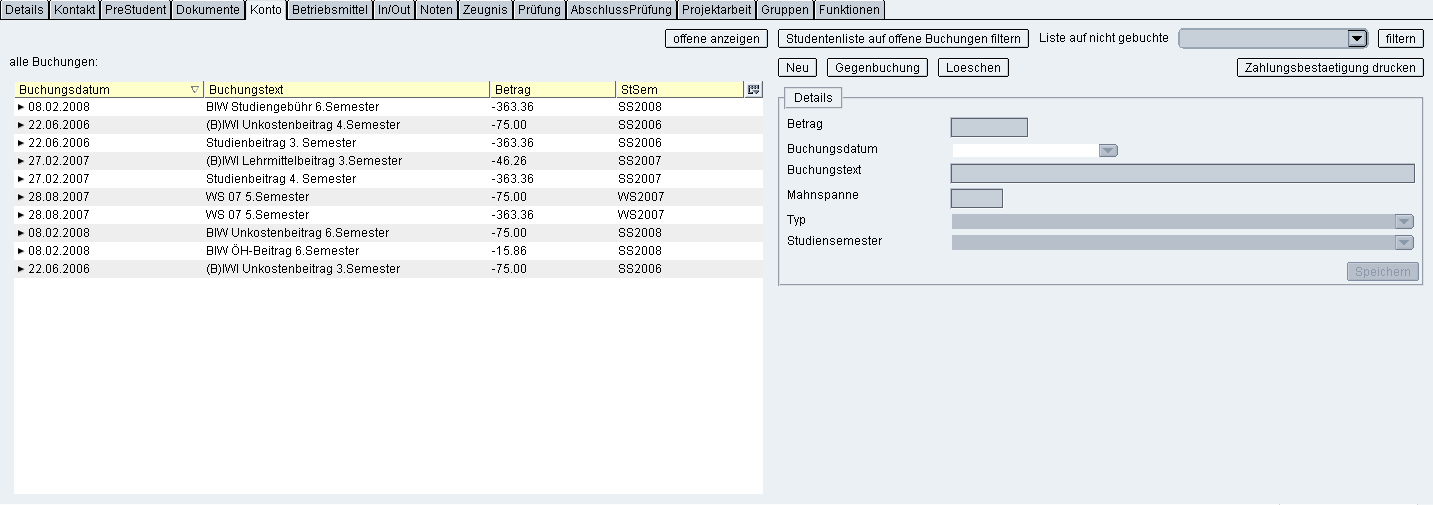
\includegraphics[width=0.75\textwidth]{FAS_Konto1.png}
	\caption{Die Karteikarte Konto}
	\label{Konto1}
\end{figure}
Die Karteikarte besteht aus folgenden Teilen (siehe Abbildung \ref{Konto1}):
\begin{itemize}
	\item Listenfeld: In diesem Anzeigefeld werden die ausgew�hlten Buchungen angezeigt.
	\item Details: Im Details-bereich k�nnen die Buchungsdaten eingegeben und ver�ndert werden.	
	\begin{itemize}
		\item Betrag: Der Buchungsbetrag wird bei einer Belastung negativ eingegeben.
		\item Buchungsdatum: Datum der Belastung oder Bezahlung.
		\item Buchungstext: Kurze Beschreibung der Buchung. (z.B.: BIF Studiengeb�hr 3.Semester)
		\item Mahnspanne: Zeitspanne in Tagen nach eine Mahnung erfolgt.
		\item Typ: Auswahl der Art der Buchung. Zur Auswahl stehen z.Z. \textsl{Kaution}, \textsl{Studiengeb�hr}, \textsl{Lehrmittelbeitrag}, \textsl{sonstiges} und \textsl{Unkostenbeitrag}
		\item Studiensemester: Das Studiensemester in dem bzw. f�r das eingezahlt oder belastet wurde.
	\end{itemize}
	\item Buttons:
	\begin{itemize}
		\item offene anzeigen/alle anzeigen: Schaltet die Anzeige im Listenfeld um. Steht auf dem Button \textsl{offene anzeigen} schaltet ein Knopfdruck auf die Anzeige der offenen Buchungen des Studenten um, steht \textsl{alle anzeigen} wird auf die Anzeige aller Buchungen geschaltet. Dadurch ergibt sich, da� auf dem Button immer das Gegenteil der zeitgleichen Anzeige im Listenfeld steht. Ob gerade alle oder nur die offenen Buchungen angezeigt werden, steht links oberhalb des Listenfelds.
		\item Liste auf nicht gebuchte (Typ) filtern: Wird der Button \textit{filtern} geklickt, werden im Listenfeld 2 alle Studenten der  Ausfwahl (z.B. Semester eines Studiengangs) aufgelistet, bei denen im ausgew�hlten Semester keine Buchung  des ausgew�hlten Typs vorhanden ist.
		\item nicht gebuchte Studiengebuehr: Liefert alle Studenten, die noch keine Belastung der Studiengeb�hr im aktuellen Semester haben.
		\item Neu: Beginn einer neuen Eintragung.
		\item Gegenbuchung: Legt eine Gegenbuchung zu einer im Listenfeld markieren Buchung an.
		\item Loeschen: Entfernen einer markieren (Gegen-)Buchung.
		\item Zahlungsbestaetigung drucken: Ausdrucken einer Zahlungsbest�tigung einer markierten Zahlung.
	\end{itemize}
\end{itemize}
\achtung{\textbf{Wichtig} Bei der Auswahl des Typs wird, sofern das \textit{Betrag}-Feld noch leer ist, dort ein default-Wert (z.B. 363.36 bei Typ Studiengeb�hr) eingef�gt. \\
Zu beachten: Da dies nur geschieht, wenn das \textit{Betrag}-Feld leer ist, wird der Betrag bei einer Fehlerkorrektur des Typs \textbf{nicht} automatisch ge�ndert, sondern mu� manuell �berschrieben werden!}\\

\info{�ber den Men�punkt Einstellungen->\textit{Buchungen auf Studiengang filtern} kann umgeschaltet werden, um alle Buchungen des Studierenden anzuzeigen bzw nur die Buchungen die den aktuellen Studiengang betreffen.}

\chapter{Vorr�ckung}
\label{vorrueckung}
Die Vorr�ckung ist die Vorbereitung auf das n�chste Studiensemester und wird nach Auftrag vom Studiengang vom Administrator durchgef�hrt. 
\section{Lehreinheiten}
Um die Planung f�r das neue Semester zu vereinfachen, k�nnen die Lehreinheiten des Vorjahres vorger�ckt werden. Dies ist speziell dann sinnvoll, wenn sich gegen�ber dem Vorjahr keine oder nur wenige �nderungen ergeben.
\section{Studenten}
Unter der Vorr�ckung der Studenten wird die Eintragung eines Status und der Lehrverbandgruppenzuteilung f�r das n�chste Studiensemester verstanden. Vorger�ckt werden nur Personen, die als \underline{aktiv} gekenntzeichnet sind.\\ 
\\
Die Vorr�ckung muss f�r jeden Studiengang jedes Semester durchgef�hrt werden, damit die Studierenden ins n�chste Semester aufsteigen.\\
Vor der durchf�hrung der Vorr�ckung sollten folgende Aktionen durchgef�hrt werden:\\
- Deaktivierung von Incoming die nicht mehr im Haus sind\\
- Status Absolvent setzen und deaktivierung von fertigen Studierenden \\
\\
Wiederholer eines Semesters werden normal vorger�ckt und nach der Vorr�ckung in das entsprechende Semester zur�ckgeschoben.\\
\\
\underline{Beispiel}:\\
Maria Musterhaft ist im Wintersemester 2006 Studentin im 1.Semester und der Gruppe 1A1 zugeteilt. Bei der Studentenvorr�ckung wird nun ein neuer Status Student im 2. Semester f�r das Sommersemester 2007 eingetragen. Weiters erfolgt eine Zuteilung der Studentin zu der Gruppe 2A1.\\
Die Semestereintragungen der Stati k�nnen nur im Bereich von 1 bis zur maximalen Semesteranzahl des Studiengangs sein (z.B. f�r Bachelorstudieng�nge sind das idR. 6 Semester). Die Semestereintragungen bei den Lehrverb�nden k�nnen auch 0 und Zahlen gr��er als die Semesterzahl sein, diese werden aber bei der Vorr�ckung dann nicht ver�ndert (z.B. wenn Unterbrecher in die Gruppe 0B verschoben wurden, befinden sich diese auch im n�chsten Semester dort).\\
\chapter{Lehrveranstaltungen}
\label{lehrveranstaltung}
Als Lehrveranstaltung wird im Gesamtsystem das gleiche verstanden, wie im Antrag des Studiengangs. Die Lehrveranstaltung wird immer aus Sicht eines Studiengangs oder aus der Sicht des Studenten gesehen. Der Titel der Lehrveranstaltung findet sich im Zeugnis und im Lehre-Bereich im CIS wieder. Nicht zu verwechseln ist die Lehrveranstaltung mit dem Lehrfach oder der Lehreinheit (siehe eigene Kapiteln).\\
Einmal verwendete Lehrveranstaltungen k�nnen nicht mehr entfernt sondern nur deaktiviert werden, da Notenzuordnungen verloren gehen w�rden.
\section{Aufbau} 
Folgende Attribute bestimmen eine Lehrveranstaltung:
\begin{table*}[htbp]
	\centering
		\begin{tabular}{|r|l|}
			\hline
			Kuerzel & Abk�rzung der LV. Mindestens 2, maximal 5 Zeichen. \\&3,4 od. 5tes Zeichen darf eine Ziffer sein.\\& Buchstaben sollten einheitlich gro� geschrieben werden.\\
			\hline
			Bezeichnung & Name der Lehrveranstaltung (max. 64 Zeichen)\\
			\hline
			LehreVz	& Der Name des Lehreverzeichnisses sollte mit dem K�rzel �bereinstimmen. 
				\\&Es sind ausschlie�lich kleingeschriebene Buchstaben zu verwenden. 
				\\&Dies legt fest, wie der Ordner der LV im Filesystem heisst. 
				\\&Wenn 2 Lehrveranstaltungen im selben Studiengang und Semester das gleiche 
				\\&Lehreverzeichnis eingetragen haben, dann wird im CIS f�r beide LVs das gleiche 
				\\&Download, Upload und Semesterplanverzeichnis verwendet.\\
			\hline
		\end{tabular}
	\caption{Attribute der Lehrveranstaltung}
	\label{tab:AttributeDerLehrveranstaltung}
\end{table*}
\section{Bearbeiten von LV-Eintr�gen}
Kommt es zu Curriculums�nderungen, stehen dem FAS-Anwender einige Anpassungsm�glichkeiten zur Verf�gung. Der Aufruf erfolgt durch Anklicken von Men�punkt \textit{Lehrveranstaltungsverwaltung} unter \textsl{Extras} wie Abbildung \ref{LV} zeigt.
\begin{figure}
	\centering
	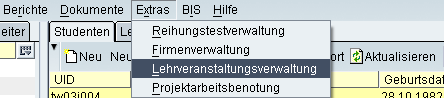
\includegraphics[width=0.75\textwidth]{FAS_LV.png}
	\caption{Bearbeiten von Lehrveranstaltungseintr�gen}
	\label{LV}
\end{figure}
Der Anwender gelangt daraufhin auf die in Abbildung \ref{LV1} gezeigte Seite in einem neuen Fenster. Zuerst werden in den Auswahlfeldern links oben, Studiengang und Semester ausgew�hlt. Zus�tzlich kann die Ausgabe auch noch auf einen Fachbereich eingeschr�nkt werden. Zum Aktualisieren der Anzeige wird dann noch die Taste \textit{Anzeigen} angeklickt. Es werden alle \emph{aktiven} Lehrveranstaltungen, die den angegebenen Kriterien entsprechen, angezeigt. Es k�nnen folgende Werte ver�ndert werden:
\begin{enumerate}
	\item Lehre: Wenn angehakt, erscheint die LV auf der CIS-Seite.
	\item Sort: Die eingegebenen Zahlen bestimmen die Reihenfolge der LVs auf dem Semesterzeugnis.
	\item Incoming: Legt die Anzahl an Incoming fest, die an dieser Lehrveranstaltung teilnehmen d�rfen.
	\item Zeugnis: Wenn angehakt, erscheint die LV auf den Zeugnisausdrucken und Studienerfolgsbest�tigungen.
	\item BA/DA: Wenn angehakt, k�nnen Projektarbeiten zugeordnet werden.
	\item FBK: Hier kann ein Koordinator f�r diese LV ausgew�hlt werden. Dieses Feld mu� nur bef�llt werden, wenn der verantwortliche Koordinator nicht
	 mit dem Fachbereichskoordinator �bereinstimmt. Bleibt das Feld leer, wird der Fachbereichskoordinator zugeordnet. In dem DropDown scheinen nur 			 
	 Personen auf, denen die Funktion Koordinator f�r diesen Studiengang/Institut zugeordnet ist.
	\item LVInfo: Hier k�nnen die LVInfos von einer anderen Lehrveranstaltung kopiert werden. Dazu muss in das Feld die ID der Lehrveranstaltung eingetragen werden, von der die LVInfo kopiert werden soll. LVInfos k�nnen nur dann kopiert werden, wenn noch keine LVInfo angelegt ist.
\end{enumerate}
Bei den Feldern Lehre, Zeugnis und BA/DA ist nur ein einfacher Klick und kein Doppelklick zur Zustands�nderung notwendig. Die Eingabe in Textfelder wird mit einem Klick auf die Taste \textit{ok} am rechten Feldrand gespeichert. Mit dem Schlie�en des Fensters wird die Bearbeitung der Lehrveranstaltungen beendet.
\begin{figure}
	\begin{center}
    \begin{picture}(155,45)
			\put(0,0){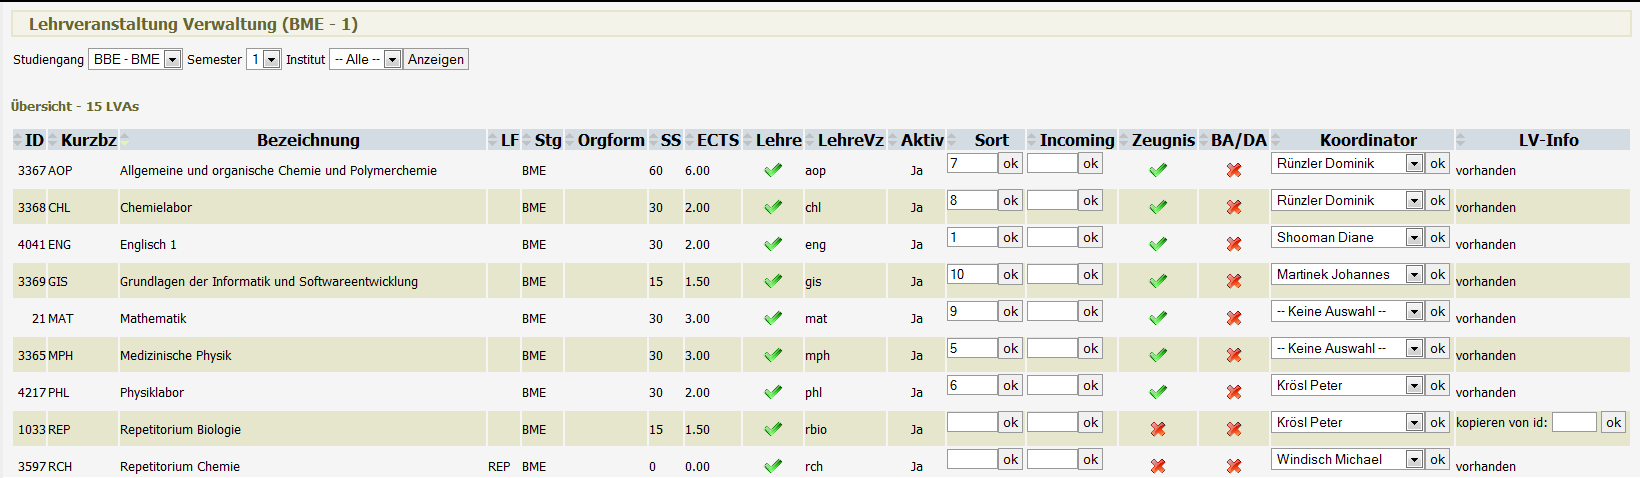
\includegraphics[height=70mm, width=155mm]{FAS_LV1.png}}
			\markier{1}{72}{61}{1}{-1}
			\markier{2}{86}{61}{1}{-1}
			\markier{2}{93}{61}{1}{-1}
			\markier{3}{100}{61}{1}{-1}
			\markier{4}{107}{61}{1}{-1}
			\markier{5}{120}{61}{1}{-1}
			\markier{6}{134}{61}{1}{-1}
		\end{picture}
    \caption{Lehrveranstaltungen}
		\label{LV1}
  \end{center}
\end{figure}

\chapter{Lehreinheiten}
\label{lehreinheiten}
\begin{figure}
	\begin{center}
    \begin{picture}(128,34)
			\put(20,0){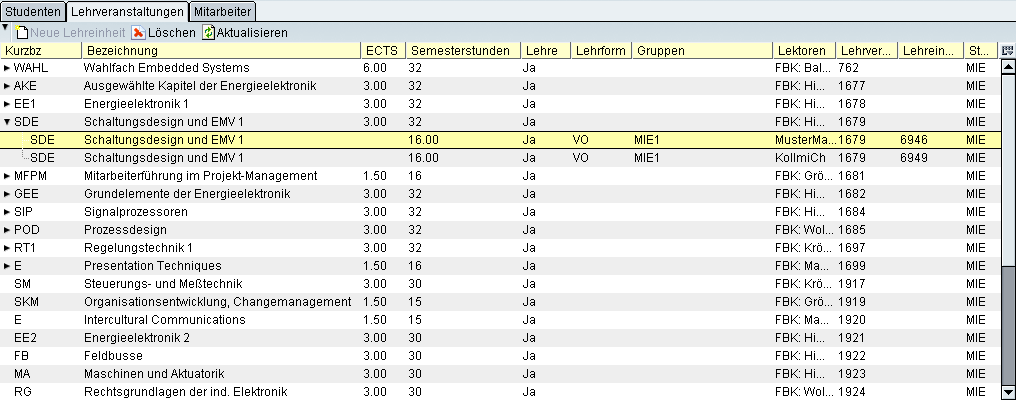
\includegraphics[height=34mm, width=108mm]{FAS_LE1.png}}
			\markier{1}{15}{25}{3}{-1}
			\markier{2}{15}{20}{3}{1}
		\end{picture}
    \caption{Lehrveranstaltungs�bersicht mit Lehreinheiten}
		\label{LE1}
  \end{center}
\end{figure}
Abbildung \ref{LE1} zeigt das Listenfeld mit einer Anzeige von Lehrveranstaltungen und Lehreinheiten. 
\begin{enumerate}
	\item Lehrveranstaltung: Eine Lehrveranstaltung ist ein Teil des Curriculums und scheint auf dem Zeugnissen der Studenten auf. Eine Lehrveranstaltung kann aus mehreren Lehreinheiten, auch unterschiedlicher Art, bestehen.
	\item Lehreinheit: Eine Lehreinheit ist ein Teil des stattfindenden Unterrichts und mu� immer einer Lehrveranstaltung zugeordnet sein. Lehreinheiten werden im Stundenplan verplant und scheinen in den Lehrauftr�gen der Lektoren auf.
\end{enumerate}
Es gibt mehrere M�glichkeiten wie eine Lehrveranstaltung im Unterricht (Lehreinheiten) umgesetzt werden kann:
\begin{itemize}
	\item Eine Gruppe - ein Lektor: Es wird eine Lehreinheit angelegt, zu der die Gruppe und der Lektor zugeordnet werden.
	\item Mehrere Gruppen - ein Lektor: Es mu� f�r jede Gruppe eine Lehreinheit angelegt werden, denen der gleiche Lektor zugeteilt wird. Ausnahme: Findet der Unterricht f�r alle gleichzeitig statt, reicht eine Lehreinheit aus, der der Lektor zugeordnet wird.
	\item Eine Gruppe oder mehrere Gruppen - mehrere Lektoren: Findet der Untericht zusammen zur gleichen Zeit im gleiche Raum statt, wird nur eine Lehreinheit angelegt, ansonsten wird f�r jeden Unterrichtsteil eine Lehreinheit angelegt, der dann die entsprechenden Gruppen und Lektoren zugeteilt werden.
\end{itemize}
\underline{Beispiel:}\\
Abbildung \ref{LE1} zeigt die mit \textit{1} markierte Lehrveranstaltung \textsl{Schaltungsdesign und EMV1} mit 32 Semesterstunden und 3.0 ECTS-Punkten. Diese 32 Stunden sind die Unterrichtsstunden aus der Studentensicht. Darunter, etwas einger�ckt, befinden sich zwei Lehreinheiten zu jeweils 16 Stunden, denen verschiedene Lektoren aber die gleiche Gruppe zugeordnet sind. Die 16 Stunden bei der Lehreinheit sind die Unterrichtsstunden des Lektors und m�ssen daher in Summe nicht zwingend die Semesterstunden der Lehrveranstaltung ergeben.
Hier finden die 32 Stunden des Unterrichts in zwei Teilen zu je 16 Stunden zu unterschiedlichen Zeiten ohne �berschneidung f�r die zugeordnete Gruppe statt.\\

\achtung{\textbf{Wichtig} Findet der Unterricht zeitlich oder r�umlich getrennt statt, mu� der Unterricht in mehrere Lehreinheiten geteilt werden!}\\
\section{Lehreinheit anlegen}
\begin{figure}
	\centering
	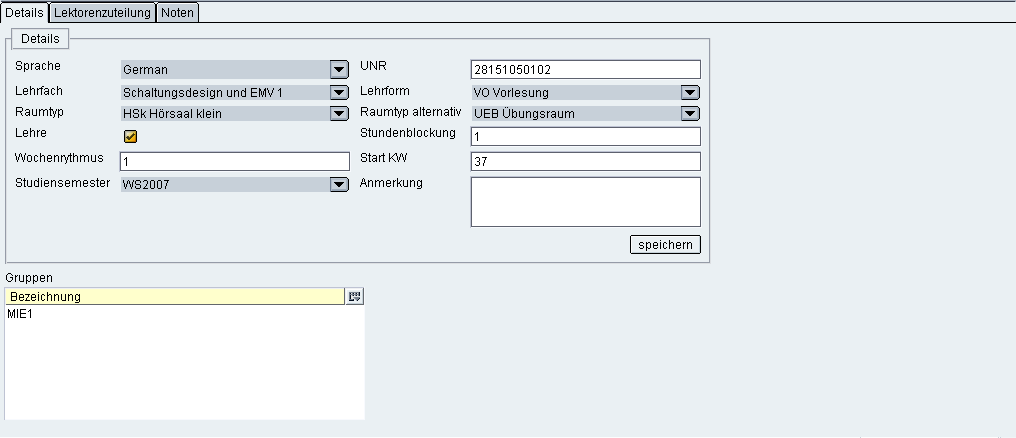
\includegraphics[width=0.75\textwidth]{FAS_LE2.png}
	\caption{LE-Eigenschaften}
	\label{LE2}
\end{figure}
Um eine neue Lehreinheit anzulegen, mu� zuerst der Studiengang im linken Fenster und dann die �bergeordnete Lehrveranstaltung im Karteiblatt Lehrveranstaltungen im oberen Fenster ausgew�hlt werden. Mit einem Klick auf die Taste \textit{Neue Lehreinheit}, die sich oberhalb der LV-/LE-Liste befindet (siehe auch Abbildung \ref{LE1}), wird das Anlegen einer neuen LE vorbereitet und im unteren Fenster, die Anzeige der Attribute eingeblendet. Abbildung \ref{LE2} zeigt das Detailfester mit bereits eingegebenen Werten.
\begin{itemize}
	\item Sprache: In welcher Sprachen wird der Unterricht abgehalten? Zur Auswahl stehen zur Zeit German, English, Espanol.
	\item UNR: Die Unterrichtsnummer wird automatisch nach dem ersten Speichern der Lehreinheit vergeben vergeben. Wenn man bei mehreren Lehreinheiten die gleiche UNR manuell eingibt, werden diese zusammen verplant.
	\item Lehrfach: Das Lehrfach stellt die Verbindung zum Fachbereich dar.
	\item Lehrform: Hier wird die Form des Unterrichts ausgew�hlt, z.B. Seminar, Vorlesung oder �bung.
	\item Raumtyp und Raumtyp alternativ: Diese beiden Felder dienen zur Auswahl des Raumtyps, dessen R�ume �ber die Einrichtung und Gr��e verf�gen, die f�r den Unterricht notwendig sind, bzw. dem Ersatz, wenn alle R�ume des gew�nschten Typs besetzt sind.
	\item Lehre: Wenn angehakt, wird diese Lehreinheit in den Stundenplan einbezogen.
	\item Stundenblockung: Die Stundenblockung gibt an, wie gro� die w�chentliche Unterrichtszeit ist, der in einem St�ck verplant wird.
	\item Wochenrythmus: Der Wochenrythmus gibt an in welchem Intervall (z.B. w�chentlich oder alle 2 Wochen) der Unterricht stattfindet.
	\item Start KW: Die Start-Kalenderwoche gibt die Wochen an, in der der Unterricht beginnt.
	\item Studiensemester: Hier wird ausgew�hlt, in welchem Studiensemester der Unterricht stattfindert (z.B. WS2007).
	\item Anmerkung: Besonderheiten, die bei der Erstellung des Stundenplans ber�cksichtigt werden sollen, k�nnen hier eingegeben werden. 
\end{itemize}
\section{Gruppen zuweisen}
Die Gruppenzuweisung erfolgt per 'Drag And Drop' indem die Gruppe mit der Maus vom linken Bereich in das Listenfeld \textsl{Gruppen} unterhalb der Details der Lehrveranstaltung gezogen wird (Siehe Abbildung \ref{LE4}).
\begin{figure}
	\centering
	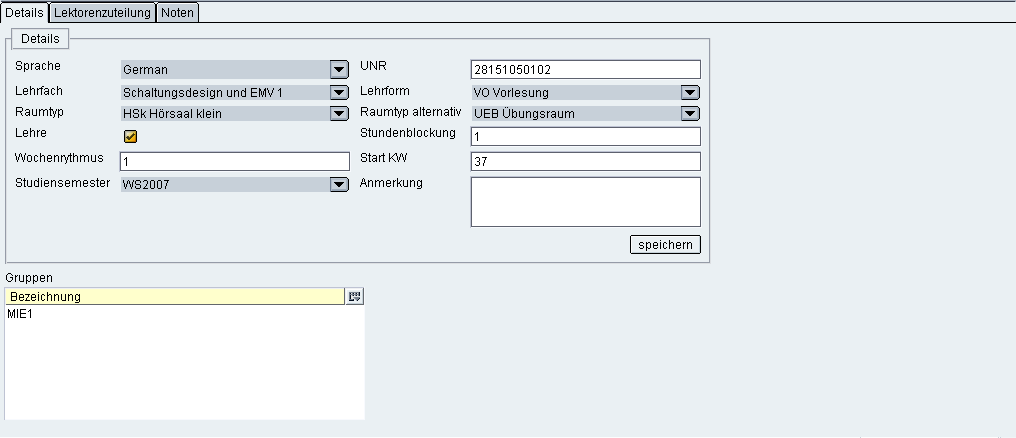
\includegraphics[width=0.75\textwidth]{FAS_LE2.png}
	\caption{Gruppen zuweisen}
	\label{LE4}
\end{figure}
\subsection{Wahlf�cher}
Es wird f�r alle Wahlf�cher je eine zugeh�rige Spezialgruppe angelegt, in die dann die teilnehmenden Studenten hineingezogen werden. Studenten anderer Studieng�nge k�nnen oft nicht direkt zugeordnet werden, da die Zugriffsrechte dies nicht erlauben. Studenten anderer Studieng�nge m�ssen mit der Suchfunktion im Listenfeld 2 gefunden werden und dann von dort in die entsprechende Spezialgruppe in Listenfeld 1 gezogen werden.

\achtung{\textbf{Wichtig} Die studiengangsfremden Studenten m�ssen in Spezialgruppen und auf keinen Fall in Lehrverbandsgruppen (z.B. 1A1, 5B3, etc.) gezogen werden, da es sonst zu Problemen im Herkunftsstudiengang kommt!}\\

\subsection{Incoming}
Incoming-Studenten werden in ihrem Studiengang im Semester 0I angelegt und dort einzeln in Untergruppen (0I1, 0I2,...) aufgeteilt. Die Untergruppe eines Incoming-Studenten wird nun einer Lehreinheit der vom Studenten ausw�hlten Lehrveranstaltung zugeordnet.

\section{Lektoren zuweisen}
Die Zuweisung von Lektoren erfolgt per 'Drag And Drop'. Zuerst im unteren Fenster auf die Kateikarte \textsl{Lektorenzuteilung} wechseln. Danach im linken Fenster auf die Karteikarte \textsl{Lektor} wechseln und die gew�nschte Person mit der Maus in das Listenfeld in der Karteikarte \textsl{Lektorenzuteilung} hineinziehen. Wie in Abbildung \ref{LE3} zu sehen, befindet sich der Name nun in der Liste. Rechts davon sind die Lektorendaten f�r diese Lehreinheit angezeigt bzw. einzugeben.
\begin{itemize}
	\item Lehrfunktion: Hier wird die Funktion der Person innerhalb der Lehreinheit bestimmt. Um einen Lektor im CIS fett gedruckt darzustellen, muss hier LV-Leitung ausgew�hlt werden.
	\item Lektor: Diese Feld zeigt den Namen der gew�hlten Person an.
	\item Semesterstunden: Anzahl der Stunden, die ausgezahlt werden.
	\item Planstunden: Anzahl der Unterrichtsstunden, die im Stundenplan verplant werden.
	\item Stundensatz: Bezahlung pro Unterrichtsstunde.
	\item Faktor: Faktor mit dem der Stundensatz mulipliziert wird. Im Normalfall 1.0, wenn z.B. eine Mehrbelastung durch eine gro�e Studentenzahl besteht, kann mit einer Erh�hung des Faktors das Entgelt f�r diese Lehreinheit erh�ht werden.
	\item Anmerkung: Hier k�nnen zus�tzliche Informationen eingegeben werden.
	\item BIS-Melden: Eingabe, ob dieser Unterricht in der BIS-Meldung ber�cksichtigt wird. 
\end{itemize}
\begin{figure}
	\centering
	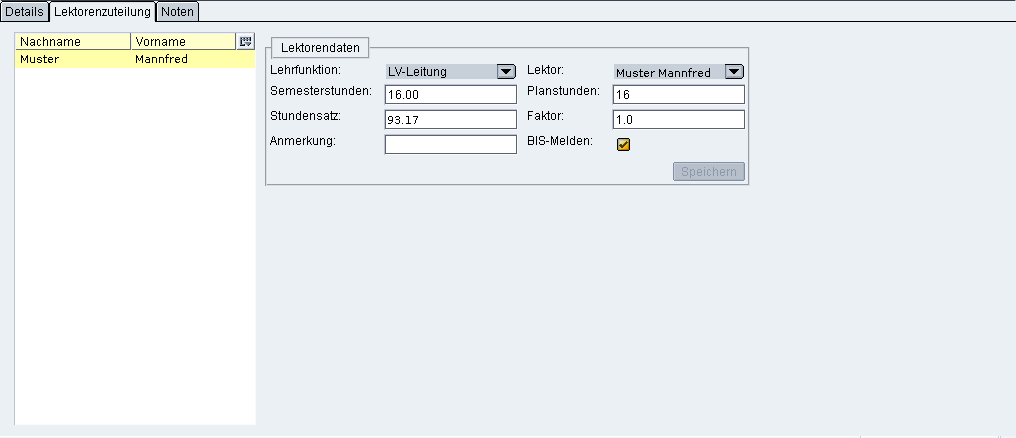
\includegraphics[width=0.75\textwidth]{FAS_LE3.png}
	\caption{Lektoren zuweisen}
	\label{LE3}
\end{figure}

\achtung{
Freie Lektoren d�rfen nicht mehr als 130 Stunden pro Semester unterrichten da diese sonst Fix Angstellt werden m�ssen.. Falls die Zuteilung diese Grenze �berschreiten sollte, wird der Datensatz NICHT gespeichert und eine entsprechende Fehlermeldung erscheint.\\
Bei Fixen Lektoren liegt die Grenze bei 320 Stunden. Hier erscheint jedoch nur eine Warnung. Die Daten werden dennoch gespeichert.
}\\

\chapter{Lehrauftrag}
\label{lehrauftrag}
\info{Definition: Der Lehrauftrag enth�lt die Stunden, die von einem Lektor im Laufe des kommenden Semesters gehalten werden m�ssen (inklusive Betreuungen). Der Lehrauftrag wird den Lektoren vor Beginn des Semesters zur Unterschrift vorgelegt.}\\
\section{Erstellen eines Lehrauftrags}
\underline{Lehrauftrag f�r einen Lektor:}\\Im Tab Lektor Studiengang und Lektor ausw�hlen und rechts auf Lehrauftrag klicken.\\ \\
\underline{Lehrauftrag f�r alle Lektoren eines Studiengangs:}\\Studiengang ausw�hlen und im Men�punkt \textbf{Berichte -  Lehrauftr�ge} klicken.\\ \\
\underline{Lehrauftrag f�r eine Firma erstellen:}\\
Es besteht die M�glichkeit den Lehrauftrag auf den Namen einer Firma auszustellen.\\ \\
Folgende Schritte sind dazu n�tig:
\begin{itemize}
	\item Die Firma unter \textbf{Extras - Firmenverwaltung} anlegen.
	\item Beim Lektor wird unter \textbf{Kontakt} eine neue Adresse angelegt(siehe \ref{kontakte}):
	\begin{itemize}
	 	\item Diese Adresse ist die Firmenadresse, an die der Lehrauftrag gesendet wird.
	 	\item Die Adresse muss als Zustelladresse markiert sein.
	 	\item Im Feld Firma muss die Firma ausgew�hlt werden.
	\end{itemize}
\end{itemize}
\begin{figure}
	\centering
	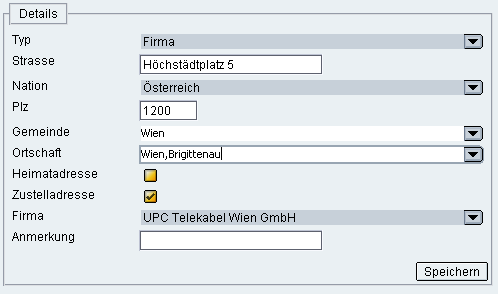
\includegraphics[width=0.75\textwidth]{FAS_Kontakte_Firma.png}
	\caption{Firmenkontakte}
	\label{firmenkontakt}
\end{figure}
\achtung{\textbf{Wichtig} Eine Lehrveranstaltung scheint nur am Lehrauftrag auf, wenn eine Gruppe zugeteilt ist!}\\
\\
Um alle Lehrauftr�ge eines bestimmten Lektors anzuzeigen k�nnen Sie den Lektor ausw�hlen und den Men�punkt Berichte->Lehre->LV-Planung->Excel/HTML w�hlen.

\chapter{Noten}
\label{noten}
\begin{figure}
	\centering
	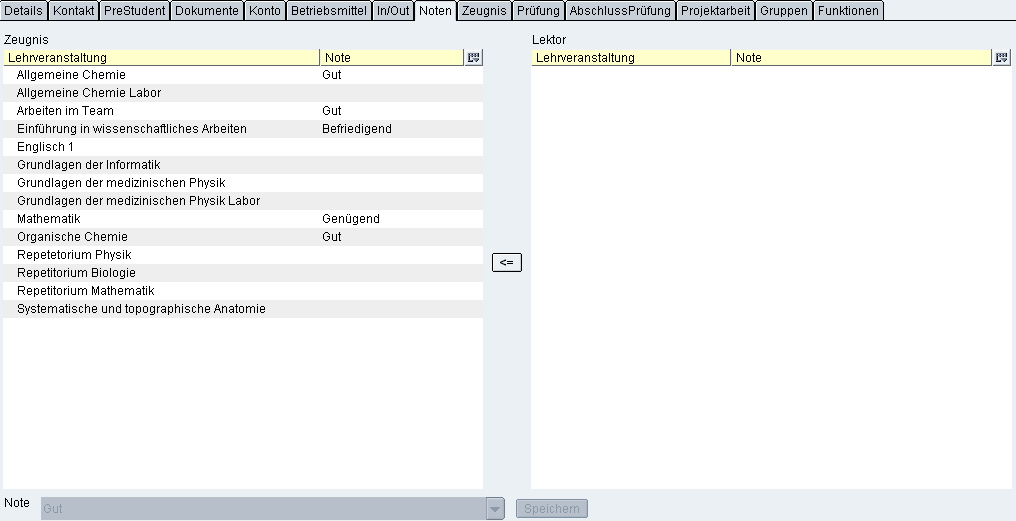
\includegraphics[width=0.75\textwidth]{FAS_Noten1.png}
	\caption{Die Karteikarte Noten}
	\label{noten1}
\end{figure}
\section{Aufbau der Karteikarte}
\begin{itemize}
	\item Listenfeld links: In diesem Fenster befinden sich alle Lehrveranstaltungen, denen der Student indirekt �ber Gruppen zugeordnet ist. Die hier eingetragenen Noten scheinen auf dem Semesterzeugnis auf sofern das die Lehrveranstaltungseinstellugen zulassen.
	\item Listenfeld rechts: Hier werden die aktuellen Noten, die die Lektoren eingegeben haben, angezeigt. Unterscheiden sich Noten von denen der gleichen Lehrveranstaltung im linken Listenfeld, wird die betreffende Zeile vorselektiert.
	\item Button <=: �bertragen von Noten vom Lektoreneintrag in die Liste der Zeugnisnoten.
\end{itemize}
\section{Noteneingabe und -�bergabe}
Einzelne Noten k�nnen in der Karteikarte \textit{Noten} eingetragen werden. Dazu befindet sich am unteren Rand der Karteikarte ein Auswahlfeld in dem die Note der im linken Listenfeld ausgew�hlten Lehrveranstaltung bestimmt werden kann. \\
Noten k�nnen aber auch vom Lektor auf der CIS-Seite eingegeben werden. Die aktuellste Eintragungen scheinen dann in der rechten Liste auf. Unterscheiden sich Noten von bereits �bernommenen, werden sie vorselektiert angezeigt und k�nnen direkt durch Klicken der \textit{<=}-Taste �bernommen werden. Wurde eine Lehrveranstaltung dem Studenten angerechnet, kann diese Eintragung nur manuell ge�ndert werden.\\
Es besteht auch eine M�glichkeit, die Noten einer Lehrveranstaltung zu �bernehmen, ohne jeden Studenten einzeln aufrufen zu m�ssen. Dazu �ffnet man im Listenfeld 2 die entsprechende Lehrveranstaltung und wechselt im Datenfeld dann in die Karteikarte \textit{Noten}. Hier werden in der linken Liste die an der Lehrveranstaltung teilnehmenden Studenten und im rechten Listenfeld die Studenten mit der vom Lektor zuletzt eingetragenen Note aufgelistet. Um die Noten zu �bernehmen, werden die entsprechenden Zeilen in der rechten Liste markiert und mit der \textit{<=}-Taste in die linke Liste kopiert.\\

\info{Wenn die Assistenz eine Note ver�ndert (bspw die Note einer Nachpr�fung eintr�gt) dann wird die Note des Lektors nicht mehr zur �bernahme markiert auch wenn diese dann unterschiedlich zur Zeugnisnote ist. (d.h. wenn das Benotungsdatum der Zeugnisnote j�nger ist als das Benotungsdatum des Lektors)}\\

\chapter{Pr�fungen}
\label{pruefungen}
\begin{figure}
	\centering
	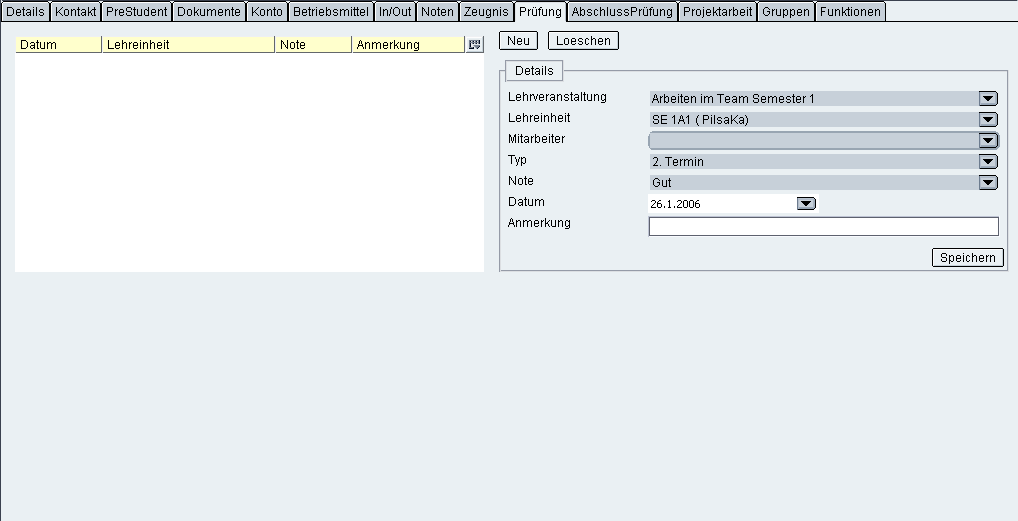
\includegraphics[width=0.75\textwidth]{FAS_Pruefung1.png}
	\caption{Die Karteikarte Pr�fung}
	\label{pruefung1}
\end{figure}
Die Karteikarte \textit{Pr�fung} (siehe Abbildung \ref{pruefung1} besteht aus einem Listenfeld auf der linken Seite und dem Detaildatenbereich auf der rechten Seite und wird f�r die Eintragung von (Wiederholungs-)Pr�fungen verwendet.\\

Wenn eine Pr�fung angelegt wird, wird automatisch die Zeugnisnote aktualisiert.\\
\textbf{Ausnahme:} Wenn das Pr�fungsdatum \underline{vor} dem Benotungsdatum der Zeugnisnote liegt. Hier wird die Pr�fung eingetragen die Zeugnisnote aber nicht ver�ndert. Zus�tzlich erscheint auch eine Warnmeldung, dass die Note nicht ins Zeugnis �bernommen wurde.

\section{Eingabe von Pr�fungen}
Ein Klick auf den Button \textit{Neu} startet den Eingabevorgang. Danach werden die Felder des \textit{Details}-Bereich bef�llt:
\begin{itemize}
	\item Lehrveranstaltung: Die Lehrveranstaltung, in der die Pr�fung erfolgt ist.
	\item Lehreinheit: Hier wird die Lehreinheit ausgew�hlt, die der Student besucht hat.
	\item Mitarbeiter: Der Mitarbeiter, der die Note vergibt.
	\item Typ: Es gibt 3 Pr�fungstypen: den 1.Termin, den 2.Termin (Wiederholung) und die kommissionelle Pr�fung.
	\item Note: Hier kann die Pr�fungsnote ausgew�hlt werden.
	\item Datum: Das Datum der Pr�fung.
	\item Anmerkung: Hier k�nnen zus�tzliche Informationen eingegeben werden.
\end{itemize}
Ein Klick auf den Button \textit{Speichern} beendet mit dem Eintrag der Daten in die Datenbank die Eingabe.

\idee{\textbf{Tipp} Die Pr�fungsnote des Erstantritts mu� im Regelfall nicht eingegeben werden. Bei der Eintragung des Zweitantritts wird der Erstantritt automatisch mit angelegt!}\\

\chapter{Zeugnis}
\label{zeugnis}
Um Zeugnisse zu Erstellen, m�ssen zuerst die Studierenden in der Liste markiert werden. Danach kann das Zeugnis f�r diese Personen �ber den Men�punkt Dokumente->Zeungis erstellt werden.\\
Es wird immer das Zeugnis des aktuell gew�hlten Studiensemesters erzeugt. Das angezeigte Ausbildungssemester wird dem Status entnommen.\\
\\
\subsection{Noten}
Am Zeugnis werden alle Noten angezeigt, die im Karteireiter Noten eingetragen sind, unabh�ngig davon, ob die Person noch tats�chlich zu dieser Lehrveranstaltung zugeteilt ist.\\
\\
Noten von einzelnen Lehrveranstaltungen k�nnen am Zeugnis ausgeblendet werden. Siehe dazu \ref{lehrveranstaltung}\\
\\
Die Reihenfolge der Lehrveranstaltungen am Zeugnis kann �ber die Lehrveranstaltungsverwaltung ge�ndert werden. Siehe dazu \ref{lehrveranstaltung}\\
\\
\subsection{Projektarbeiten}
Projektarbeiten die im Zuge einer Lehrveranstaltung ausgearbeitet werden, k�nnen am Zeugnis angezeigt werden. Dazu muss die Projektarbeit mit der Lehrveranstaltung verkn�pft sein. Siehe dazu \ref{projektarbeit}\\
\subsection{Auslandsaufenthalt}
Bei Studierenden mit Auslandsaufenthalt, muss im Karteireiter In/Out der Bereich Outgoing (Zeugnis) ausgef�llt werden.\\
Wenn dieser Bereich bef�llt ist, scheint am Zeugnis der Auslandsaufenthalt mit einem entsprechenden Infotext auf.
\subsection{Archivierung}
\begin{figure}
	\centering
	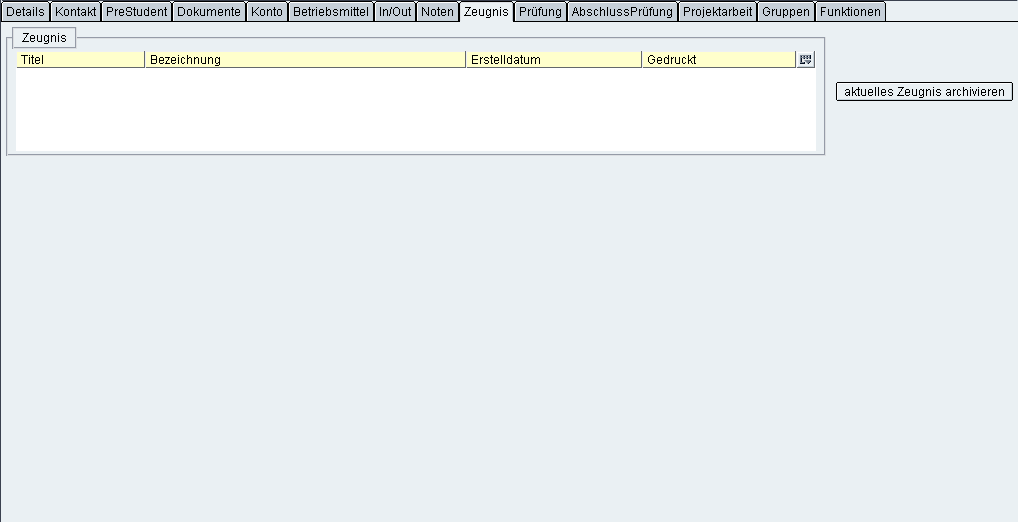
\includegraphics[width=0.75\textwidth]{FAS_Zeugnis1.png}
	\caption{Die Karteikarte Zeugnis}
	\label{zeugnis1}
\end{figure}
Die Karteikarte \textit{Zeugnis}, wie in Abbildung \ref{zeugnis1} gezeigt, hat den Zweck Semesterzeugnisse f�r eine sp�tere Verwendung zu speichern. Dazu wird in das gew�nschte Studiensemester gewechselt und der Student ausgw�hlt. Durch Klicken auf den Button \textit{aktuelles Zeugnis archivieren} wird das Zeugnis des ausgew�hlten Studenten im gew�hlten Studiensemester als Pdf-Datei erzeugt und gespeichtert. Nach Abschlu� des Vorgangs wird das Zeugnis im Listenfeld mit bereits vorhandenen angezeigt. Mit einem Doppelklick wird eine Pdf-Datei ge�ffnet und kann dann gedruckt werden. Ein Rechtsklick bringt die Option das markierte Zeugnis zu l�schen.

Es gibt auch die M�glichkeit die Zeugnisse von mehreren Studenten gleichzeitig zu Archivieren in dem alle Studenten markiert werden und dann auf \textit{aktuelles Zeugnis archivieren} geklickt wird.
\chapter{Freif�cher}
\label{Freif�cher}
Es gibt 2 Verschiedene Arten von Freif�chern\\
- Freif�cher die �ber die FH verrechnet werden\\
- Freif�cher die vom Studiengang verrechnet werden\\
\\

Freif�cher die �ber die FH verrechnet werden, werden im Studiengang 0 (ETW) angelegt. Diese Freif�cher scheinen im CIS unter dem Punkt Freif�cher auf.
Studenten haben die M�glichkeit sich �ber die CIS zu diesen Freif�chern anzumelden. \\
\\
Freif�cher die vom Studiengang verrechnet werden, werden im jeweiligen Studiengang angelegt. F�r diese Freif�cher k�nnen sich die Studenten NICHT �ber die CIS-Seite anmelden.\\
\\

\subsection{Drucken von Best�tigungen}
Im FAS k�nnen Zertifikate f�r den Besuch der Freif�cher ausgedruckt werden. Folgende Schritte sind dazu n�tig: \\
- Freifach im Karteireiter Lehrveranstaltung ausw�hlen\\
- Student im Karteireiter Noten mit der rechten Maustaste anklicken\\
- Freifaecher-Zertifikat erstellen\\
\\
Die angezeigten Lehrinhalte auf dem Freifaecherzertifikat werden Aufgrund der LV-Infos erstellt. Wenn Sie diesen Text �ndern wollen, �ndern Sie im CIS unter LV-Infos das Feld Lehrinhalte.

\achtung{Das Zertifikat kann nur im Karteireiter Lehrveranstaltung gedruckt werden.\\
	Im Karteireiter des Studenten steht diese Option nicht zur Verf�gung}\\

\chapter{Projektarbeit}
\label{projektarbeit}
\section{Die Karteikarte Projektarbeit}
\begin{figure}
	\centering
	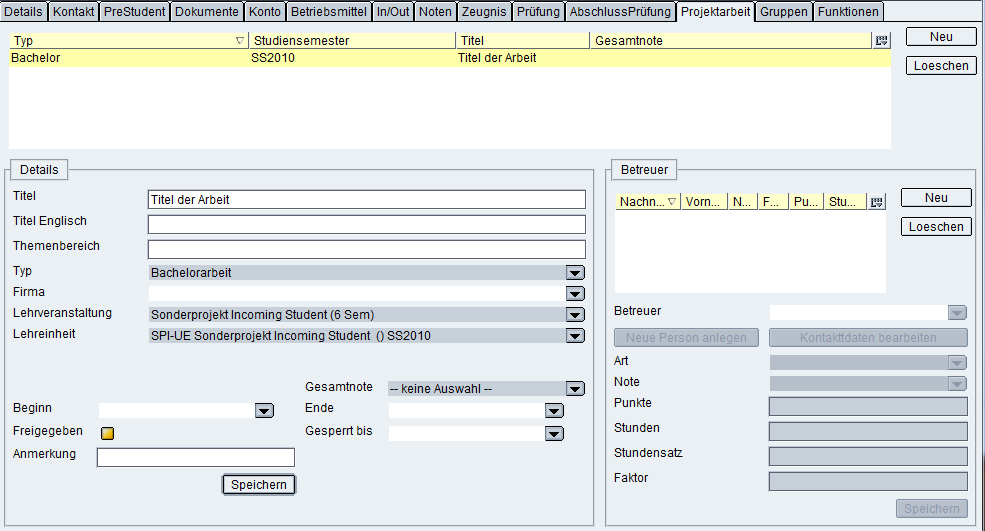
\includegraphics[width=0.75\textwidth]{FAS_Projektarbeit1.png}
	\caption{Karteikarte Projektarbeit}
	\label{Karl}
\end{figure}
Die Karteikarte \textit{Projektarbeit} besteht aus drei Teilen. Im oberen Bereich befindet sich ein Listenfeld mit allen Projektarbeiten des Studenten. Darunter links finden sich im Rahmen \textit{Details} die Daten der Projektarbeit. Rechts k�nnen Betreuer der Projektarbeit angelegt werden.
\subsection{Projektarbeitlistenfeld}
In dem Listenfeld werden alle Projektarbeiten des Studenten angezeigt. \\
Durch Dr�cken der Taste 
\includegraphics{Listenfeld_ConfigButton.png} wird ein kleines Fenster aufgeklappt, in dem  markiert werden kann, welche Spalten im Listenfeld angezeigt werden sollen. Die Taste \textit{Neu} dient zum Anlegen neuer Projektarbeiten, die Taste \textit{Loeschen} zum Entfernen einer Projektarbeit. Zum L�schen mu� zuvor die entsprechende Projektarbeit markiert werden.
\subsection{Details}
Dieser Teil umfa�t mehrere Eingabe- und Auswahlfelder. Der Themenbereich wird mit dem Titel einer Bachelor- oder Diplomarbeit auf dem Zeugnis ausgegeben. \\
Eine Projektarbeit kann neben einer Bachelorarbeit oder einer Diplomarbeit, ein Berufspraktikum, ein Praxissemester oder eine Projektarbeit im engeren Sinn sein. Diese Projektarbeiten scheinen nicht am Zeugnis auf. Soll ein Berufspraktikum oder ein Praxissemester dennoch auf einem Semesterzeugnis aufscheinen, mu� der �bergeordneten Lehreinheit eine oder mehrere Gruppen zugewiesen werden. Die Zeugnisnoten werden den Studenten der Gruppe �ber die Karteikarte \textit{Noten} eingetragen. Die Art der eingetragenen Projektarbeit wird mit dem Auswahlfeld \textit{Typ} bestimmt.\\
Darunter befindet sich ein Auswahlfeld f�r die Firma an der die Projektarbeit durchgef�hrt wurde. \\
Um eine Firma auszuw�hlen muss zuerst ein Teil des Namens der Firma in das Feld eintragen werden. Danach kann aus dem DropDown Men� die entsprechende Firma ausgew�hlt werden.
Mit den Eigabefeldern \textit{Lehrveranstaltung} und \textit{Lehreinheit} wird die Projektarbeit mit der �bergeordneten Lehreinheit verkn�pft. Vor der Auswahl der Lehreinheit ist auf die Einstellung des korrekten Studiensemesters zu achten.\\
In der Folge wird die Gesamtnote, das Beginn- und Endedatum der Projektarbeit angegeben. Das Endedatum wird bei Bachelor- und Diplomarbeiten auch auf dem Pr�fungsprotokoll der Abschlu�pr�fung ausgegeben. Abschlie�end kann eine Sperre der Arbeit eingegeben und eine Anmerkung eingegeben werden.
\subsection{Betreuer}
Das Listenfeld und die beiden Tasten funtionieren analog dem oberen Listenfeld.\\
Zuerst wird der Name des Betreuers ausgew�hlt. Um das Angebot an Betreuern einzugrenzen, sollten drei oder mehr Buchstaben des Nachnamens eingegeben und danach die Pfeiltaste der Auswahlbox gedr�ckt werden. Dann kann der passende Betreuer aus einer Liste mit �bereinstimmungen ausgesucht werden.\\
In Folge werden die Art des Betreuers, die vom Betreuer vergebene Note und der Zeitaufwand ausgew�hlt. Die Liste der Betreuertypen umfa�t Betreuer und Begutachter von Diplomarbeiten. Wenn der Betreuer und der notengebende Begutachter ein und diesselbe Person sind, kann die Eingabe des Betreuer entfallen und sowohl Stunden wie auch Beurteilung beim Begutachter eingetragen werden.\newpage
\section{Anlegen einer Diplomarbeit}
\label{Kapitel_Anlegen_DA}
\begin{figure}
	\centering
	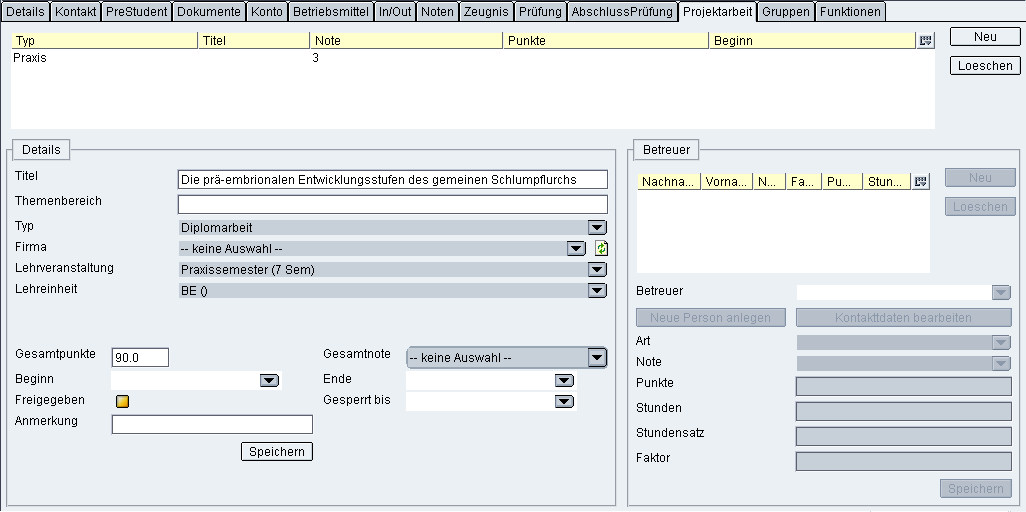
\includegraphics[width=0.75\textwidth]{FAS_DA1.png}
	\caption{Anlegen einer Diplomarbeit 1}
	\label{DA1}
\end{figure}
Zum Eintragen einer neuen Projektarbeit sind zuallererst das Studiensemester und der Student auszuw�hlen. Durch Dr�cken der Taste \textit{Neu} werden die Eingabefelder freigegeben und k�nnen wie in Abbildung \ref{DA1} gezeigt mit den Daten der Projektarbeit bef�llt werden. Nach der Eingabe des Titels und optional des Themenbereichs der Projektarbeit wird der Typ der Projektarbeit ausgew�hlt. Als n�chstes erfolgt die Zuordnung der Projektarbeit zu einer Lehreinheit. Dazu wird im Auswahlfeld \textit{Lehrveranstaltung} eine Lehrveranstaltung und im Auswahlfeld darunter die dazugeh�rige Lehreinheit markiert, der die Diplomarbeit zugeordnet werden soll.

\achtung{\textbf{Wichtig} bei der Auswahl der Lehreinheit ist, da� das \textbf{richtige Studiensemester gew�hlt} wurde, da ansonsten die Projektarbeit auf keinem Semesterzeugnis und auf dem Lehrauftrag des falschen Semesters aufscheint.}

\begin{figure}
	\centering
	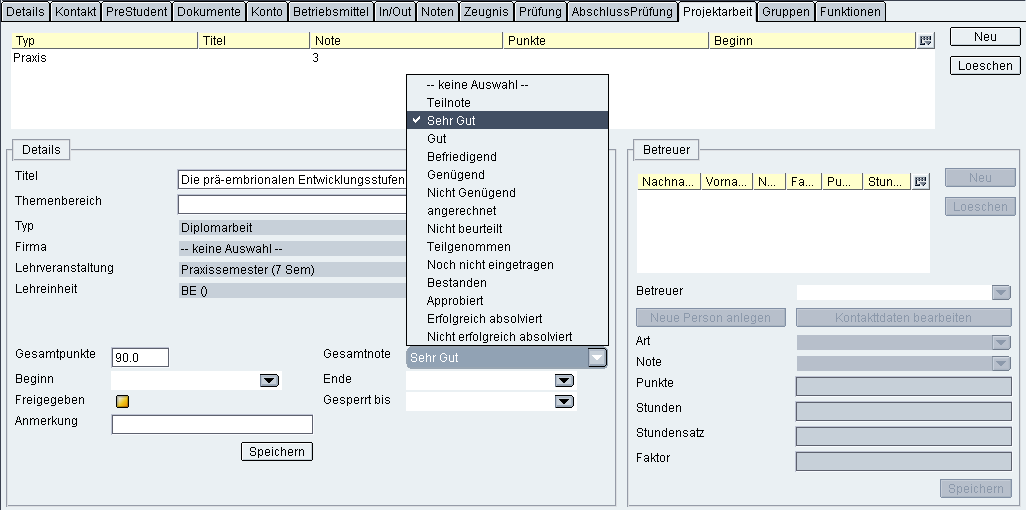
\includegraphics[width=0.75\textwidth]{FAS_DA2.png}
	\caption{Anlegen einer Diplomarbeit 2}
	\label{DA2}
\end{figure}
\newpage
Abbildung \ref{DA2} zeigt wie nach der Eingabe der Gesamtpunkte die Note ausgew�hlt werden kann.\\
\begin{figure}
	\centering
	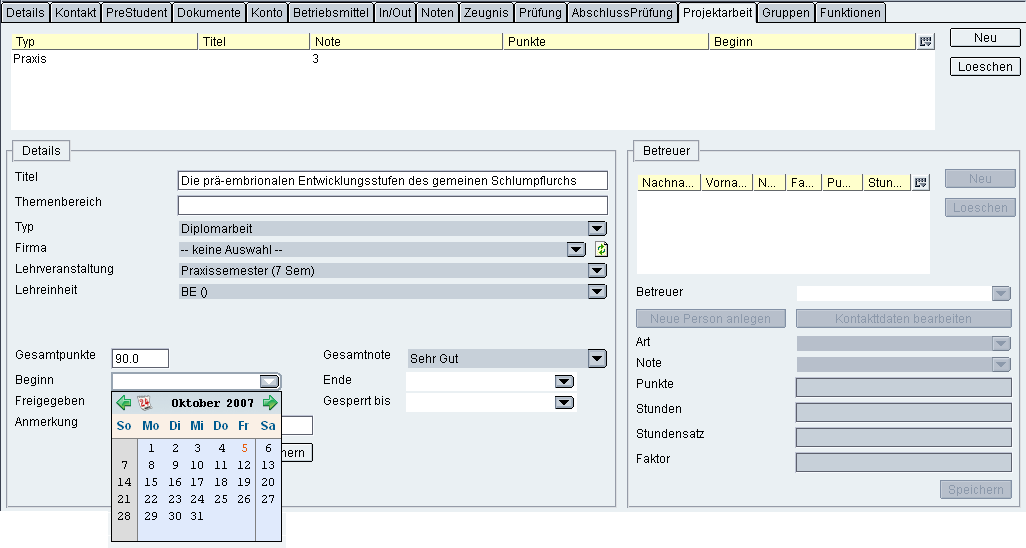
\includegraphics[width=0.75\textwidth]{FAS_DA3.png}
	\caption{Anlegen einer Diplomarbeit 3}
	\label{DA3}
\end{figure}
Bei den Feldern \textit{Beginn}, \textit{Ende} und \textit{Gesperrt bis} kann das Datum in das Feld eingegeben werden oder wie in Abbilung \ref{DA3} in einem Kalenderblatt ausgew�hlt werden. Durch Klicken auf die beiden gr�nen Pfeile kann das angezeigte Monat gewechselt werden.\\
\begin{figure}
	\centering
	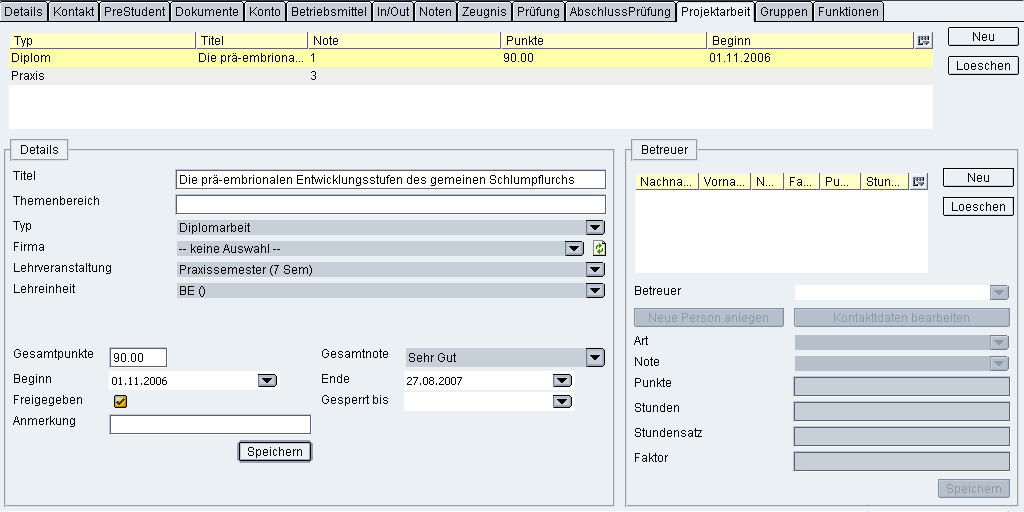
\includegraphics[width=0.75\textwidth]{FAS_DA4.png}
	\caption{Anlegen einer Diplomarbeit 4}
	\label{DA4}
\end{figure}
Ein Klick auf die Taste \textit{Speichern} schie�t den Vorgang ab und die Projektarbeit scheint danach, wie in Abbildung \ref{DA4} zu sehen, markiert im Listenfeld auf.
\section{Anlegen einer Bachelorarbeit}
Die Eingabe einer Bachelorarbeit erfolgt analog zu der einer Diplomarbeit -- siehe Kapitel \ref{Kapitel_Anlegen_DA} auf Seite \pageref{Kapitel_Anlegen_DA}. Beim Auswahlfeld \textit{Typ} ist Bachelorarbeit auszuw�hlen.
\section{Anlegen eines Praktikums}
Berufspraktika sind f�r FH-Bachelor- und FH-Diplomstudieng�nge verpflichtend vorgeschrieben. Es ist dabei sicherzustellen, dass das Berufspraktikum den Ausbildungszielen des FH-Studiengangs entspricht und dass die Studierenden ihrem Qualifikationsniveau entsprechend eingesetzt werden.
Der Fachhochschulrat hat beschlossen, dass die Integration von Berufspraktika in FH-Masterstudieng�ngen nur unter den bestimmten Voraussetzungen (siehe Homepage FHR) zul�ssig ist.
(http://www.fhr.ac.at)
\begin{figure}
	\centering
	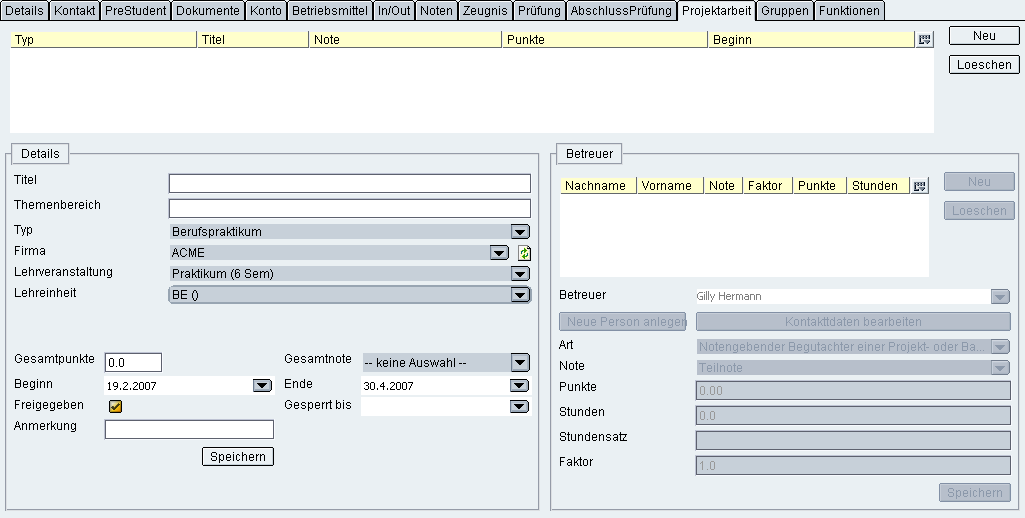
\includegraphics[width=0.75\textwidth]{FAS_Praktikum1.png}
	\caption{Anlegen eines Praktikums 1}
	\label{Praktikum1}
\end{figure}
Bei der Eingabe eines Berufspraktium kann im Textfeld \textit{Titel} der Titel einer abschlie�enden Projektarbeit festgehalten werden, der Inhalt dieses Feldes wird zur Zeit aber auf keinem Dokument ausgegeben. Danach wird die Firma ausgew�hlt, bei der das Praktikum durchgef�hrt wird. \\
Sollte die gew�nschte Firma nicht in der Auswahlliste vorhanden sein, kann sie �ber den Men�punkt \textsc{Extras/Firmenverwaltung} des Hauptmen�s angelegt werden. Danach mu� die Taste 
\includegraphics{icon_aktualisieren.png} angeklickt werden, damit die Auswahlliste aktualisiert wird.\\
Nach der Eingabe des Beginn- und Endedatums wird das Anlegen des Praktikums durch Klicken der Taste \textit{Speichern} abgeschlossen. Das Berufspraktikum erscheint danach wie in Abbildung \ref{Praktikum2} markiert in der Liste auf.
\begin{figure}
	\centering
	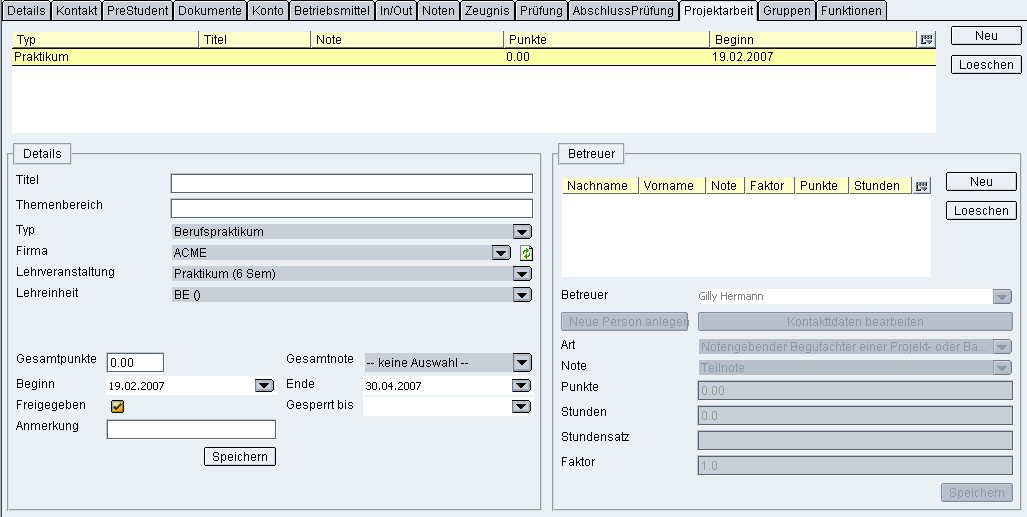
\includegraphics[width=0.75\textwidth]{FAS_Praktikum2.png}
	\caption{Anlegen eines Praktikums 2}
	\label{Praktikum2}
\end{figure}
\section{Anlegen eines Betreuers}
Soll einer Projektarbeit ein Betreuer hinzugef�gt werden, mu� zuallererst die betreffende Projektarbeit im Listenfenster markiert werden. Danach wird der Eingabevorgang durch Klicken der Taste \textsl{Neu} im \textit{Betreuer}-Bereich rechts unten begonnen (Siehe Abbildung \ref{Betreuer1}. Danach werden die Daten des Betreuers eingegeben. Zur Auswahl des Namens sollten, wie in Abbildung \ref{Betreuer2} gezeigt, zumindest 3 Buchstaben des Nachnamen in das Feld eingegeben und danach die Pfeiltaste rechts neben dem Feld angeklickt werden. Dann kann der gew�nschte Betreuer ausgew�hlt werden. Nachfolgend werden noch folgende Daten eingegeben:
\begin{itemize}
	\item Art: Hier wird die Art der Betreuung passend zu der Art der Projektarbeit bestimmt (Siehe Abbildung \ref{Betreuer3}. 
	\item Note: Beurteilung der Arbeit mittels Notenraster.
	\item Punkte: Beurteilung der Arbeit mittels Punktetabelle.
	\item Stunden: Arbeitsaufwand in Stunden des Betreuers. Dieser Wert scheint auf dem Lehrauftrag auf.
	\item Stundensatz: Betrag, den der Betreuer pro Stunde bekommt. Dieser Wert scheint auf dem Lehrauftrag auf.
	\item Faktor: Betrag mit dem der Stundensatz multipliziert wird. Dieser Wert scheint auf dem Lehrauftrag auf.
\end{itemize}
Durch Anklicken der Taste \textit{Speichern} wird der Vorgang abgeschlossen und der Betreuer in die Datenbank �bertragen (Siehe Abbildung \ref{Betreuer4}).

\achtung{\textbf{Wichtig} Die Eintragungen \textit{Stunden}, \textit{Stundensatz} und \textit{Faktor} werden f�r den Lehrauftrag des Lektors ben�tigt! Der Bruttobetrag am Lehrauftrag errechnet sich aus Stunden*Stundensatz*Faktor.}

\begin{figure}
	\centering
	\includegraphics[width=0.75\textwidth]{FAS_DA_Betreuer1.png}
	\caption{Anlegen eines Betreuers 1}
	\label{Betreuer1}
\end{figure}
\begin{figure}
	\centering
	\includegraphics[width=0.75\textwidth]{FAS_DA_Betreuer2.png}
	\caption{Anlegen eines Betreuers 2}
	\label{Betreuer2}
\end{figure}
\begin{figure}
	\centering
	\includegraphics[width=0.75\textwidth]{FAS_DA_Betreuer3.png}
	\caption{Anlegen eines Betreuers 3}
	\label{Betreuer3}
\end{figure}
\begin{figure}
	\centering
	\includegraphics[width=0.75\textwidth]{FAS_DA_Betreuer4.png}
	\caption{Anlegen eines Betreuers 4}
	\label{Betreuer4}
\end{figure}
\newpage
\section{Verwendung der Daten}
Hier eine Auflistung der einzelnen Datenfelder und wof�r Sie verwendet werden.
\begin{figure}[!htbp]
    \begin{center}
        \begin{picture}(140,80)
            \put(0,0){\includegraphics[width=140mm]{FASo_Projektarbeit_Diplomarbeit.png}}
            \markier{1}{20}{62}{1}{-2}
            \markier{2}{20}{53}{1}{-1}
						\markier{3}{20}{40}{1}{0}
        \end{picture}
        \caption{Datenfelder bei Projektarbeit}
        \label{FASo_Projektarbeit_Diplomarbeit}
    \end{center}
\end{figure}

\begin{itemize}
	\item Titel (siehe Abbildung \ref{FASo_Projektarbeit_Diplomarbeit} Pkt. 1)
	Erscheint auf: Zeugnis
	\item Themenbereich (siehe Abbildung \ref{FASo_Projektarbeit_Diplomarbeit} Pkt. 2)
	\item Firmenauswahl: Die Firma ist nur bei Berufspraktika anzugeben. Wenn eine Firma eingetragen wird, erscheint am Zeugnis hinter der LV der Zustatz \textit{bei Firma xyz}
\end{itemize}
%Siehe Seite \pageref{Karl} Abbildung \ref{Karl}

\chapter{Bachelor- und Diplompr�fungen}
\label{abschlusspruefungen}
Diplom- und Bachelorpr�fungen sind, da beide den Abschlu� eines Studiums darstellen, in der Karteikarte Abschlu�pr�fung einzugeben. Da es Unterschiede im Aufbau der Pr�fungen gibt, werden diese nachfolgend getrennt erkl�rt.
\section{Diplompr�fung}
Die abschlie�enden Pr�fungen der Master- und Diplomstudieng�nge werden als Diplompr�fungen bezeichnet. Sie bestehen aus:
\begin{enumerate}
	\item Diplomarbeit
	\item Kommissioneller Pr�fung:
	\begin{itemize}
		\item Pr�sentation der Diplomarbeit (Eingabe siehe Kapitel \ref{Kapitel_Anlegen_DA})
		\item Pr�fungteil technisches Fach
		\item Pr�fungsteil nichttechnisches Fach
	\end{itemize}
\end{enumerate}
Die Abbildung \ref{DAPruefung} zeigt den Aufbau der Eingabemaske f�r Diplompr�fungen bestehend aus folgenden Feldern:\\
links:
\begin{itemize}
	\item Typ: Hier ist \textsl{Diplompr�fung} auszuw�hlen.
	\item Vorsitz: Zur Auswahl des Namens sollten zumindest 3 Buchstaben des Nachnamen in das Feld eingegeben und danach die Pfeiltaste rechts neben dem Feld angeklickt werden. Dann kann die gew�nschte Person ausgew�hlt werden.
	\item Abschlu�beurteilung: Hier wird die Gesamtbeurteilung aus \textsl{mit ausgezeichnetem Erfolg bestanden}, \textsl{mit gutem Erfolg bestanden}, \textsl{bestanden} und \textsl{nicht bestanden} ausgew�hlt.
	\item Akademischer Grad: Auswahl des akademischen Grads, der nach bestandener Pr�fung verliehen wird. 
	\item Datum: Datum der Pr�fung.
	\item Sponsion: Datum der Sponsion.
\end{itemize}
rechts:
\begin{itemize}
	\item Pruefer 1 (Diplomarbeit): Die Auswahl des Pr�fers erfolgt analog zu der des Vorsitzes.
	\item Pruefer 2: Die Auswahl des Pr�fers erfolgt analog zu der des Vorsitzes.
	\item Anmerkung: Hier k�nnen zus�tzliche Informationen eingegeben werden.
\end{itemize}
Durch Anklicken der Taste \textit{Speichern} wird der Vorgang abgeschlossen und die Daten werden in die Datenbank �bertragen.
\begin{figure}
	\centering
	\includegraphics[width=0.75\textwidth]{FAS_Abschlusspruefung1.png}
	\caption{Diplompr�fung eintragen}
	\label{DAPruefung}
\end{figure}
\section{Bachelorpr�fung}
Die abschlie�enden Pr�fungen der Bachelorstudieng�nge werden als Bachelorpr�fungen bezeichnet. Sie sind  kommissionelle Pr�fungen bestehend aus bis zu drei Teilpr�fungen.
Die Abbildung \ref{BAPruefung} zeigt den Aufbau der Eingabemaske f�r Bachelorpr�fungen bestehend aus folgenden Feldern:\\
links:
\begin{itemize}
	\item Typ: Hier ist \textsl{Bachelorpr�fung} auszuw�hlen.
	\item Vorsitz: Zur Auswahl des Namens sollten zumindest 3 Buchstaben des Nachnamen in das Feld eingegeben und danach die Pfeiltaste rechts neben dem Feld angeklickt werden. Dann kann die gew�nschte Person ausgew�hlt werden.
	\item Abschlu�beurteilung: Hier wird die Gesamtbeurteilung aus \textsl{mit ausgezeichnetem Erfolg bestanden}, \textsl{mit gutem Erfolg bestanden}, \textsl{bestanden} und \textsl{nicht bestanden} ausgew�hlt.
	\item Akademischer Grad: Auswahl des akademischen Grads, der nach bestandener Pr�fung verliehen wird. 
	\item Datum: Datum der Pr�fung.
	\item Sponsion: Datum der Abschlu�feier. Wenn keine stattfindet, dann sollte hier ebenfalls das Datum der Pr�fung eingegeben werden.
\end{itemize}
rechts:
\begin{itemize}
	\item Pruefer 1 - 3 : Die Auswahl der Pr�fer erfolgt analog zu der des Vorsitzes.
	\item Anmerkung: Hier k�nnen zus�tzliche Informationen eingegeben werden.
\end{itemize}
Durch Anklicken der Taste \textit{Speichern} wird der Vorgang abgeschlossen und die Daten werden in die Datenbank �bertragen.
\begin{figure}
	\centering
	\includegraphics[width=0.75\textwidth]{FAS_Abschlusspruefung2.png}
	\caption{Bachelorpr�fung eintragen}
	\label{BAPruefung}
\end{figure}
\section{Rechtsklick-Funktionen}
Mit einen Rechtsklick auf einen Abschlu�pr�fungsdatensatz lassen sich vier Dokumente ausdrucken. 
\begin{itemize}
	\item Pruefungsprotokoll: Dieses Dokument wird \underline{vor} dem Pr�fungstermin ausgedruckt. Die Pr�fungskommission f�llt das Protokoll w�hrend der Pr�fung aus. Die Reihenfolge der Bachelor-/Diplomarbeiten die am Protokoll aufscheinen h�ngt vom Beginndatum der Arbeit ab. Falls mehr als 2 Arbeiten vorhanden sind, werden die mit dem j�ngsten Beginndatum angezeigt.
	\item Pruefungszeugnis: Das Pr�fungszeugnis wird nach der Abschlu�pr�fung ausgedruckt und dem Studenten mit seinen Abschlu�unterlagen ubergeben.
	\item Urkunde: Die Urkunde best�tigt als formelles Dokument den Studienabschlu�.
	\item Urkunde englisch 
\end{itemize}
\chapter{Betriebsmittel}
\label{betriebsmittel}
Als Betriebsmittel werden hier auszuleihende Gegenst�nde wie Zutrittskarten oder Schl�ssel verstanden.
\section{Aufbau der Karteikarte Betriebsmittel}
Die Abbildung \ref{Betriebsmittel1} zeigt den Aufbau der Karteikarte \textsl{Betriebsmittel}:
\begin{itemize}
	\item Listenfeld: Hier werden alle Betriebsmittel, die der Student ausgeliehen hat angezeigt.
	\item Details-Bereich: Im Details-bereich k�nnen die Betriebsmitteldaten eingegeben und ver�ndert werden.
	\begin{itemize}
		\item Typ: Welcher Gegenstand wurde entliehen. Auswahl z.Z.: Schl�ssel, Zutrittskarte, Laptop.
		\item Nummer: Schl�sselnummer bzw Kartennummer
		\item Nummer 2: Feld f�r die zweite Kartennummer (zb bei Dualtranspondern)
		\item Inventarnummer: Feld zur Auswahl der Inventarnummer
		\item Beschreibung: Zus�tzliche Informationen zum Betriebsmittel.
		\item Kaution: Einbezahlte Kaution.
		\item Anmerkung: Zus�tzliche Informationen zur Entleihung.
		\item Ausgegeben am: Datum der Ausgabe.
		\item Retour am: Datum der R�ckgabe.
	\end{itemize}
	\item Button \textsl{Neu}: Start der Eingabe einer Betriebsmittelentlehnung.
	\item Button \textsl{Loeschen}: L�schen eines markierten, fehlerhaften Eintrags.
	\item Button \textsl{�bernahmebest�tigung}: Hier wird eine �bernahmebest�tigung f�r das gew�hlte Betriebsmittel erstellt
\end{itemize}
\begin{figure}
	\centering
	\includegraphics[width=0.75\textwidth]{FAS_Betriebsmittel1.png}
	\caption{Die Karteikarte Betriebsmittel}
	\label{Betriebsmittel1}
\end{figure}
\section{Eingabe von Betriebsmittelentlehnungen}
\underline{Beispiel}:\\
Student XY erh�lt einen Laptop vom Studiengang f�r seine Projektarbeit.
Nach der Auswahl des Studenten wird die Karteikarte \textsl{Betriebsmittel} ge�ffnet und mit der Taste \textit{Neu} der Eingabevorgang begonnen. Zuerst wird bei Typ \textsl{Inventar} ausgew�hlt. Nun wird statt den Nummern-Feldern ein Inventarnummer Feld angezeigt. Hier wird die Inventarnummer des Laptops eingetragen (zB 88+02+0005). Hier kann auch nur ein Teil der Inventarnummer eingetragen werden, die gefundenen Vorschl�ge werden nach dem Eintippen im Dropdown angezeigt. Zuletzt wird noch das aktuelle Datum als Entlehndatum eingegeben. Abgeschlossen wird der Eingabevorgang durch Klicken der Taste \textsl{Speichern}.\\
Damit das Inventar hier gefunden wird, muss dieses zuerst inventarisiert werden. Dies geschieht im Vilesci unter \textsl{Inventar}\\
\underline{Beispiel}:\\
Student XY erh�lt zum Studienbeginn die Zutrittskarte mit der Nummer 408627633833. \\
Nach der Auswahl des Studenten wird die Karteikarte \textsl{Betriebsmittel} ge�ffnet und mit der Taste \textit{Neu} der Eingabevorgang begonnen. Zuerst wird bei Typ \textsl{Zutrittskarte} ausgew�hlt, dann darunter die Nummer 408627633833 der Zutrittskarte in das linke Feld eingegeben. Im Feld \textsl{Beschreibung} k�nnte jetzt noch eine genauere Beschreibung der Zutrittskarte eingegeben werden. Dann wird der Betrag der Kaution eingegeben. Zuletzt wird noch das aktuelle Datum als Entlehndatum eingegeben. Abgeschlossen wird der Eingabevorgang durch Klicken der Taste \textsl{Speichern}.\\
\underline{Beispiel}:\\
Student XY hat sein Studium beendet und will seine Zutrittskarte zur�ckgeben.\\
Nach der Auswahl des Studenten wird der Karteikarte \textsl{Betriebsmittel} ge�ffnet und die Eintragung mit der Nummer der Zutrittskarte im Listenfeld markiert. Jetzt kann das R�ckgabedatum in das Feld \textsl{Retour am} eingetragen werden. Durch Klicken der Taste \textsl{Speichern} wird der Datensatz aktualisiert und das R�ckgabedatum gespeichert.\\
\underline{Beispiel}:\\
Student YZ ist seine Zutrittskarte leider abhanden gekommen.\\
In diesem Fall wird im \textsl{Anmerkung}-Feld vermerkt, da� der Student YZ am heutigen Tag den Verlust der Karte gemeldet hat und das \textsl{Retour am}-Feld auf das aktuelle Datum gesetzt.
\chapter{Dokumente}
\label{dokumente}
Ein Student mu� zu Beginn seines Studiums verschiedenen Dokumente in Original vorzeigen und Kopien abgeben. In dieser Karteikarte wird festgehalten, welche bereits vorgelegt wurden.
Abbildung \ref{Dokumente1} zeigt den Aufbau der Karteikarte \textsl{Dokumente}:
\begin{itemize}
	\item Liste \textsl{Noch nicht abgegeben}: In diesem Listenfeld werden alle m�glichen und noch nicht abgegebenen Dokumente aufgelistet.
	\item Liste \textsl{Abgegeben}: Auslistung aller abgegebenen Dokumente.
	\item Button \textsl{=>}: Die im linken Feld markierten Dokumente-Eintr�ge werden in die rechte Liste der abgegebenen Dokumente �bertragen.
	\item Button \textsl{<=}: Dieser Korrekturbutton verschiebt markierte Dokumente-Eintr�ge in die Liste der noch nicht abgegebenen Dokumente.
	\item Button \textsl{Filter}: Wird dieser Button gedr�ckt, werden in der Studentenliste oberhalb des Krateireiters \textsl{Dokumente} alle jene Studenten angezeigt, die Dokumente noch nicht abgegeben haben.
\end{itemize}
\begin{figure}
	\centering
	\includegraphics[width=0.75\textwidth]{FAS_Dokumente1.png}
	\caption{Die Karteikarte Dokumente}
	\label{Dokumente1}
\end{figure}
\chapter{Funktionen}
\label{funktionen}
Abbildung \ref{Funktionen1} zeigt den Aufbau der Karteikarte \textsl{Funktionen}:
\begin{itemize}
	\item Listenfeld: Zeigt die Funktionen der Person an. 
	\item Details: 	Im Details-bereich k�nnen die Funktionen-Daten eingegeben und ver�ndert werden.
	\begin{itemize}
		\item Funktion: Funktion, die die Person aus�bt.	
		\item Organisationseinheit: Organisationseinheit in dem die Funktion g�ltig ist.
		\item Institut: In einigen Situationen ist es n�tig, dass sowohl ein Studiengang (Organisationseinheit) und ein Institut zugeordnet werden muss. 
		\item Semester: Semester in dem die Funktion g�ltig ist.
		\item Bezeichnung: Standardm�ssig wird die Bezeichnung von der Funktion �bernommen
		\item G�ltig von: Datum ab dem die Funktion g�ltig ist.
		\item G�ltig bis: Datum bis wann die Funktion g�ltig ist.
	\end{itemize}
	\item Button \textsl{Neu}: Start der Eingabe einer Funktion.
	\item Button \textsl{Loeschen}: L�schen eines markierten Eintrags.
\end{itemize}
\begin{figure}
	\centering
	\includegraphics[width=0.75\textwidth]{FAS_Funktionen1.png}
	\caption{Die Karteikarte Funktionen}
	\label{Funktionen1}
\end{figure}
\section{Anlegen von Funktionen}
\underline{Institutsleiter eintragen:}\\
Folgende Eingaben sind vorzunehmen:
\begin{itemize}
	\item Funktion = Leitung
	\item Organisationseinheit =  Institut/Bereich, der geleitet wird.
\end{itemize}
Abschlie�end \textbf{Speichern} klicken.\\
\underline{Institutskoordinator eintragen:}\\
Es gibt 2 M�glichkeiten Koordinatoren zuzuweisen. 
\begin{itemize}
	\item 1.�ber die Lehrveranstaltung:
	\begin{itemize}
		\item F�r spezielle Lehrveranstaltungen kann ein eigener Koordinator angegeben werden. Diese werden immer Vorrangig angezeigt. Wenn zu einer LV kein Koordinator zugeteilt ist, wird jener Koordinator angezeigt der die Zuteilung �ber die Funktion hat. N�here Information unter \ref{lehrveranstaltung} (Lehrveranstaltung).
	\end{itemize}
	\item 2.�ber die Funktionen
	\begin{itemize}
		\item Funktion = Koordinator
		\item Organisationseinheit = Studiengang der Koordinatorfunktion
		\item Institut = Institut der Koordination
	\end{itemize}
\end{itemize}
\underline{OE-Zuordnung eintragen:}\\
Die Zuordnung zur Organisationseinheit wird ben�tigt um die Hierarchie der Mitarbeiter darzustellen. (Um zB die Freigaben des Urlaubes auf der CIS-Seite verwalten zu k�nnen). Wenn keine OE-Zuordnung eingetragen ist, dann werden beim Eintragen von Urlauben auf der CIS keine Freigabemails versendet.
Folgende Eingaben sind vozunemen:
\begin{itemize}
	\item Funktion = OE-Zuordnung
	\item Organisationseinheit = Organisationseinheit, der die Person zugeordnet werden soll
\end{itemize}

\chapter{BIS-Meldung}
Das BIS-System vereint die Studierenden-, Personal- und F\&E-Datenmeldungen, die aufgrund der Bildungsdokumentationsverordnung-Fachhochschulen des BMBWK sowie der BIS-Verordnung des FHR f�r die unterschiedlichen Adressaten (BMBWK, FHR, Statistik Austria, u.a.) zu erfassen sind. Dies erm�glicht die inhaltliche �berschaubarkeit, gew�hrleistet vor allem aber die erforderliche technische Integration des von unterschiedlicher Seite artikulierten Datenbedarfes in einem einheitlichen Meldesystem.
(BIS Schnittstelle Version 5.1, FHR)
\section{Die Studentenmeldung}
Die BIS-Meldung erfolgt zwei mal im Jahr, im November sind die Studenten- und Personaldaten zu melden und im April die Studenten- und F\&E-Daten. Stichtag f�r die Studentenmeldung ist jeweils der 15. des betreffenden Monats. Der Meldungszeitraum f�r die Personalmeldung ist das vergangene Studienjahr, bei der F\&E-Meldung das vergangene Kalenderjahr. 
\subsection{Plausibilit�tspr�fung}
\begin{figure}
	\centering
	\includegraphics[width=0.75\textwidth]{FAS_BIS_Studenten1.png}
	\caption{Aufruf des Studenten-Plausichecks}
	\label{Plausi}
\end{figure}
FASonline bietet die M�glichkeit, die zu meldenden Daten schon ab Semesterbeginn und nicht erst ab Beginn des Meldemonats zu �berpr�fen. Dazu wird die Plausibilit�tspr�fung, wie in Abbildung \ref{Plausi} gezeigt, aufgerufen. Hier werden die Daten �berpr�ft und fehlende und fehlerhafte Eingaben angezeigt.
\subsection{Erzeugen der XML-Datei}
\label{Erzeugen der XML-Datei}
Die BIS-Meldung teilt sich in zwei Teile. Der erste Teil ist die Testphase und endet am 15. des Meldemonats. Die erstellten XML-Dateien k�nnen in dieser Zeit zur Probe auf die FHR-Seite hochgeladen werden. Am Morgen des 15. sind alle Stati der Studieng�nge wieder auf unbearbeitet zur�ckgesetzt und m�ssen zumindest noch einmal hochgeladen werden. Die zweite Phase beginnt mit dem 15., dem Stichtag, und endet am 30. des Meldemonats.\\
Abbildung \ref{BIS1} zeigt, wie die Erstellung der XML-Datei gestartet wird. Dazu wird der gew�nschte Studiengang im linken Fenster markiert und im Men� unter \textsl{BIS/Studenten} \textit{Meldung generieren} angeklickt.
\begin{figure}
	\centering
	\includegraphics[width=0.75\textwidth]{FAS_BIS_Studenten2.png}
	\caption{Erstellen der XML-Datei1}
	\label{BIS1}
\end{figure}
Nach einigen Plausibilit�ts�berpr�fungen werden ev. Fehler und eine Statistik der Ergebnisse, etwa wie in Abbildung \ref{BIS2},  angezeigt. Die Tabelle zeigt den Inhalt der Meldung in tabellarischer Form an. Die erste Zeile gibt die Semester von 1 bis 8 bei allen Studieng�ngen an, auch wenn diese weniger Semester umfassen, sowie 50 und 60. Die letzten beiden Semesterzahlen stehen f�r Personen, die die Abschlu�pr�fung nicht in der regul�ren Studienzeit gemacht, sondern 1 Jahr bzw. mehrere Jahre �berzogen haben. Die darauffolgenden Zeilen zeigen die aktiven Studenten, Unterbrecher, Abbrecher, Absolventen und Incoming/Outgoing (I/O) in den jeweiligen Semestern an. Die letzte Zeile beinhalten die Anzahl der Bewerber. Das sind alle Studenten, die seit der letzten BIS-Meldung einen Bewerberstatus erhalten und ein H�kchen bei \textit{Zum Reihungstest angetreten} in der Karteikarte \textsl{PreStudent} haben. Ganz rechts in der letzten Zeile scheint die Anzahl der gefundenen Fehler auf rotem Hintergrund auf. 

\achtung{\textbf{Wichtig} Die Personen, bei denen Fehler aufgetreten sind, werden nicht in die XML-Datei geschrieben und somit auch \emph{\textbf{nicht gemeldet}}!}\\\\
\begin{figure}
	\centering
	\includegraphics[width=0.75\textwidth]{FAS_BIS_Studenten3.png}
	\caption{Studenten�bersicht}
	\label{BIS2}
\end{figure}
Unter der Tabelle befindet sich ein Link zur erzeugten XML-Datei. Diese mu� mittels Rechtsklick und \textsl{Link-Ziel speichern} oder in der englischen Seamonkey-Version \textsl{Save Link Target As} auf dem eigenen Computer gespeichert werden, von wo die Datei im n�chsten Schritt auf die FHR-Seite hochgeladen wird.
\subsection{Die FHR-Seite}
\info{Die FHR-Seite (www.fhr.ac.at) ist f�r den Internet Explorer� optimiert und sollte daher nur mit diesem aufgerufen werden. Verwendet man einen anderen Browser, werden manche Funktionalit�ten, wie Mitteilungsfenster, nicht angezeigt.}\\\\
Abbildung \ref{FHR1} zeigt die Startseite der Homepage vom Fachhochschulrat. Zum Einloggen mu� der Login-Button unten in der Mitte angeklickt werden. Danach erscheint eine Eingabeaufforderung  (Abbildung \ref{FHR2} f�r die Eingabe von Benutzername und Passwort. Auf der n�chsten Seite wird mit einem Klick auf den Link \textsl{Applikation starten}, in Abbildung \ref{FHR3} markiert, fortgesetzt. Es erscheint eine Liste aller Studieng�nge f�r die der eingeloggte Anwender Berechtigungen hat (Siehe Abbildung \ref{FHR4}. Mit einem Klick auf die Taste \textsl{Upload}, rechts oben auf der Seite, gelangt man in den Bereich der FHR-Seite, wo die BIS-Meldedatei hochgeladen werden kann.\\
\begin{figure}
	\begin{center}
    \begin{picture}(108,90)
			\put(0,0){\includegraphics[height=90mm, width=108mm]{FAS_FHR1.png}}
			\markier{!}{55}{35}{1}{-1}
		\end{picture}
    \caption{Die FHR-Seite}
		\label{FHR1}
  \end{center}
\end{figure}
\begin{figure}
	\centering
	\includegraphics[width=0.75\textwidth]{FAS_FHR2.png}
	\caption{Login auf der FHR-Seite}
	\label{FHR2}
\end{figure}
\begin{figure}
	\begin{center}
    \begin{picture}(108,90)
			\put(0,0){\includegraphics[height=90mm, width=108mm]{FAS_FHR3.png}}
			\markier{!}{56}{52}{-1}{1}
		\end{picture}
    \caption{Applikation starten}
		\label{FHR3}
  \end{center}
\end{figure}
\begin{figure}
	\begin{center}
    \begin{picture}(108,90)
			\put(0,0){\includegraphics[height=90mm, width=108mm]{FAS_FHR4.png}}
			\markier{!}{90}{60}{1}{1}
		\end{picture}
    \caption{Upload}
		\label{FHR4}
  \end{center}
\end{figure}
\begin{figure}
	\begin{center}
    \begin{picture}(108,90)
			\put(0,0){\includegraphics[height=90mm, width=108mm]{FAS_FHR5.png}}
			\markier{1}{47}{73}{1}{-1}
			\markier{2}{90}{73}{-1}{-1}
			\markier{3}{65}{57}{1}{1}
			\markier{4}{82}{57}{0}{1}
			\markier{5}{88}{57}{0}{1}
		\end{picture}
    \caption{Upload der XML-Datei}
		\label{FHR5}
  \end{center}
\end{figure}
Abbildung \ref{FHR5} zeigt das Upload-Dialogfenster der BIS-Meldung. Zuerst mu� angegeben werden, welche Datei hochgeladen werden soll. Dazu klickt man auf die mit 1 markierte Taste \textsl{Durchsuchen...} und w�hlt im Dialogfenster die Datei des gew�nschten Studiengangs aus. (Anmerkung: Am Ende des Kapitels \ref{Erzeugen der XML-Datei} wurde diese Datei am lokalen PC gespeichert.) Wurde die Datei ausgew�hlt, erscheinen Pfad und Dateiname im Textfester links von der Taste \textsl{Durchsuchen...}. Ein Klick auf die mit 2 markierte Taste \textsl{Upload und Validierung} startet die Daten�bertragung. Nach Beendigunge der �bertragung erscheint ein Hinweisfenster mit Mitteilung, da� der Upload erfolgreich war oder da� bei der �berpr�fung Fehler gefunden wurden. Wurden Fehler gefunden, erscheint im rechten, kleineren Fenster der Name der Datei, die die Auflistung der Fehler beinhaltet. Diese Liste kann nun entweder im linken, gro�en Fenster angesehen werden oder heruntergeladen werden. In beiden F�llen mu� die Datei mit einem Klick auf den Namen markiert werden. Danach wird entweder die mit 3 markierte Taste f�r die Anzeige im Fenster oder die mit 4 markierte Taste f�r den Download angeklickt. Mit der f�nften Taste kann die Fehlerdatei entfernt werden. Nach der Fehlerkorrektur wird diese Prozedur wiederholt, bis der erfolgreiche Upload angezeigt wird. 
\subsection{Fehlerkorrektur}
\begin{figure}
	\begin{center}
    \begin{picture}(108,90)
			\put(0,0){\includegraphics[height=90mm, width=108mm]{FAS_FHR6.png}}
			\markier{1}{82}{57}{0}{1}
			\markier{2}{65}{59}{1}{1}
		\end{picture}
    \caption{Fehlermeldung nach Upload}
		\label{FHR6}
  \end{center}
\end{figure}
Wenn beim Upload Fehler auftreten, werden diese in einer Datei gespeichert, deren Name im rechten Fenster angezeigt wird. Um die Fehlermeldungen anzuzeigen, wird der Dateiname (1) und dann \textsl{Inhalt anzeigen} (2) angeklickt. Dann erscheinen im linken Fenster, wie im Bild \ref{FHR6} gezeigt, die Fehlermeldungen. \\
Zur Fehlerkorrektur kann die PersKz des Studenten (im Bild \ref{FHR6} in den Zeilen 9 und 11) aus der Meldung kopiert und mittels der Suchfunktion der Student im FAS angezeigt werden.
\newpage
\section{Die Mitarbeitermeldung}
Bei der November-BIS-Meldung werden neben den Studentendaten auch die Mitarbeiterdaten gemeldet.
\subsection{Plausibilit�tspr�fung}
\begin{itemize}
	\item checkVerwendung:
	Pr�ft die vorhanden Verwendungen auf Plausibilit�t. Hier werden keine Daten ver�ndert oder gel�scht sondern nur Warnungen ausgegeben.
	\item checkFunktion:
	Generiert aufgrund der Lehrauftr�ge die BIS-Funktionen. (bis.tbl\_bisfunktion)\\ Wenn bereits Eintr�ge vorhanden sind, werden diese aktualisiert, ansonsten neu angelegt. Die Funktionseintr�ge zu denen es keinen Lehrauftrag gibt werden angezeigt aber NICHT automatisch gel�scht. Es wird aber der SQL Befehl angezeigt mit dem diese Funktionen dann gel�scht werden k�nnen.
	\item Import:
	Hier kann man die Verwendungen und Funktionen anhand der vorj�hrigen BIS-Meldung importieren. Dazu wird die Mitarbeiter-Meldung des Vorjahres hochgeladen:
		\begin{itemize}
		\item Funktionen werden ins System importiert (...wenn eine passende Verwendung gefunden wurde oder bei dieser Person keine andere Verwendung existiert. Wenn eine Verwendung gefunden wurde, diese aber nicht mit derjenigen aus der BIS-Meldung �bereinstimmt, werden die zugeh�rigen Funktionen nicht angelegt)
		
		\item Verwendungen werden nur ins System importiert wenn KEINE Verwendung f�r die Person vorhanden ist.
		\end{itemize}
	Es werden nur Verwendungen/Funktionen importiert. Die anderen BIS-Daten werden hier nicht ber�cksichtigt.
\end{itemize}
\subsection{Erzeugen der XML-Datei}
Im Men�punkt \textsl{BIS} befindet sich unter \textsl{Mitarbeiter} mit textsl{Meldung generieren} der Aufruf zur Erzeugung der xml-Datei f�r die BIS-Personalmeldung. Als Ergebnis zeigt dann folgende Daten an:
\begin{itemize}
	\item Gesamtanzahl der Mitarbeiter
	\item Anzahl der Mitarbeiter mit echtem Dienstvertrag
	\item Anzahl der Mitarbeiter mit freiem Dienstvertrag
	\item Eine Auflistung von Dateninkonstistenzen unter der �berschrift \textsl{Nicht plausieble BIS-Daten (f�r Meldung XXXX)}
	\item Ein Link zur xml-Datei f�r die Personalmeldung. Diese Datei mit der rechten Maustaste anklicken und mit \textsl{Link-Ziel speichern unter} lokal abspeichern. Diese Datei wird dann auf der FHR-Seite wie ein Studiengang der Studentenmeldung hochgeladen.
\end{itemize}
\section{Die F\&E - Projektmeldung}
\subsection{Plausibilit�tspr�fung}
\subsection{Erzeugen der XML-Datei}
\subsection{Die FHR-Seite}
\chapter{Mitarbeiter}
\label{mitarbeiter}
\begin{figure}
	\centering
	\includegraphics[width=0.75\textwidth]{FAS_Mitarbeiter2.png}
	\caption{Ansicht Mitarbeiterbereich}
	\label{Mitarbeiter2}
\end{figure}
\section{Anzeigefilter}
\begin{itemize}
	\item Alle: Es werden im Listenfeld 2 alle Mitarbeiter ohne Einschr�nkungen angezeigt.
	\item FixAngestellte: Es werden alle Mitarbeiter angezeigt, bei denen \textit{Fixangestellt} (in der Karteikarte \textit{Stammdaten} der Mitarbeiter rechts unten) angehakt ist. 
	\item FreiAngestellte: Es werden alle Mitarbeiter angezeigt, bei denen \textit{Fixangestellt} (in der Karteikarte \textit{Stammdaten} der Mitarbeiter rechts unten) nicht angehakt ist.
	\item Aktive: Die nachfolgenden Filter listen nur Mitarbeiter auf, die als aktiv (in der Karteikarte \textit{Stammdaten} der Mitarbeiter rechts oben) gekennzeichnet sind.
	\begin{itemize}
		\item FixAngestellte: wie FixAngestellte unter \textit{Alle}, aber hier nur aktive Mitarbeiter.
		\item FreiAngestellte: wie FreiAngestellte unter \textit{Alle}, aber hier nur aktive Mitarbeiter.
		\item Karenziert: Es werden hier aktive Mitarbeiter aufgelistet, bei denen eine aktuelle Verwendung (unter Karteikarte \textit{BIS-Daten}) mit Ausmass \textsl{Karenz} eingegeben ist.
		\item Ohne Verwendung: Es werden alle aktiven Mitarbeiter aufgelistet, bei denen keine aktuelle Verwendung eingetragen ist.
		\item Studiengangsleiter: Es werden alle aktiven Mitarbeiter, bei denen zumindest eine Funktion \textit{Leitung} f�r einen Studiengang in der Karteikarte \textit{Funktionen} eingetragen ist.
		\item Institutsleiter: Es werden alle aktiven Mitarbeiter, bei denen zumindest eine Funktion \textit{Leitung} f�r ein Institut in der Karteikarte \textit{Funktionen} eingetragen ist.
	\end{itemize}
	\item Inaktive: Es werden im Listenfeld 2 alle Mitarbeiter angezeigt, die nicht als aktiv (in der Karteikarte \textit{Stammdaten} der Mitarbeiter rechts oben) gekennzeichnet sind. 
	\begin{itemize}
		\item Mit Verwendung: Hier werden Mitarbeiter aufgelistet, die nicht als aktiv gekennzeichnet sind, aber dennoch eine aktuelle Verwendung besitzen.
	\end{itemize}
\end{itemize}
\section{Mitarbeiterdatenkarten}
\subsection{Stammdaten}
Die Karteikarte \textit{Stammdaten} beinhaltet die Personen- und Mitarbeiterdaten des in Listenfeld 2 ausgew�hlten  Mitarbeiters. Besonders zu beachten sind die vier Checkboxen auf dieser Seite:
\begin{itemize}
	\item Aktiv: Diese Checkbox entscheidet ob der Mitarbeiter als aktiv gef�hrt wird. Eine Woche nach der Entfernung des H�kchens wird der Mitarbeiter �ber die Deaktivierung seines Accounts informiert. Der Account wird dann ein Jahr sp�ter nach einem weiteren Benachrichtigungsmail gel�scht.
	\item Lektor: Diese Checkbox mu� markiert sein, damit der Mitarbeiter einer Lehreinheit als Unterrichtender zugewiesen werden kann.
	\item Fixangestellt: Diese Checkbox unterscheidet Mitarbeiter mit einem fixen Arbeitsvertrag von Mitarbeitern mit einem freien Dienstverh�ltnis und wirkt sich auf die Mailverteiler und die Filter der Mitarbeiterverwaltung aus.
	\item Bismelden: Ist diese Checkbox markiert, wird der Mitarbeiter in die BIS-Meldung einbezogen.
\end{itemize}
\subsection{Kontaktdaten}
Die Karteikarte \textit{Kontaktdaten} beinhaltet die Adresse, die E-Mailadresse, Telefon- und Faxverbindungen sowie die Bankverbindungen des Mitarbeiters. Diese Karteikarte entspricht in Aufbau und Funktion der Karteikarte \textit{Kontakt} der Studenten (siehe Kapitel \ref{kontakte}).
\subsection{BIS-Daten}
\begin{figure}
	\centering
	\includegraphics[width=0.75\textwidth]{FAS_BISDaten1.png}
	\caption{BIS-Daten}
	\label{BISDaten1}
\end{figure}
Abbildung \ref{BISDaten1} zeigt die Karteikarte \textit{BIS-Daten}, mit der die BIS-Daten der Mitarbeiter bearbeitet werden. Die Karteikarte besteht aus drei Teilen:
\begin{enumerate}
	\item Verwendung: Die Verwendung des Mitarbeiters ist eine Abbildung des Dienstvertrages.\\
	Der \textit{Verwendung}-Bereich ist ein Listenfeld, das die vergangenen und gegenw�rtigen Verwendungen des Mitarbeiters anzeigt. Mit der Taste \textit{Neu} �ffnet sich ein Eingabefenster mit leeren Eingabefenstern zum Anlegen einer neuen Verwendung. Wird eine Verwendung markiert, kann mit einem Klick auf den Button \textit{Bearbeiten} diese Verwendung ver�ndert werden oder mit einem Klick auf den Button \textit{Loeschen} entfernt werden. \\
	Das Eingabeformular besteht aus folgenden Eingabe- und Auswahlfeldern:
	\begin{itemize}
		\item Beschaeftigungsart 1: Art des Dienstvertrags. In den meisten F�llen \textsl{Echter Dienstvertrag} oder \textsl{Freier Dienstvertrag}
		\item Beschaeftigungsart 2: Auswahl, ob der Dienstvertrag unbefristet oder befristet ist.
		\item Beschaeftigungsausmass: F�r jede einer Person zugewiesenen Kategorie der Besch�ftigungsart 1 (Vertragstypen) ist das entsprechende Besch�ftigungsausma� anhand folgender Einteilung anzugeben.\\
		Das Besch�ftigungsausma� ist definiert als die auf den Berichtszeitraum (12 Monate) umgerechnete Wochenarbeitszeit je Besch�ftigungsverh�ltnis einer Person.
		\begin{table*}
			\centering
				\begin{tabular}{|c|c|}
					\hline
					BeschAusmassCode&BeschAusmassBez\\
					\hline
					1&Vollzeit\\
					\hline
					2&<=15 Wochenstunden\\
					\hline
					3&16-25 Wochenstunden\\
					\hline
					4&26-35 Wochenstunden\\
					\hline
					5&Karenz\\
					\hline
				\end{tabular}
			\caption{BIS - Beschaeftigungsausmass}
			\label{tab:BIS - Beschaeftigungsausmass}
		\end{table*}
		(BIS Schnittstelle Version 5.1, 20.10.2006, FHR)
		\item Verwendung: Mitarbeiter m�ssen einer Verwendungsgruppe zugeordnet werden. Siehe Tabelle \ref{tab:BIS - Verwendung}
		\begin{table*}
			\centering
				\begin{tabular}{|c|c|}
					\hline
					Verwendungscode&VerwendungBez\\
					\hline
					1&Lehr- und Forschungspersonal\\
					&(Academic staff)\\
					\hline
					2&Lehr- und Forschungshilfspersonal\\
					&(Teaching and Research assistants)\\
					\hline
					3&Akademische Dienste f�r Studierende\\
					&(Academic Support)\\
					\hline
					4&Soziale Dienste und Gesundheitsdienste\\
					&(Health and Social Support)\\
					\hline
					5&Studiengangsleiter/in\\
					\hline
					6&Leiter/in FH-Kollegium\\
					\hline
					7&Management\\
					&(School Level Management))\\
					\hline
					8&Verwaltung\\
					&(School Level Administrative Personnel)\\
					\hline
					9&Hauspersonal, Geb�ude-/Haustechnik\\
					&(Maintenance and Operations Personnel)\\
					\hline
				\end{tabular}
			\caption{BIS - Verwendung}
			\label{tab:BIS - Verwendung}
		\end{table*}
		\item Hauptberuflich Lehrende(r): Anzugeben ist, ob es sich um eine/n hauptberuflich Lehrende/n handelt.\\
		Die Angabe \"haupts�chlich Lehrende/r - ja\" ist nur bei den Verwendungscodes 1 (Lehr- und Forschungspersonal), 5 (Studiengangsleiter/in) und 6 (Leiter/in FH-Kollegium) m�glich. F�r die Definition des/der hauptberuflich Lehrenden sind folgende Kriterien relevant: das zeitliche Ausma� der T�tigkeit, der Anteil an den Eink�nften und die Art der T�tigkeit (Profil). (BIS Schnittstelle Version 5.1, 20.10.2006, FHR)
		\item Hauptberuf: Bei nebenberuflich Lehrenden ist die deren Hauptberuf anzugeben und einer Hauptberufkategorie zuzuordnen.
		\item Habilitation
		\item Beginn: Beginndatum der Verwendung.
		\item Ende: Endedatum der Verwendung.
		\item Vertragsstunden: Vertraglich vereinbarte Arbeitsstunden. Dieser Wert wird nicht direkt in der BIS-Meldung verwendet.
	\end{itemize}
	\item Funktion:\\
	In diesem Bereich werden Lehrfunktionen des ausgew�hlten Mitarbeiters festgehalten. Die Eingabe startet mit einem Klick auf den Button \textit{Neu}, dann k�nnen der Studiengang ausgew�hlt und die Semesterwochenstunden (SWS) eingegeben werden.\\
	Mit dem Button \textit{Loeschen} k�nnen markierte Eintr�ge von Funktionen gel�scht werden.
	\item Entwicklungsteam: \\
	In diesem Bereich wird angegeben, ob der Mitarbeiter im Entwicklungsteam von Studieng�ngen war und welche Qualifikation daf�r ausschlaggebend war.
\end{enumerate}
\subsection{Betriebsmittel}
Hier werden die entliehenen Betriebsmittel wie z.B. Schl�ssel festgehalten (siehe Kap. \ref{betriebsmittel}).
\subsection{Funktionen}
In dieser Karteikarte werden die Funktionen der Mitarbeiter, und in welchem Studiengang und Institut diese ausge�bt werden, festgehalten. 
Der Aufbau dieser Karteikarte wird in Kapitel \ref{funktionen} beschrieben.
\section{Neuen Mitarbeiter anlegen}
\begin{figure}
	\centering
	\includegraphics[width=0.75\textwidth]{FAS_Mitarbeiter1.png}
	\caption{Neuen Mitarbeiter anlegen}
	\label{Mitarbeiter1}
\end{figure}
Um einen neuen Mitarbeiter anzulegen, mu� entweder im Listenfeld 1 oder im Listenfeld 2 auf den Karteireiter \textit{Mitarbeiter} geklickt und danach in der Men�leiste des Listenfeld 2 der Button \textit{Neu} angeklickt werden. Dadurch �ffnet sich die in Abbildung \ref{Mitarbeiter1} gezeigte Eingabemaske. Nach der Eingabe der Mitarbeiterdaten und einem klick auf 'Vorschlag laden' wird gepr�ft, ob diese Person bereits im System vorhanden ist. Wenn die gew�nschte Person in der Liste aufscheint, klicken Sie auf den kleinen Kreis neben der Person. Andernfalls w�hlen Sie den Punkt 'Neue Person anlegen' aus. Der Mitarbeiter wird danach mittels \textit{Speichern}-Taste in die Datenbank �bertragen.


\chapter{Men�leisten}
\section{Hauptmen�leiste}
\begin{figure}
	\centering
	\includegraphics[width=0.75\textwidth]{FAS_Menueleiste1.png}
	\caption{Die Hauptmen�leiste}
	\label{menue1}
\end{figure}
\begin{itemize}
	\item Datei: 
  \begin{itemize}
  	\item Beenden: Schlie�t FASonline.
  \end{itemize}	
  \item Bearbeiten: 
	\begin{itemize}
		\item UNDO: Unter diesem Men�punkt werden L�schvorg�nge aufgelistet, die r�ckg�ngig gemacht werden k�nnen.
	\end{itemize}
	\begin{figure}
		\centering
		\includegraphics[width=0.75\textwidth]{FAS_Menueleiste11.png}
		\caption{Die Hauptmen�leiste - Einstellungen}
		\label{menue11}
	\end{figure}
	\item Einstellungen (Abbildung \ref{menue11}): 
	\begin{itemize}
		\item Studiensemester: Auflistung der im Programm angelegten Studienssemester. Das aktuell ausgew�hlte Studiensemester wird im Men� markiert und au�erdem in der Statusleiste (Siehe Abbildung \ref{Grundlagen1} Markierung 4) angezeigt.
		\item Buchungen auf Studiengang filtern: Wenn dieser Men�eintrag markiert wird, scheinen in der Karteikarte \textsl{Konto} nur mehr Buchungen des Studiengangs auf. Ist der Men�eintrag nicht markiert, werden auch Buchungen von anderen Studieng�ngen (z.B. zuvor absolvierter Bachelorstudiengang) angezeigt.
	\end{itemize}
	\begin{figure}
		\centering
		\includegraphics[width=0.75\textwidth]{FAS_Menueleiste12.png}
		\caption{Die Hauptmen�leiste - Berichte}
		\label{menue12}
	\end{figure}
	\item Berichte (Abbildung \ref{menue12}): 
	\begin{itemize}
		\item Lehre
			\begin{itemize}
			\item LV-Planung: Zeigt eine Auflistung der Lehrveranstaltungen eines Studienganges und deren Kosten
			\item Projektarbeit: Hier werden die Projektarbeiten aufgelistet, die dem \textbf{ausgew�hlten Studiensemester} zugeordnet wurden.
			\item Abschlusspr�fung: Es werden hier nur die \textbf{benoteten} Abschlu�pr�fungen, die dem \textbf{ausgew�hlten Studiensemesters} zugeordnet wurden.
			\end{itemize}  
		\item Mitarbeiter
			\begin{itemize}
			\item Koordinatorstunden: Zeigt an, wieviele Stunden die Koordinatoren eines Fachbereichs in den verschiedenen Studieng�ngen unterrichten
			\item Lehrauftragsliste: Erstellt ein Excel Dokument mit den Kosten eines Studienganges Aufgeschl�ssel auf die einzelnen Lektoren
			\end{itemize}  
		\item Student: 
			\begin{itemize}
			\item Fehlende Dokumente: Zeigt eine Liste aller Studenten eines Studienganges/Semesters und die Dokumente die abgegeben wurden.
			\item Personendetails Excel: Erstellt einen Excel-Export der markierten Studenten mit einer Vielzahl an Daten.
			\item �H-Beitr�ge: Erstellt die Liste der zu Zahlenden �H-Beitr�ge
			\item Notenspiegel: Erstellt einen Notenspiegel mit Notendurchschnitt
			\end{itemize}  
		\item Statistik: 		
			\begin{itemize}
				\item Student/Semester: Liste mit der Anzahl an Studenten in den diversen Semestern/Studieng�ngen
				\item ALVS-Statistik: Liste mit der Summe der ALVS aufgeschl�sselt auf die Institute
				\item LV-Planung Gesamt SJ: LV-Planung des Studienjahres
				\item Bewerberstatistik: \\
				Die Abbildung \ref{bewerberstatistik1} zeigt die Bewerberstatistik anhand eines Beispiels.\\
				\begin{figure}
					\centering
					\includegraphics[width=0.75\textwidth]{FAS_Bewerberstatistik1.png}
					\caption{Die Bewerberstatistik}
					\label{bewerberstatistik1}
				\end{figure}
				Spaltenbeschreibung:				
				\begin{itemize}
					\item Interessenten: Enth�lt die Anzahl der Personen die im entsprechenden Studiensemester eine Interessentenrolle eingetragen haben.
					\item Interessenten mit ZGV: Enth�lt die Anzahl der Personen die im entsprechenden Studiensemester eine Interessentenrolle und eine Zugangsvoraussetzung eingetragen haben. (Das Datum und der Ort der Zugangsvoraussetzung muss
nicht eingetragen sein)
					\item Interessenten mit RT Anmeldung: Enth�lt die Anzahl der Personen die im entsprechenden Studiensemester eine
Interessentenrolle eingetragen haben und das Datum "Anmeldung zum Reihungstest" gesetzt haben
					\item Interessenten mit RT Termin: Enth�lt die Anzahl der Personen die im entsprechenden Studiensemester eine
Interessentenrolle eingetragen haben und einem Reihungstest zugeordnet wurden.
					\item Interessenten mit absolviertem RT: Enth�lt die Anzahl der Personen die im entsprechenden Studiensemester eine Interessentenrolle eingetragen haben und das Hackerl "Zum Reihungstest angetreten" gesetzt haben.
					\item Bewerber: Enth�lt die Anzahl der Personen die im entsprechenden Studiensemester eine Bewerberrolle eingetragen haben.
					\item Aufgenommener: Enth�lt die Anzahl der Personen die im entsprechenden Studiensemester die Rolle
Aufgenommener haben. (inklusive derjenigen die danach Abgewiesen wurden)
					\item Aufgenommener bereinigt: Enth�lt die Anzahl der Personen die im entsprechenden Studiensemester die Rolle
					\"Aufgenommener\" haben und danach nicht Abgewiesen wurden.
					\item Student 1S: Enth�lt die Anzahl der Personen die im entsprechenden Studiensemester Studenten im 1.
Semester sind.
				\end{itemize}
				Bei Studieng�ngen mit Mischform wird die Anzahl der Vollzeit und Berufsbegleitend Studierenden getrennt aufgelistet. Die angegebenen Zahlen sind kumuliert. (Das hei�t, dass beispielsweise die Anzahl der Interessenten mit ZGV nicht h�her sein kann als die Anzahl der Intessenten.)\\
				Verteilung: \\
				Die Verteilung gibt an in wie vielen Studieng�ngen sich der Interessent beworben hat. Im oben angef�hrten Beispiel haben sich 3756 Personen f�r nur einen Studiengang beworben, 160 Personen f�r zwei Studieng�nge usw.\\
				Zugangsvoraussetzung:
				Sobald die ZGV des Interessenten bekannt ist, kann diese im FAS eingetragen werden. Erst nach der Kontrolle des entsprechenden Dokumentes ist auch der ZGV Ort und das ZGV Datum einzutragen. Wenn die ZGV eingetragen ist scheint die Person auch in der Bewerberstatistik auf. F�r die BIS Meldung ist aber auch die Angabe des ZGV Datums erforderlich. Im FAS gibt es unter dem Punkt "Filter>ZGV eingetragen ohne Datum" die M�glichkeit die Liste der Personen herauszufiltern welche bereits die ZGV eingetragen haben aber noch kein ZGV Datum.\\
				Unterhalb der Statistik wird die selbe Statistik erneut angezeigt. Dies sind die Vergleichswerte des Vorjahres  \textbf{zum selben Datum}.\\
Generell ist darauf zu achten, dass jegliche Information �ber die Person so schnell wie m�glich ins FAS eingetragen wird.

			\item Abg�ngerstatistik: Liste mit Anzahl der Abg�nger
			\item Absolventenstatistik: Liste mit Anzahl der Absolventen
			\item Studentenstatistik: Liste mit Anzahl der Studenten
			\item Lektorenstatistik: Liste der Lektoren nach Instituten
			\item Mitarbeiterstatistik: Liste der Mitarbeiter nach Instituten
			\item Stromanalyse: stellt die Studentenstr�me innerhalb der Studieng�nge dar
			\end{itemize}
	\end{itemize}
	\begin{figure}
		\centering
		\includegraphics[width=0.75\textwidth]{FAS_Menueleiste13.png}
		\caption{Die Hauptmen�leiste - Dokumente}
		\label{menue13}
	\end{figure}
	\item Dokumente (Abbildung \ref{menue13}):\\
	Hier k�nnen einige Dokumente f�r im Listenfeld 2 markierte Studenten ausgedruckt werden. 
	\begin{itemize}
		\item Lehrauftr�ge: Erstellt alle Lehrauftr�ge des markierten Studienganges
		\item Inskriptionsbestaetigung
		\item Zeugnis
		\item Zeugnis Englisch
		\item Diplomasupplement
		\item Studienerfolgsbestaetigung
		\item Account InfoBlatt
		\item Pruefungsprotokoll
		\item Pruefungszeugnis
		\item Urkunde Deutsch
		\item Urkunde Englisch
	\end{itemize}
	\begin{figure}
		\centering
		\includegraphics[width=0.75\textwidth]{FAS_Menueleiste14.png}
		\caption{Die Hauptmen�leiste - Extras}
		\label{menue14}
	\end{figure}
	\item Extras (Abbildung \ref{menue14}): \\
	Hier k�nnen verschiedenen Verwaltungswerkzeuge gestartet werden (Siehe Kapitel \ref{Extras}, \textit{Extras}).
	\begin{itemize}
		\item Reihungstestverwaltung: Anlegen und Verwalten von Reihungstests
		\item Firmenverwaltung
		\item Lehrveranstaltungsverwaltung: Hier werden die Lehrveranstaltungen gepflegt
		\item Projektarbeitstermine: Hier k�nnen Termine f�r Projektabgaben festgelegt werden
		\item Projektarbeitsbenotung: �bersichtliche Benotung f�r Projektarbeiten
		\item Gruppenverwaltung: �bersicht der Gruppen
		\item Lehrfachverwaltung
		\item Lektorenzuordnung-Institute: �bersicht �ber die Hauptzuordnung und Kompetenzen von Lektoren
		\item Preinteressenten �bernehmen: �bernahme der Preinteressenten als Interessenten
	\end{itemize}
	\begin{figure}
		\centering
		\includegraphics[width=0.75\textwidth]{FAS_Menueleiste15.png}
		\caption{Die Hauptmen�leiste - BIS}
		\label{menue15}
	\end{figure}	
	\item BIS (Abbildung \ref{menue15}): \\
	Unter diesen Men�punkten befinden sich die Aufrufe f�r die Plausibilit�tspr�fungen und die Generierung der XML-Dateien f�r die BIS-Meldungen.
	\begin{itemize}
		\item Mitarbeiter 
		\item Studenten
	\end{itemize}
	\item Hilfe: 
	\begin{itemize}
		\item �ber FH Complete: Informationen �ber FH-Complete.
		\item Handbuch: Aktuelle Version dieses Handbuchs
		\item ToDo: Zeigt die aktuelle ToDo-Liste der Entwickler an.
	\end{itemize}
\end{itemize}
\section{Men�leiste von Listenfeld 2}
\begin{itemize}
	\item Men�leiste der Liste \textsl{Studenten} (Abbildung \ref{menue2})
	Diese Men�leiste ist sichtbar, wenn beim Listenfeld 2 \textsl{Studenten} gew�hlt wurde.	
	\begin{figure}
		\centering
		\includegraphics[width=0.75\textwidth]{FAS_Menueleiste2.png}
		\caption{Die Men�leiste 2 - Studenten}
		\label{menue2}
	\end{figure}
	\begin{itemize}
		\item Neu: �ffnet das Eingabefenster zum Anlegen neuer Interessenten.
		\item Neue Buchung: �ffnet das Eingabefenster zum Anlegen einer neuen Buchung im Studentenkonto f�r den im Listenfeld 2 markierten Studenten.
		\item Status �ndern: Hier kann dem im Listenfeld 2 markierten Studenten ein neuer Status (z.B. Absolvent) gegeben werden.
		\item Export: Ausgabe der Daten von markierten Studenten in tabellarischer Form im Excel-Format. Wenn kein Datensatz markiert ist, werden alle Datens�tze ausgegeben.
		\item Aktualisieren: Bringt die Anzeige von Listenfeld 2 auf den aktuellen Stand.
		\item Suchen: Suchbergriff in Textfeld eingeben und Button \textit{Suchen} klicken, um Studenten mit �bereinstimmungen in den Feldern \textsl{Vorname}, \textsl{Nachname}, \textsl{UID} und \textsl{Personenkennzeichen} im Listenfeld 2 anzuzeigen.
		\item Filter: Hier k�nnen die im Listenfeld 2 angezeigten Studenten nach 3 verschiedenen Kriterien gefiltert werden. Die Filter ben�tigen eine Auswahl im Listenfeld 1 (Studiengang, Ausbildungssemester oder Gruppe) und funktionieren nicht mit einer Ergebnisliste der Suche.	
		\begin{enumerate}
			\item fehlende Dokumente: Es werden alle Studenten aufgelistet , die Dokumente noch nicht abgegeben haben. 
			\item offene Buchungen: Ergibt eine Liste aller Studenten mit offenen Buchungen.
			\item nicht gebuchte Studiengeb�hr: Listet alle Studenten auf, die im aktuellen Semester noch keine Belastung mit einer Studiengeb�hr haben.
		\end{enumerate}
	\end{itemize}
	\item Men�leiste der Liste \textsl{Lehrveranstaltungen} (Abbildung \ref{menue3})
	Diese Men�leiste ist sichtbar, wenn beim Listenfeld 2 \textsl{Lehrveranstaltungen} gew�hlt wurde.
	\begin{figure}
		\centering
		\includegraphics[width=0.75\textwidth]{FAS_Menueleiste3.png}
		\caption{Die Men�leiste 2 - Lehrveranstaltungen}
		\label{menue3}
	\end{figure}
	\begin{itemize}
		\item Neue Lehreinheit: Es kann die Eingabe einer neuen Lehreinheit zur im Listenfeld 2 markierten Lehrveranstaltung vorgenommen werden. Die Eingabe erfolgt im Datenbereich und wird mit \textit{Speichern} abgeschlossen.
		\item L�schen: Entfernt die im Listenfeld 2 markierte Lehreinheit. Lehrveranstaltungen k�nnen nicht gel�scht, sondern vom Administrator deaktiviert werden.
		\item Aktualisieren: Bringt die Anzeige von Listenfeld 2 auf den aktuellen Stand.
	\end{itemize}
	\item Men�leiste der Liste \textsl{Mitarbeiter} (Abbildung \ref{menue4})
	Diese Men�leiste ist sichtbar, wenn beim Listenfeld 2 \textsl{Mitarbeiter} gew�hlt wurde.
	\begin{figure}
		\centering
		\includegraphics[width=0.75\textwidth]{FAS_Menueleiste4.png}
		\caption{Die Men�leiste 2 - Mitarbeiter}
		\label{menue4}
	\end{figure}
	\begin{itemize}
		\item Neu: �ffnet da Eingabefenster zum Anlegen einse neuen Mitarbeiters.
		\item Export: Ausgabe der Daten von markierten Mitarbeiter in tabellarischer Form im Excel-Format. Wenn kein Datensatz markiert ist, werden alle Datens�tze ausgegeben.
		\item Aktualisieren: Bringt die Anzeige von Listenfeld 2 auf den aktuellen Stand.
		\item Suchen: Ein Klick auf den Button \textit{Suchen} startet Suche mit in Textfeld eingegebenen Suchbergriff, um Mitarbeiter mit �bereinstimmungen in den Feldern \textsl{Vorname}, \textsl{Nachname} und \textsl{UID} und \textsl{Personalnummer} im Listenfeld 2 anzuzeigen.
	\end{itemize}
\end{itemize}

\chapter{Firmenverwaltung}
\label{Firmenverwaltung}
Die Firmenverwaltung ist im FAS �ber den Men�punkt Extras->Firmenverwaltung erreichbar.
�ber diese Firmenverwaltung werden alle Firmen verwaltet die im FH-Complete zu Verf�gung gestellt werden.
Zum Beispiel f�r Lehrauftr�ge, Projektarbeiten/Berufspraktika, Schulen f�r das PreInterressenten-Tool oder auch f�r die Erhalter Standorte.\\
�ber das Suchfeld k�nnen Sie nach einer bestimmten Firma suchen. Zus�tzlich kann die Suche nach dem Typ der Firma eingeschr�nkt werden.
Durch einen klick auf die ID oder den Namen der Firma werden die Details angezeigt.
\section{Anlegen einer neuen Firma}
Zum Anlegen einer neuen Firma klicken Sie auf "Neue Firma anlegen". F�llen Sie anschliesen die Daten aus und dr�cken Sie auf  speichern.
\section{Standorte}
Eine Firma kann �ber mehrere Standorte verf�gen. �ber den Punkt "Neuanlage" k�nnen zus�tzliche Standorte angelegt werden.
Mit einem klick auf die Kurzbezeichnung des Standortes kann dieser editiert werden. Hier k�nnen weiter Informationen eingetragen werden wie etwa Adresse, Ansprechpartner oder zus�tzliche Kontaktdaten wie Telefon oder E-Mail.
\begin{figure}
	\centering
	\includegraphics[width=1\textwidth]{FASo_Firmenverwaltung.png}
	\caption{Firmenverwaltung}
	\label{Firmenverwaltung}
\end{figure}
\section{Organisationseinheit}
�ber den Karteireiter Organsationseinheit, kann die Firma einem Studiengang, einem Institut oder einer Abteilung zugeordnet werden.
Diese Zuteilung hat derzeit noch keine Auswirkung.
\section{Tags}
Sie k�nnen Firmen mit Tags versehen. Tags sind kurze Schlagworte zur Kategorisierung. Um Tags zuzuordnen tippen Sie es in das Feld Tags. Wenn Sie mehrere Tags auf einmal zuweisen m�chten, trennen Sie diese mittels Strichpunkt.\\
�ber die Suche k�nnen Sie nach Firmen suchen, denen ein bestimmter Tag zugewiesen ist. Tragen Sie dazu einfach den Tag-Namen in das Suchfeld ein.
Um einen Tag wieder zu entfernen klicken Sie auf das Symbol rechts neben dem zu l�schenden Tag.
\chapter{Extras}
\label{Extras}
Unter bem Men�punkt \textit{Extras} werden verschiedenen Verwaltungstools zusammengefasst.
\section{Reihungstestverwaltung}
\begin{figure}
	\centering
	\includegraphics[width=0.75\textwidth]{FAS_Reihungstest1.png}
	\caption{Reihungstestverwaltung}
	\label{Reihungstest1}
\end{figure}
Mit dem Men�punkt \textit{Reihungstestverwaltung} wird das in Abbildung \ref{Reihungstest1} gezeigte Eingabeformular aufgerufen, mit dem neue Reihungstests angelegt und bestehende ver�ndert werden k�nnen.\\
Aufbau des Formulars:
\begin{itemize}
	\item Bereich 1: 	
	\begin{itemize}
		\item Auswahl Studiengang
		\item Auswahl Reihungstest: Das Angebot wird durch die Auswahl eines Studiengangs bestimmt.
		\item Button \textit{Anzeigen}: Anzeige der getroffenen Auswahl im Bereich 3.
		\item Button \textit{Neuen Reihungstesttermin anlegen}: Beginn der Eingabe eines neuen Reihungstests.
	\end{itemize}
	\item Bereich 2: 
	Die hier gruppierten Eingabefenster dienen zur Eingabe (Button \textit{Neuen Reihungstermin anlegen} wurde zuvor angeklickt) oder �nderung (Reihungstest wurde im Bereich 1 ausgew�hlt) von Reihungstestdaten:
	\begin{itemize}
		\item Studiengang
		\item Ort 
		\item Anmerkung
		\item Datum
		\item Uhrzeit
	\end{itemize}
	\item Bereich 3: 
	Das ist der Anzeigebereich der Teilnehmer am ausgew�hlten Reihungstest. Es besteht die M�glichkeit die Liste im Excel-Format anzuzeigen und zu speichern und ein E-Mail an alle Teilnehmer zu schicken. Weiters k�nnen hier die Reihungstestpunkte von allen bzw einzelnen Personen ins FAS �bertragen werden. 
\end{itemize}
\section{Firmenverwaltung}
siehe Kapitel \ref{Firmenverwaltung}
\section{Lehrveranstaltungverwaltung}
siehe Kapitel \ref{lehrveranstaltung}
\section{Projektarbeitsbenotung}
\begin{figure}
	\centering
	\includegraphics[width=0.75\textwidth]{FAS_Projektarbeitbenotung1.png}
	\caption{Projektarbeitbenotung}
	\label{Projektarbeitbenotung1}
\end{figure}
Hier wird das unter Abbildung \ref{Projektarbeitbenotung1} gezeigte Formular aufgerufen. Nach Auswahl von Studiengang und Studiensemester werden durch Klicken des Button \textit{Anzeigen} die betreffenden Projektarbeiten aufgelistet. Nun k�nnen die Noten der Projektarbeiten ausgew�hlt werden.
\section{Gruppenverwaltung}
Mit diesem Tool ist es m�glich \underline{bestehende} Gruppen zu aktivieren oder zu deaktivieren und die Bezeichnungen zu ver�ndern. \\
\underline{Beispiel}:
Zu Semesterbeginn soll ein neuer Incoming XY angelegt werden. Zuerst wird der Incoming, wie in Kapitel \ref{Incoming} Incoming beschrieben, angelegt. Der neue Incoming wird dem Lehrverband 0I zugeteilt. Da aber Incoming selten die gleichen Lehrveranstaltungen besuchen, k�nnen sie durch Gruppen getrennt werden. Deshalb wird im Karteireiter \textit{Details} des Incoming XY die Gruppe eingetragen, in 

%% Kapitel Ende   %%%%%%%%%%%%%%%%%%%%%%%%%%%%%%%%%%%%%%%%%%%%%%%%%
\appendix							% Beginn des Anhangs
\chapter{Schluss}
\listoftables					% Tabellenverzeichnis
\listoffigures				% Abbildungsverzeichnis
\end{document}
